%% LyX 2.3.6.2 created this file.  For more info, see http://www.lyx.org/.
%% Do not edit unless you really know what you are doing.
\documentclass[12pt,english]{article}
\usepackage{ae,aecompl}
\usepackage[T1]{fontenc}
% \usepackage[latin9]{inputenc}
\usepackage[utf8]{inputenc}
\usepackage{geometry}
\geometry{verbose,tmargin=1in,bmargin=1in,lmargin=1in,rmargin=1in}
\usepackage{array}
\usepackage{float}
\usepackage{mathrsfs}
\usepackage{amsmath}
\usepackage{amsthm}
\usepackage{amssymb}
\usepackage{graphicx}
\usepackage{rotfloat}
\usepackage{setspace}
\usepackage[authoryear]{natbib}
\PassOptionsToPackage{normalem}{ulem}
\usepackage{ulem}
\onehalfspacing
% \usepackage[dot]{bibtopic}
\usepackage{natbib}

\makeatletter

%%%%%%%%%%%%%%%%%%%%%%%%%%%%%% LyX specific LaTeX commands.
%% Because html converters don't know tabularnewline
\providecommand{\tabularnewline}{\\}

%%%%%%%%%%%%%%%%%%%%%%%%%%%%%% User specified LaTeX commands.
\usepackage{hyperref}
\hypersetup{
    colorlinks=true,
    linkcolor=blue,
    filecolor=blue,      
    urlcolor=blue,
	citecolor=blue,
}

\usepackage{tikz}
\usepackage{booktabs}
\usepackage{subfig}
\usepackage{caption}
\usepackage{rotating}

\usepackage{sectsty}
\partfont{\fontsize{2}{2}\color{white}\selectfont}

\usepackage{booktabs}
\newcommand{\specialcell}[2][c]{%
  \begin{tabular}[#1]{@{}c@{}}#2\end{tabular}}
\usepackage{multirow}
\usepackage{adjustbox}
\usepackage{setspace}

\usepackage[toc,page,header]{appendix}
\usepackage{minitoc}

\renewcommand \thepart{}
\renewcommand \partname{}

\usepackage[T1]{fontenc}
\usepackage[cal = pxtx, scr = dutchcal]{mathalpha}

\newcommand\blfootnote[1]{%
  \begingroup
  \renewcommand\thefootnote{*}\footnote{#1}%
  \addtocounter{footnote}{-1}%
  \endgroup
}

\@ifundefined{showcaptionsetup}{}{%
 \PassOptionsToPackage{caption=false}{subfig}}
\usepackage{subfig}
\makeatother

\usepackage{babel}
\begin{document}
\title{Trade and Technology Adoption in Distorted Economies}
\author{Farid Farrokhi\\
Purdue University \and Ahmad Lashkaripour\\
Indiana University \and Heitor S. Pellegrina\\
University of Notre Dame\thanks{We are grateful to participants in the conference in Honor of Jonathan
Eaton at Penn State University, two referees and the Editor Cecile
Gaubert for suggestions. We are also thankful to Jaedo Choi for his
comments and Jose Asturias for sharing codes. We thank Bianka Kiedrowska
for excellent research assistance. Email: ffarrokh@purdue.edu, alashkar@indiana.edu,
and hpelleg3@nd.edu.}}
\date{November 2023}
\maketitle
\begin{abstract}
This paper examines how labor market imperfections distort firm-level
technology choices and alter the gains from trade in developing countries.
Motivated by evidence that firms using modern technologies are disproportionately
exposed to labor market distortions, we introduce firm-level technology
choices and labor market distortions into an otherwise standard quantitative
trade model. We then provide formulas for the welfare and labor productivity
gains from trade liberalization, highlighting the role of distortions
and technology choice. Our quantitative analysis reveals that labor
market distortions provide a possible explanation for the inefficiently
low levels of modern technology adoption in developing countries.
Moreover, labor market distortions erode one-third of the potential
labor productivity gains from trade liberalization among low-income
countries.\medskip{}

\noindent \textbf{Keywords}: Trade, Technology Adoption, Labor Market
Distortions, Inequality, Developing Economies
\end{abstract}
\doparttoc
\faketableofcontents
\part{} \newpage{}

\section{Introduction\label{sec:Introduction}}

In the past four decades, developing countries have become significantly
more integrated into global supply chains. This process has spurred
the emergence of modern manufacturing firms operating with advanced
technologies that make intensive use of internationally-sourced intermediate
inputs.

Yet, it remains a matter of debate whether the integration of developing
countries into the world trade system has delivered the expected dividends.
The critics of this process emphasize two apparent anomalies. First,
the rate of modern technology adoption in many low-income countries
remains unusually low despite recent episodes of trade liberalization
\citep{hsieh2014life,buera2021big}. Second, the adoption of modern
technologies in some developing countries has coincided with a stagnation
of aggregate labor productivity \citep{diao2021africa}.

The existing literature provides a few possible explanations for these
so-called anomalies. The big-push theories of economic development
identify fixed production costs and inadequate market size as the
main barriers to modern technology adoption in low-income countries
\citep{murphy1989industrialization}. Another body of literature on
(in)appropriate technologies attributes the above patterns to a possible
mismatch between modern technologies and the resource endowment of
low-income countries \citep{basu1998appropriate,acemoglu2001productivity}.

Appealing to economic theory and detailed firm-level data, we argue
that labor market distortions provide another explanation for these
two anomalies. We, specifically, introduce two key ingredients into
an otherwise standard quantitative trade model: technology adoption
and labor market distortions. We demonstrate analytically how these
two ingredients interact in open economies, shaping aggregate labor
productivity and welfare. Moreover, we quantify our model and show
that labor market distortions lead to inefficiently low adoption of
modern technologies and curtail the impacts of trade-led modern manufacturing
growth on aggregate labor productivity in low-income countries.

The model we develop is a multi-country, multi-industry general equilibrium
framework in which firms self-select into traditional or modern technology
types in the presence of labor market distortions. Each country, in
addition to its labor force, is endowed with a continuum of heterogenous
firms, each corresponding to a unit of managerial capital. Firms in
each industry select the technology type that maximizes their profits.
Technologies differ in their total factor productivity and the intensity
by which they use managerial capital, labor, and intermediate inputs.
In the empirically relevant case, modern technologies are labor-saving
and intermediate-input intensive. Consequently, a reduction in trade
barriers that provides cheaper access to foreign intermediate inputs
raises relative returns to modern technologies. This development incentivizes
the adoption of modern technologies, the rate of which is regulated
by a \textquotedblleft technology elasticity,\textquotedblright{}
\`a la \citet{farrokhipellegrina}. Labor market distortions, meanwhile,
vary across countries and across firm types within each country. We
model these distortions as labor market wedges that create a gap between
the cost of labor to firms and the actual payment to workers.

We begin our theoretical analysis by deriving three formulas to dissect
the mechanisms that shape welfare (defined as aggregate real consumption).
First, we show that (in a stylized closed economy version of our model)
the welfare cost of misallocation depends on the cross-technology
dispersion in labor wedges. Second, we decompose the first-order welfare
effects of trade liberalization (i.e., trade cost reductions) into
three components: \emph{(i)} the well-known ACR component \citep{arkolakis2012new},\emph{
(ii)} the change to allocative efficiency, and \emph{(iii)} residual
terms of trade and technology selection effects.\footnote{These residual terms reflect our model's accommodation of managerial
capital (a quasi-fixed input) and endogenous technology choice, both
of which are absent in the baseline ACR framework. Our welfare accounting
formulas are related to \citet{baqaee2019networks} and \citet{atkin2021role},
but are structured differently to emphasize our connection to the
canonical ACR formula.} Third, we derive a formula for the welfare gains from trade relative
to autarky.

Additionally, we show that aggregate labor productivity (defined as
the economy-wide gross output per worker) can be expressed as the
national-level real wage adjusted for trade openness and labor allocation
across industries and technology types. We then derive a formula that
characterizes the first-order impact of trade liberalization on aggregate
labor productivity. This formula incorporates similar mechanisms that
shape welfare but, importantly, highlights the differential effects
of trade on aggregate labor productivity and welfare.

Having established these analytical results, we take our model to
data on 99 countries (plus a rest of the world aggregate). To this
end, we use country-level input-output data from the Global Trade
Analysis Project (GTAP). We combine these country-level data with
technology-type-level statistics that we construct using firm-level
data from the World Bank Enterprise Survey (hereafter, WBES), which
is available for a large set of countries at different levels of development.
These statistics include estimated labor intensities, labor market
wedges, and the share of firms in modern and traditional technologies
across countries. We simulate our model using the exact hat algebra
method, sidestepping the need to calibrate productivity shifters and
trade costs.

We start our quantitative analysis by decomposing the welfare impacts
of trade liberalization for each economy. We find that the non-ACR
channels\textemdash i.e., improvements to allocative efficiency and
residual terms of trade\textemdash make a positive contribution across
all country groups, raising the gains from trade liberalization in
our framework relative to ACR. The contribution from these non-ACR
channels is about two times larger among low-income countries relative
to high-income counterparts, with the allocative efficiency channel
being the major contributor. Intuitively, trade liberalization encourages
modern technology adoption and directs factors of production toward
modern technologies, both of which improve allocative efficiency,
since modern firms are exposed to larger distortions. These allocative
efficiency gains are more pronounced among low-income countries, which
suffer from initially-higher levels of misallocation.

Lastly, we tackle the primary question that has motivated our research:
\emph{How do labor market distortions modify the labor productivity
gains from trade liberalization among developing countries?} To provide
an answer, we design an experiment to evaluate how labor market distortions,
and their interaction with technology adoption, alter the aggregate
labor productivity gains from trade. We consider a twenty percent
reduction in trade costs facing low-income countries and compare the
impacts of this trade cost shock in economies with and without labor
market distortions. Our results reveal that the interplay between
trade liberalization and labor market distortions is crucial: Among
low-income countries, labor market distortions erode (on average)
one-third of the potential labor productivity gains from trade liberalization.
Intuitively, trade liberalization raises aggregate labor productivity
by improving access to imported intermediate inputs and directing
resources towards modern technologies that rely more intensively on
intermediate inputs. In distorted economies, however, the productivity
gains from trade liberalization are hampered by the fact that modern
technologies are disproportionately-exposed to labor market wedges.\footnote{We notice that labor market distortions can amplify the welfare gains
from trade (i.e., aggregate real consumption), but still attenuate
the aggregate labor productivity gains from trade (i.e., gross output
per worker). The two outcomes can diverge in open economies that utilize
intermediate inputs, depending on the underlying changes to the terms
of trade and aggregate value added shares. We elaborate further on
this point in Section \ref{subsec:Aggregate-Labor-Productivity}.}

In what follows, we first outline our contribution to the literature.
Section \ref{sec:motivating_evidence} then provides motivating evidence
for our framework, using previously-documented facts from the literature
and our own estimates of labor distortions based on the WBES. Section
\ref{sec:Model} lays out our theoretical model. Section \ref{sec:Misallocation-and-Gain-from-trade}
presents analytical results from the model. Section \ref{sec:Model_to_Data}
describes the calibration of the model. Section \ref{sec:Quantitative-Analyses}
presents our quantitative results. Section \ref{subsec:Robustness}
discusses alternative calibrations approaches and the robustness of
our baseline model. Section \ref{sec:Conclusion} concludes.

\paragraph{Related Literature.}

This paper contributes to research evaluating how misallocation interacts
with international trade, including studies on the role of firm-level
distortions \citep{bai2019misallocation,costa2018firm,ding2022pays},
the impact of distortions on the world's input-output structure \citep{caliendo2017distortions},
the decomposition of the welfare gains from trade shocks \citep{baqaee2019networks},
and the interactions of distortions with trade policy \citep{lashkaripour2023profits,bartelme2019textbook}\textemdash see
\citet{atkin2021role} and \citet{atkin2020distortions} for reviews
of recent research.\footnote{See \citet{hsieh2009misallocation} for seminal work on the impact
of misallocation on aggregate output.} Relative to this literature, we examine the effects of factor market
distortions on firms' technology choice, where technologies differ
in their factor intensity. We find that labor market distortions can
substantially reduce the productivity gains from trade liberalization
in low-income countries.

By studying the role of technology choices, our paper speaks to research
on technology adoption. Closer to our work, this front of research
has examined the interactions between trade and technology upgrading
\citep{yeaple2005simple,bustos2011trade,davidson2008globalization},
finance and misallocation \citep{midrigan2014finance}, economic shocks
and capital intensity \citep{OBERFIELD2013100}, and technology adoption
in developing economics \citep{verhoogen2021firm}.\footnote{There is also a rich literature analyzing the effects of trade on
firms' technology choices in developing economies, see \citet{de2016prices}
and \citet{goldberg2010imported} for India, \citet{bustos2011trade}
for Argentina, \citet{medina2017import} for Peru, \citet{pavcnik2017impact}
and \citet{OBERFIELD2013100} for Chile, and \citet{fieler2018trade}
for Colombia. We complement these studies by examining the interaction
between technology adoption and technology-specific misallocation.} To the best of our knowledge, we are the first to study technology
choices in open economies with distorted labor markets. In our analysis,
labor market distortions lead to distorted technology choices\textemdash specifically,
firms' adoption of modern technologies is low relative to an efficient
economy.

More broadly, this paper contributes to a large literature that formulates
quantitative equilibrium models to evaluate the welfare gains from
trade, following the seminal work of \citet{eaton2002technology}
and the research reviewed by \citet{costinot2014trade}. In the past
two decades, this literature has developed an abundance of new tools
and significantly expanded its scope of analysis, covering topics
such as workers' mobility \citep{caliendo2019trade,artucc2010trade},
input-output structures of trade \citep{caliendo2017distortions},
agricultural trade \citep{sotelo,farrokhipellegrina}, scale economies
\citep{kucheryavyy2023grounded,lashkaripour2023profits,farrokhi2022trade,bartelme2019textbook},
non-homothetic preferences \citep{fieler2011nonhomotheticity}, multinational
firms \citep{ramondo2013trade}, among many others. Our contribution
to this broader literature is to endogenize technology choices in
manufacturing and examine its interactions with domestic market distortions.

\section{Motivating Evidence\label{sec:motivating_evidence}}

This section draws upon existing literature to motivate the building
blocks of our model. We examine the interplay between technology adoption,
firm size, and distortions in previous studies. Additionally, we present
preliminary data patterns from the WBES data that align with the motivating
factors we document, and which will later inform the calibration of
our model.

\paragraph{Firm Size, Technology and Distortions.}

Our theoretical framework builds on a well-established finding in
the literature: larger firms tend to have higher capital requirements
and be more intensive in intermediate inputs. This observation has
motivated the formulation of several theoretical frameworks to study
the interactions between technology and input distortions, including
\citet{ciccone2002input} and \citet{acemoglu2007contracts}. Notably,
using firm-level data, \citet{midrigan2014finance}, \citet{lagakos2016}
and \citet{buera2021big} have quantified models in which larger,
modern firms tend to be more intermediate input-intensive (or more
capital-intensive) compared to smaller, traditional firms. In particular,
a growing number of quantitative papers find that input distortions
can have substantial aggregate implications to productivity.\footnote{See, for example, \citet{lanteri2023capital}, \citet{morlacco2019market},
and \citet{zavala2022unfair}. These papers have focused on different
types of input distortions: \citet{lanteri2023capital} focuses on
capital, \citet{morlacco2019market} on intermediate inputs, and \citet{zavala2022unfair}
on farmers' output as an input to traders.}

\paragraph{Labor Market Distortions.}

Our framework will incorporate the impact of distortionary regulations
and taxes on labor, which are prevalent in many developing countries.
\citet{atkin2020distortions} and \citet{atkin2021role} provide a
comprehensive review of the literature on trade and distortions. Studies
such as \citet{hopenhayn1993job}, \citet{besley2004can}, and \citet{haltiwanger2014cross}
have shown large aggregate productivity effects of laws that facilitate
the relocation of firms within the economy. Importantly, many of these
regulations disproportionately burden larger firms, as evidenced from
research on India by \citet{bertrand2021contract} and on Brazil by
\citet{ulyssea2018firms}. To avoid these regulations and taxes, firms
remain small and operate in the informal sector. These regulations
have been shown to have significant negative effects on the economy
\citep{meghir2015wages,ulyssea2018firms,dix2021trade}. In particular,
\citet{ulyssea2018firms} identifies empirical regularities linking
firm size and formality, and finds that larger firms tend to employ
a smaller proportion of informal workers.\footnote{Additionally, \citet{hsieh2014life} show systematic size differences
between firms in formal and informal sectors for India and Mexico.} In line with these findings from the literature, Appendix Table \ref{tab:apx_direct_evidence}
(column 3) shows that larger firms tend to face larger labor market
regulations in the WBES data, particularly in less-developed countries.

\begin{figure}[H]
\caption{Relationship between Labor Wedges and GDP per capita in the WBES by
Technology Class\label{fig:fact_section2}}

\begin{centering}
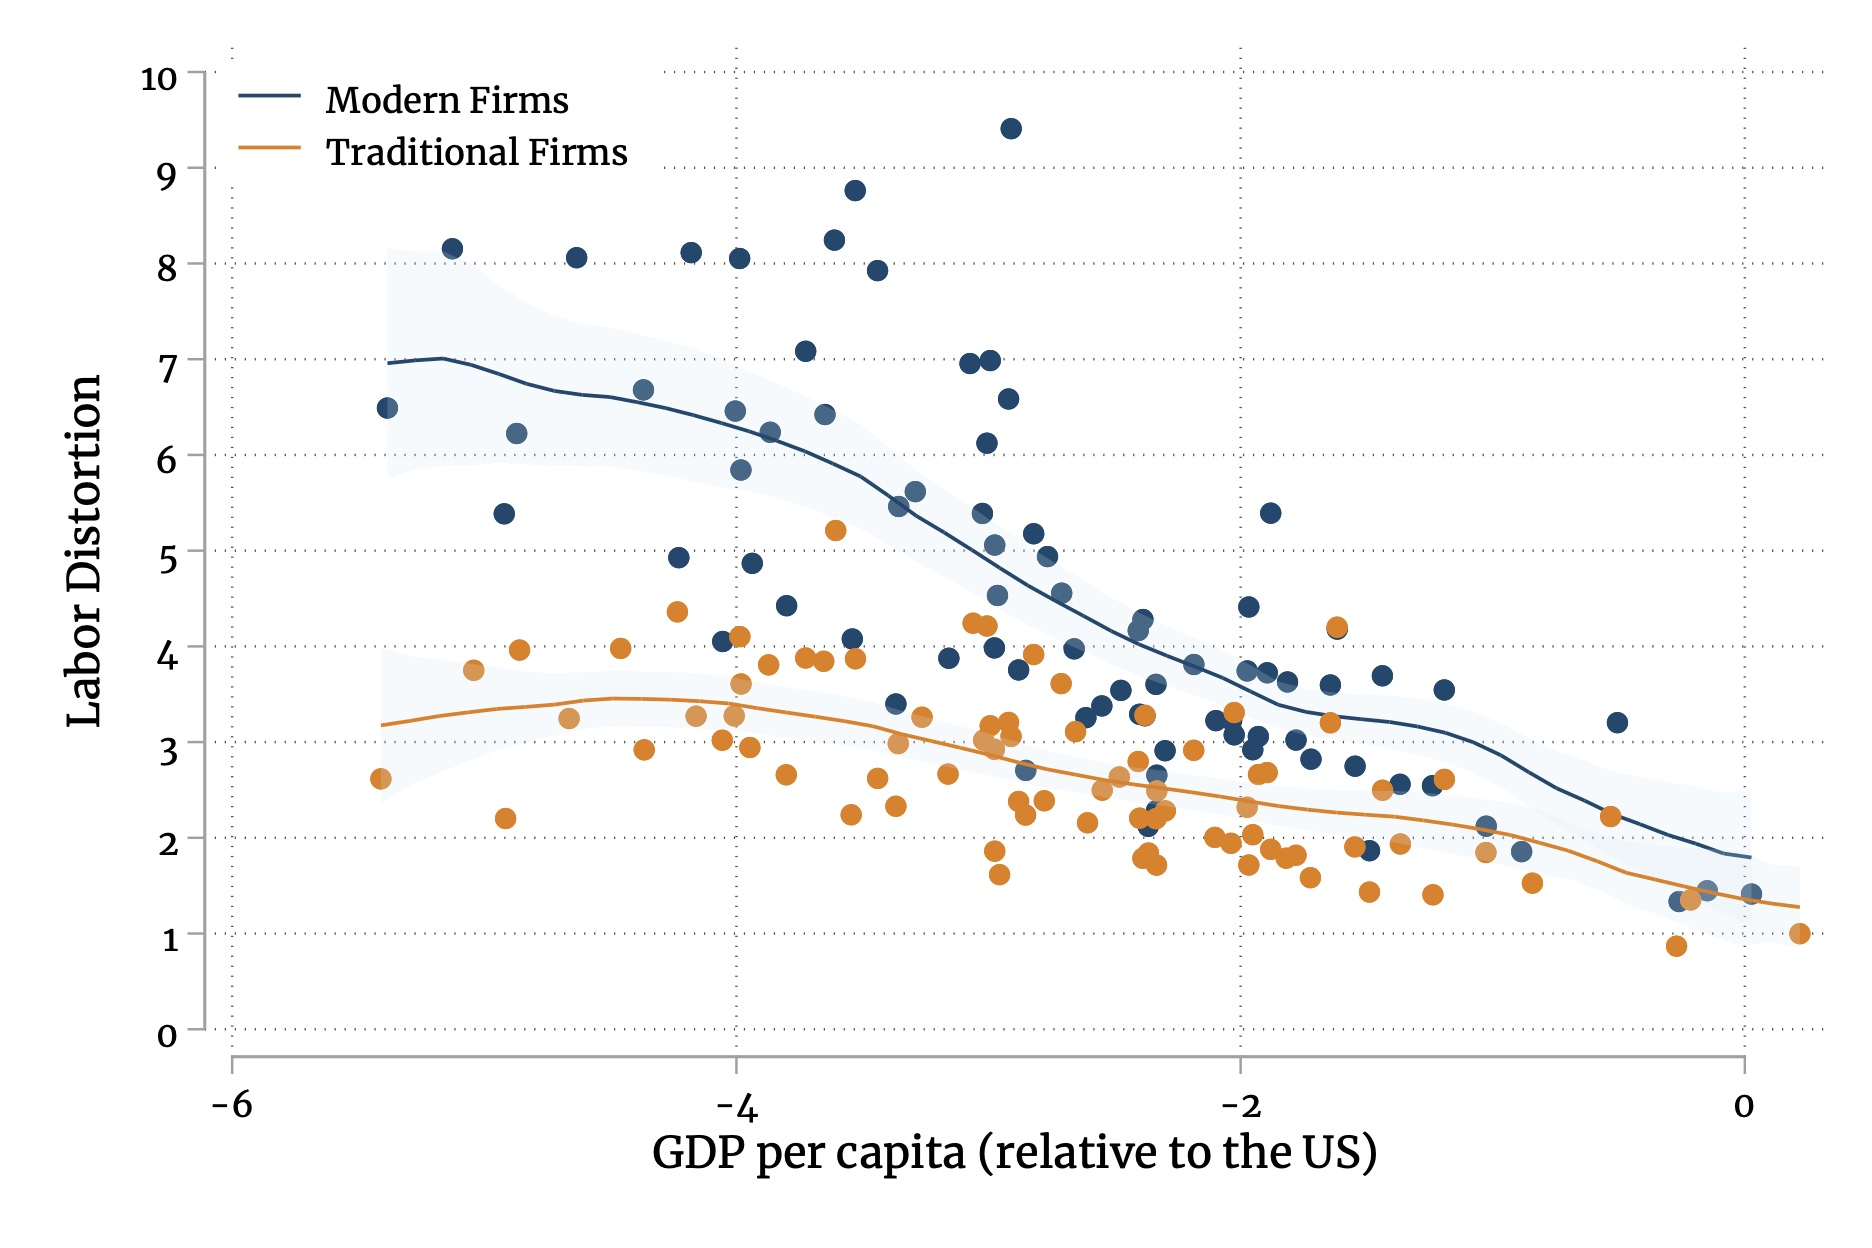
\includegraphics[scale=0.2]{fig/pattern_labor_wedge_cont.jpg}
\par\end{centering}
\textbf{\footnotesize{}Notes}{\footnotesize{}: This figure shows the
distribution of labor wedges across countries at different levels
of economic development. Modern and traditional firms are classified
based on their size. Section \ref{sec:Quantitative-Analyses} describes
the procedure that we use to recover such labor wedges.}{\footnotesize\par}
\end{figure}


\paragraph{Labor Market Distortions and Firm Size in the WBES.}

To close this section, we provide a first look at the firm-level data
from the WBES and show how it speaks to the above-mentioned empirical
patterns from the literature. Figure \ref{fig:fact_section2} reports
our estimates of the labor wedge for modern and traditional firms
(classified based on their size) across countries in different levels
of development\textemdash later, in Section \ref{sec:Model_to_Data},
we describe our classification and estimation procedure. Labor distortions
are generally higher in less developed countries, and particularly
so for modern firms.

Motivated by these aforementioned patterns, our model introduces the
notion that labor wedges can vary by a country's level of economic
development and by the type of technology\textemdash traditional (labor-intensive)
versus modern (intermediate-input-intensive). These differences, in
turn, affect firms' technology choices, and, consequently, the aggregate
exposure of an economy to labor market distortions will depend on
the equilibrium mix of traditional and modern firms.

\section{The Model\label{sec:Model}}

\paragraph*{Environment.}

The global economy consists of multiple countries indexed by $i,\:j\in\mathbb{I}$
and multiple industries indexed by $s,k\in\mathbb{\mathbb{S}}$. Production
in country $i-$industry $s$ can take place under two types of technology
indexed by $t\in\mathbb{T\equiv}\{0,1\}$; namely, ``traditional''
($t=0$) and ``modern'' ($t=1$). Country $i$ is endowed with $\bar{L}_{i}$
units of labor and is populated by a fixed, exogenously given continuum
of firms in each industry, indexed by $\omega\in\Omega_{i,s}$. Each
firm is endowed by one unit of managerial capital. Markets are perfectly
competitive.

\paragraph*{Labor Market Wedges.}

Each economy is subject to wedges in the labor market $\tau_{i,st}^{L}$,
which can vary not only across countries and industries, but also
between modern and traditional technologies. These wedges denote the
difference between the amount a firm pays to employ a worker and the
amount the worker receives.

\subsection{Production}

The production function for firm $\omega\in\Omega_{i,s}$ under technology
$t$ is given by:

\[
Q_{i,st}(\omega)=A_{i,st}\Big(Z_{i,st}(\omega)\,\frac{\mathscr{K}_{i,st}(\omega)}{\gamma_{st}^{Z}}\Big)^{\gamma_{st}^{Z}}\Big(\frac{L_{i,st}(\omega)}{\gamma_{st}^{L}}\Big)^{\gamma_{st}^{L}}\Big(\frac{M_{i,kt}(\omega)}{\gamma_{st}^{M}}\Big)^{\gamma_{st}^{M}},
\]
where $A_{i,st}$ is total factor productivity under technology $t$,
$\mathscr{K}_{i,st}\left(\omega\right)$ is managerial capital, $Z_{i,st}(\omega)$
is the idiosyncratic managerial productivity, $L_{i,st}(\omega)$
is labor employment, and $M_{i,st}(\omega)$ is a composite intermediate
input. Specifically, $M_{i,st}(\omega)=\prod_{s'\in\mathbb{S}}M_{i,ss't}(\omega)^{\phi_{i,ss't}},$
where $M_{i,ss't}(\omega)$ is the bundle of intermediate goods that
industry $s$ purchases from industry $s'$ (that itself aggregates
over inputs sourced from various origin countries), and $\phi_{i,ss'}$
denotes the share corresponding to origin industry $s'$ and destination
industry $s$, with $\sum_{s'}\phi_{i,ss'}=1$. Factor shares are
given by $\gamma_{st}^{Z},\text{\ensuremath{\gamma_{st}^{L}},}$and
$\gamma_{st}^{M}$ and satisfy $\gamma_{st}^{Z}+\gamma_{st}^{L}+\gamma_{st}^{M}=1$.
In particular, $\gamma_{st}^{Z}$ controls the share of payments to
the managerial capital, $\mathscr{K}_{i,st}(\omega)$, that corresponds
to the share of firm's profits, akin to \citet{lucas1978size}.\footnote{Our specification is equivalent to one in which a ``firm'' corresponds
to a manager who employs labor and intermediate inputs under a decreasing-returns-to-scale
production technology. Under this terminology, returns to the managerial
capital should be interpreted as the firm's profits.}

\paragraph*{Firms' Choices of Technology.}

Traditional ($t=0$) and modern technologies ($t=1$) differ in their
input intensity parameters, $\boldsymbol{\gamma}_{0}\equiv\{\gamma_{s0}^{Z},\gamma_{s0}^{L},\gamma_{s0}^{M}\}_{s}$
versus $\boldsymbol{\gamma}_{1}\equiv\{\gamma_{s1}^{Z},\gamma_{s1}^{L},\gamma_{s1}^{M}\}_{s}$,
and total factor productivity levels, $A_{i,s0}$ versus $A_{i,s1}$.
Each firm $\omega\in\Omega_{i,s}$ draws a vector of managerial productivity
levels, $[Z_{i,s0}(\omega),Z_{i,s1}(\omega)]$, and chooses a technology
type. Per cost minimization, the marginal cost of production for a
firm $\omega\in\Omega_{i,s}$ using technology $t$ is:

\[
c_{i,st}(\omega)\equiv\frac{1}{A_{i,st}}\left(\frac{r_{i,st}(\omega)}{Z_{i,st}(\omega)}\right)^{\gamma_{st}^{Z}}\Big(\tau_{i,st}^{L}w_{i}\Big)^{\gamma_{st}^{L}}\Big(m_{i,st}\Big)^{\gamma_{st}^{M}}
\]
where $r_{i,st}\left(\omega\right)$ is the return to managerial capital,
$\tau_{i,st}^{L}w_{i}$ the wage rate in country $i$ inclusive of
labor market wedges, and $m_{i,st}$ the price of the intermediate
input bundle. All firms within a country-industry, regardless of their
technology type, supply the same product. Let $p_{i,s}$ denote the
competitive price supplied by country $i-$industry $s$. Perfect
competition ensures that $p_{i,s}=c_{i,st}(\omega)$, which pins down
firm $\omega$'s profits (as the return to its managerial capital)
when using technology $t$:
\[
r_{i,st}(\omega)=Z_{i,st}(\omega)\,\times\left(a_{i,st}p_{i,s}h_{i,st}/\grave{\tau}_{i,st}^{L}\right)
\]
The firm's profits, $r_{i,st}(\omega)$, depends on output price,
$p_{i,s}$, the technology-specific impact from input prices,
\[
h_{i,st}\equiv\Big(\frac{w_{i}}{p_{i,s}}\Big)^{-\gamma_{st}^{L}/\gamma_{st}^{Z}}\Big(\frac{m_{i,st}}{p_{i,s}}\Big)^{-\gamma_{st}^{M}/\gamma_{st}^{Z}},
\]
the effective labor market wedge, $\grave{\tau}_{i,st}^{L}\equiv\left(\tau_{i,st}^{L}\right)^{\gamma_{st}^{L}/\gamma_{st}^{Z}}$,
the impact of technology-specific productivity, $a_{i,st}\equiv\left(A_{i,st}\right)^{1/\gamma_{st}^{Z}}$,
and the firm-level productivity draw, $Z_{i,st}(\omega)$.\footnote{To provide intuition for how these relative input prices matter, consider
the empirically-relevant case in which the traditional technology
is intensive in the use of labor, and the modern technology is intensive
in the use of intermediate inputs. In that case, within each industry
the return to the traditional technology falls when the relative wage
$\left(w_{i}/p_{i,s}\right)$ increases, and the return to the modern
technology rises if the relative intermediate input price $\left(m_{i,st}/p_{i,s}\right)$
decreases.}

Firm $\omega$ faces a discrete choice problem wherein it chooses
technology $t\in\mathbb{T}$ that maximizes its profits, $r_{i,st}\left(\omega\right)$.
Namely,
\[
\max\left\{ Z_{i,st}(\omega)\times\left(a_{i,st}p_{i,s}h_{i,st}/\grave{\tau}_{i,st}^{L}\right),\quad\mbox{for }t\in\mathbb{T}\right\} .
\]
The vector of firm-level productivities, $\mathbf{Z}_{i,st}(\omega)\equiv\left[Z_{i,st}(\omega)\quad\mbox{for }t\in\mathbb{T}\right]$,
is drawn independently by firms from a Fr�chet distribution, $\Pr\left(\mathbf{Z}_{i,st}(\omega)\leq\mathbf{z}_{i,st}\right)=\exp\left(-\bar{\phi}\sum_{t\in\mathbb{T}}z_{i,st}^{-\theta}\right)$,
where $\bar{\phi}\equiv\left[\Gamma\left(1-1/\theta\right)\right]^{-\theta}$
is a normalization which ensures that $\mathbb{E}\left[Z_{i,st}(\omega)\right]=1$,
with $\theta>1$ governing the dispersion in productivity draws. Under
this distributional assumption, the share of firms that select technology
$t$ in country $i-$industry $s$, denoted by $\alpha_{i,st}$, is:
\begin{equation}
\alpha_{i,st}=\left(\frac{a_{i,st}h_{i,st}/\grave{\tau}_{i,st}^{L}}{H_{i,s}}\right)^{\theta},\quad\mbox{with}\quad H_{i,s}\equiv\left[\sum_{t'\in\mathbb{T}}\left(a_{i,st'}h_{i,st'}/\grave{\tau}_{i,st^{'}}^{L}\right)^{\theta}\right]^{1/\theta};\label{eq: alpha_ist}
\end{equation}
where $H_{i,s}$ is the industry-level average profits (relative to
the output price). Intuitively, a greater share of firms select technology
$t$ if it exhibits $(i)$ a higher average productivity, $a_{i,st}$;
$(ii)$ more favorable impact from wages and intermediate input prices,
as summarized by $h_{i,st}$; and, $(iii)$ lower exposure to labor
market distortions, $\grave{\tau}_{i,st}^{L}$. The extent of these
relationships is controlled by parameter $\theta$, which we call
the ``technology elasticity.''

\paragraph*{Industry Aggregates.}

We can now specify aggregate sales in country $i$\textendash industry
$s$ given firms' choices of technology. Let $R_{i,st}\left(\omega\right)\equiv p_{i,s}Q_{i,st}\left(\omega\right)$
be the sales of firm $\omega\in\Omega_{i,st}$ where $\Omega_{i,st}$
is the set of firms in country $i-$industry $s$ that choose technology
$t$; and by aggregation, $R_{i,st}=\mathbb{E}\left[R_{i,st}(\omega)\:|\:\omega\in\Omega_{i,st}\right]\times|\Omega_{i,s}|$.
Recall that the firm's profits is $r_{i,st}\left(\omega\right)=Z_{i,st}(\omega)\times\left(a_{i,st}p_{i,s}h_{i,st}/\grave{\tau}_{i,st}^{L}\right)$.
Since $r_{i,st}(\omega)$ is a fraction $\gamma_{st}^{Z}$ of firm
$\omega$'s sales, i.e., $R_{i,st}\left(\omega\right)=\left(\gamma_{st}^{Z}\right)^{-1}r_{i,st}\left(\omega\right)$,
the value of sales in country $i-$industry $s-$technology $t$,
$R_{i,st}$, equals:
\[
R_{i,st}=\alpha_{i,st}\times|\Omega_{i,s}|\times\mathbb{E}\left[Z_{i,st}\left(\omega\right)\mid\omega\in\Omega_{is,t}\right]\times\left(\gamma_{st}^{Z}\right)^{-1}\left(a_{i,st}p_{i,s}h_{i,st}/\grave{\tau}_{i,st}^{L}\right).
\]
Since the expected value of productivity draws conditional on firms'
selections equals 
\[
\mathbb{E}\left[Z_{i,st}\left(\omega\right)\mid\omega\in\Omega_{is,t}\right]=\alpha_{i,st}^{-\frac{1}{\theta}},
\]
by normalizing $|\Omega_{i,s}|=1$ (without of loss of generality),
we can derive $R_{i,st}$, as:
\begin{align}
R_{i,st} & =\left(\gamma_{st}^{Z}\right)^{-1}\left(a_{i,st}p_{i,s}h_{i,st}/\grave{\tau}_{i,st}^{L}\right)\left(\alpha_{i,st}\right)^{\frac{\theta-1}{\theta}}\label{eq:R_ist}
\end{align}

Using Equation (\ref{eq:R_ist}), the industry-level sales, $R_{i,s}=\sum_{t\in\mathbb{T}}R_{i,st}$,
can be expressed as:
\begin{equation}
R_{i,s}=p_{i,s}\Gamma_{i,s}^{Z}H_{i,s},\quad\quad\mbox{with}\quad\Gamma_{i,s}^{Z}\equiv\left[\sum_{t\in\mathbb{T}}\alpha_{i,st}\left(\gamma_{st}^{Z}\right)^{-1}\right]^{-1};\label{eq:R_is}
\end{equation}
where $\alpha_{i,st}$ and $H_{i,s}$ are given by Equation (\ref{eq: alpha_ist}).

\subsection{Trade and Consumption}

The representative consumer in each country $j$ receives utility
$C_{j}$ according to a two-tier preference system: 
\[
C_{j}=\prod_{s\in\mathbb{S}}\left(C_{j,s}\right)^{\beta_{j,s}},\quad\quad C_{j,s}=\left[\sum_{i\in\mathbb{I}}\left(b_{ij,s}\right)^{1/\sigma_{s}}\left(C_{ij,s}\right)^{\frac{\sigma_{s}-1}{\sigma_{s}}}\right]^{\frac{\sigma_{s}}{\sigma_{s}-1}}
\]
In the upper tier, the final consumption, $C_{j}$, is a Cobb-Douglas
aggregation over industry-level bundles, $\{C_{j,s}\}_{s\in\mathbb{S}}$,
with constant expenditure shares $\beta_{j,s}$. In the lower tier,
$C_{j,s}$ is a CES aggregation over within-industry varieties that
are differentiated by their origin country, $\{C_{ij,s}\}_{i\in\mathbb{I}}$,
where $b_{ij,s}$ is a demand shifter and $\sigma_{s}$ is the elasticity
of substitution between varieties within industry $s$.

Country $i$'s variety of industry $s$ can be delivered to country
$j$ at price $d_{ij,s}p_{i,s}$, where $p_{i,s}$ is the producer
price and $d_{ij,s}$ is the iceberg trade costs.\footnote{As is standard in the literature, we assume that $d_{ii,s}=1$ and
$d_{ij^{\prime},s}d_{j^{\prime}j,s}>d_{ij,s}$.} We assume that final consumption and intermediate input demand are
characterized by the same CES function, as given by $C_{j,s}$. Accordingly,
country $j$'s share of expenditure on goods originating from country
$i$ within industry $s$ is:

\begin{equation}
\pi_{ij,s}=\frac{b_{ij,s}\left(d_{ij,s}p_{i,s}\right)^{1-\sigma_{s}}}{\left(P_{j,s}\right)^{1-\sigma_{s}}},\quad\quad\mbox{with}\quad P_{j,s}=\left[\sum_{i\in\mathbb{I}}b_{ij,s}\left(d_{ij,s}p_{i,s}\right)^{1-\sigma_{s}}\right]^{\frac{1}{1-\sigma_{s}}};\label{eq:pi_ijs}
\end{equation}
where $P_{j,s}$ denotes the CES price index of industry $s$ in location
$j$.

\subsection{General Equilibrium}

\paragraph*{Market Clearing and Equilibrium.}

The labor market in each country $i$ clears by ensuring that:

\begin{equation}
w_{i}L_{i}=\sum_{s\in\mathbb{S}}\sum_{t\in\mathbb{T}}\left(\frac{1}{\tau_{i,st}}\right)\gamma_{st}^{L}R_{i,st}.\label{eq:mcc_L}
\end{equation}
For each dollar that is paid to employ workers, only a fraction $1/\tau_{i,st}$
is the payment to workers, and the remainder, $\left(\tau_{i,st}-1\right)/\tau_{i,st}$,
is the payment associated with labor wedges. Hence, all else equal,
higher labor wedges lower the demand for workers. In turn, labor wedge
payments amount to:
\begin{equation}
T_{i}=\sum_{s\in\mathbb{S}}\sum_{t\in\mathbb{T}}\left(\frac{\tau_{i,st}-1}{\tau_{i,st}}\right)\gamma_{st}^{L}R_{i,st}.\label{eq:Pi_s}
\end{equation}
The labor wedge represents a range of costs that firms incur due to
labor market distortions, e.g., bribery, theft, bureaucratic berries,
labor market regulations, and search frictions. Our model takes $\tau_{i,st}$
as a reduced-form representation of these distortions without taking
a stance on their specific nature.\footnote{To simplify our analysis and focus on the role of technology choices
and distortions, we adopt the more common approach in which wedges
are exogenous. We leave an analysis of endogenous wedges to future
research.}

The goods market for each country $i-$industry $s$ clears by ensuring
that:
\begin{equation}
R_{i,s}=\sum_{j\in\mathbb{I}}\pi_{ij,s}E_{j,s},\label{eq:mcc_Y}
\end{equation}
where country $i$'s gross expenditure on industry $s$, $E_{i,s}$,
is the sum of final good and intermediate input expenditure:
\begin{equation}
\text{\ensuremath{E_{i,s}}=\ensuremath{\beta_{i,s}Y_{i}}+\ensuremath{\sum_{s'\in\mathbb{S}}\sum_{t\in\mathbb{T}}\left[\phi_{i,s'st}\gamma_{s't}^{M}R_{i,s^{\prime}t}\right]}}.\label{eq:mcc_X}
\end{equation}
Lastly, $Y_{i}$ denotes national income or GDP, and is given by
\begin{equation}
\begin{array}{cl}
Y_{i} & =w_{i}L_{i}+T_{i}+\Pi_{i}\\
 & =\sum_{s\in\mathbb{S}}\sum_{t\in\mathbb{T}}\left(1-\gamma_{i,st}^{M}\right)R_{i,st}
\end{array}\label{eq:mcc_GDP}
\end{equation}
where $\Pi_{i}\equiv\sum_{s\in\mathbb{S}}\sum_{t\in\mathbb{T}}\gamma_{st}^{Z}R_{i,st}$
is the aggregate profits. The above equations ensure that trade is
balanced and the national expenditure net of labor-wedge payments,
$E_{i}-T_{i}$, equals the sum of factor rewards (labor wages and
firms' profits).

In what follows, we refer to $w_{i}L_{i}/P_{i}$ as workers' real
wages and we call real national income,
\begin{equation}
W_{i}\equiv\frac{Y_{i}}{P_{i}}\label{eq:W_i (Welfare)}
\end{equation}
as country $i$'s \emph{welfare,} which in turn corresponds to aggregate
real consumption.

\subsection{Aggregate Labor Productivity (ALP)\label{subsec:Aggregate-Labor-Productivity}}

We define aggregate labor productivity (ALP) in a country-industry
pair as output per worker there\textemdash later we show quantitative
results for alternative measures of ALP. Appendix \ref{subsec:Aggregate-Labor-Productivity (Appendix)}
shows that:

\begin{equation}
\text{ALP}{}_{i,s}\equiv\frac{Q_{i,s}}{L_{i,s}}=\sum_{t}\left[\frac{L_{i,st}}{L_{i,s}}\times\left(\frac{\tau_{i,st}^{L}}{\gamma_{st}^{L}}\frac{w_{i}}{p_{i,s}}\right)\right].\label{eq:ALP_is}
\end{equation}
To see the intuition behind Equation (\ref{eq:ALP_is}), consider
the case of one-sector efficient economy in which labor is the only
factor of production.\footnote{This special case corresponds to: $L_{i,st}\equiv L_{i,t}$, $L_{i,s}\equiv L_{i},$
$p_{i,s}\equiv p_{i}$, $\tau_{i,st}\equiv\tau_{i,t}=1$, and $\gamma_{st}^{L}\equiv\gamma_{t}^{L}=1.$} In that special case, the aggregate labor productivity collapses
to the ratio of wage to producer-price ($w_{i}/p_{i}$). In the general
case, however, labor market distortions and non-labor factors enter
the equation through $\tau_{i,st}^{L}$ and $\gamma_{st}^{L}$. In
addition, one needs to take a stance on how to aggregate industry-level
quantities to a national index of labor productivity. Under the assumption
that industry-level output quantities are aggregated using the final
consumption aggregator, i.e., $Q_{i}=\prod_{s}\left(Q_{i,s}\right)^{\beta_{i,s}}$,
the national-level ALP equals:
\begin{align}
\text{ALP}{}_{i} & \equiv\frac{Q_{i}}{L_{i}}=\left(\frac{w_{i}}{P_{i}}\right)\times\prod_{s}\left[\left(\pi_{ii,s}\right)^{\frac{\beta_{i,s}}{\sigma_{s}-1}}\right]\times\prod_{s}\left[\left(\sum_{t}\ell_{i,st}\times\frac{\tau_{i,st}^{L}}{\gamma_{i,st}^{L}}\right)^{\beta_{i,s}}\right],\label{eq:ALP_i}
\end{align}
where $\ell_{i,st}\equiv L_{i,st}/L_{i}$ is the share of workers
in industry $s-$technology $t$. In words, aggregate labor productivity,
$\text{ALP}{}_{i}$, equals real wage ($w_{i}/P_{i}$) adjusted for:
\emph{(i)} trade openness captured by non-unity domestic expenditure
shares (second bracket), and \emph{(ii)} allocation of workers across
industries and technology types (third bracket). Intuitively, trade
openness alters the relationship between the aggregate produce price
($\prod_{s}p_{i,s}^{\beta_{i,s}}$) and the final consumer price ($P_{i}=\prod_{s}P_{i,s}^{\beta_{i,s}}$);
and, the labor allocation governs the contribution from each industry-technology
pair to the aggregate labor productivity.\medskip{}
\medskip{}

\emph{$ALP$ vs. Welfare.} Our objective is to explore the effects
of trade on aggregate labor productivity $\text{ALP}_{i}$ given by
Equation (\ref{eq:ALP_i}) and welfare $W_{i}$ by Equation (\ref{eq:W_i (Welfare)}).
Linking these two measures of economic performance can, thus, provide
better insight into subsequent results. As shown in Appendix \ref{subsec:Aggregate-Labor-Productivity (Appendix)},
$\text{ALP}_{i}$ relates to welfare per worker $\left(W_{i}/L_{i}\right)$
according to:
\begin{equation}
\underbrace{\text{ALP}_{i}}_{\text{Output per worker}}=\underbrace{\prod_{s}\left[\left(\pi_{ii,s}\right)^{\frac{\beta_{i,s}}{\sigma_{s}-1}}\right]}_{\text{Inverse Terms-of-Trade}}\times\underbrace{\prod_{s}\left[\left(\frac{y_{i,s}}{1-\bar{\gamma}_{i,s}^{M}}\right)^{\beta_{i,s}}\right]}_{\text{Inverse value added share}}\times\underbrace{\left(\frac{W_{i}}{L_{i}}\right)}_{\text{Welfare per worker}},\label{eq: ALP_i vs W_i}
\end{equation}
where $y_{i,s}\equiv Y_{i,s}/Y_{i}$ is the value added share of industry
$s$ in country $i$ and $\bar{\gamma}_{i,s}^{M}$ is the average
cost share of intermediate inputs. Two channels of effect are responsible
for the difference between aggregate labor productivity and welfare.
To see them most clearly, consider a single-industry version of our
setup with one technology type, where the above formula simplifies
to:
\[
\text{APL}_{i}=\pi_{ii}^{\frac{1}{\sigma-1}}\times\frac{1}{1-\bar{\gamma}_{i}^{M}}\times\frac{W_{i}}{L_{i}}.
\]
In a closed economy without intermediate input use, aggregate labor
productivity, $\text{ALP}_{i}$, aligns with welfare per worker, $W_{i}/L_{i}$.
Otherwise, these metrics may diverge based on the terms of trade (represented
by $\pi_{ii}^{\frac{1}{1-\sigma}}$)\footnote{Note that $\pi_{ii}^{\frac{1}{1-\sigma}}=p_{i}/P_{i}$ captures the
terms of trade as the ratio of export price, governed by producer
price $p_{i}$, to import price index, $P_{i}$.} and the share of value added in gross output ($1-\bar{\gamma}_{i}^{M}$).
From this equation, it is evident that welfare and aggregate labor
productivity may react differently to an external event like trade
liberalization in our model, depending on the underlying changes to
the terms of trade and the aggregate value added share.

\subsection{Counterfactual Analysis}

Our framework is adept to study the welfare impacts of changes in
trade costs and labor market wedges.\footnote{In this section, we adopt the hat notation: For any generic variable
$x$ in the baseline equilibrium, let $x^{\prime}$ be its corresponding
value in the counterfactual equilibrium, and $\hat{x}\equiv x^{\prime}/x$
denote its change from the baseline to the counterfactual equilibrium.} Specifically, the sufficient statistics for counterfactual analyses
in our model can be summarized by $\mathscr{B}\equiv\{\mathscr{B}^{\text{Param}},\mathscr{B}^{\text{Data}}\}$
where $\mathscr{B}^{\text{Param}}\equiv\{\sigma,\theta,\gamma_{st}^{L},\gamma_{st}^{M},\gamma_{st}^{Z},\tau_{i,st}^{L},\phi_{i,sk},\beta_{i,s}\}$
and $\mathscr{B}^{\text{Data}}\equiv\{\pi_{ij,s},\alpha_{i,st},w_{i}L_{i},R_{i,st},E_{i,s},Y_{i}\}$.
Given $\mathscr{B}$, for any set of exogenous shocks to trade costs
and labor wedges $\mathscr{P}\equiv\{\hat{d}_{ij,s},\hat{\tau}_{i,st}^{L}\}$,
Appendix \ref{subsec:QGE (Appendix)} describes our model equilibrium
in changes to trade, employment and technology shares, aggregate sales
and expenditures, and prices and wages, $\mathscr{E}\equiv\{\hat{\pi}_{ij,s},$
$\hat{\ell}_{i,st},$ $\hat{\alpha}_{i,st},$ $\hat{R}_{i,st}$ $,\hat{E}_{i,s}$
$,\hat{Y}_{i}$ $,\hat{P}_{i,s}$ $,\hat{p}_{i,s}$ $,\hat{w}_{i}\}$.
Moreover, Appendix \ref{sec:Welfare-and-Productivity-Derivations (appendix)}
derives the change to welfare, real wage, and aggregate labor productivity
as a function of the above sufficient statistics and general equilibrium
changes to domestic expenditure shares ($\hat{\pi}_{ii,s}$), employment
shares ($\hat{\ell}_{i,st}$), and technology shares ($\hat{\alpha}_{i,st}$).

\section{Misallocation\emph{ }and the Gains from Trade\label{sec:Misallocation-and-Gain-from-trade}}

This section explores the impacts of labor market distortions on the
gains from trade, emphasizing the role of technology adoption. To
set the stage for an open-economy analysis, we first characterize
the cost of misallocation in closed economy. We then return to our
general open economy setup to characterize the effects of trade liberalization
on two aggregate outcomes: welfare and aggregate labor productivity.
We draw connections to the canonical ACR framework, discussing the
role of labor market distortions and technology adoption.

\paragraph*{Employment and Output Shares.}

In what follows, we define additional share variables. We use $\rho_{i,st}$
to denote the share of technology $t$ from total output (sales) of
country $i$\textendash industry $s$; $r_{i,s}$ to denote the share
of industry $s$ from output in country $i$; and $\ell_{i,st}$ to
denote the share of labor employed by industry $s$\textendash technology
$t$ in country $i$.\footnote{See Appendix \ref{subsec: Shares (Appendix)} for how $\rho_{i,st}$
and $\ell_{i,st}$ can be inferred from firm-technology shares, $\alpha_{i,st}$.} Stated formally,
\begin{equation}
\rho_{i,st}\equiv\frac{R_{i,st}}{\sum_{t'}R_{i,st'}};\quad\quad r_{i,s}=\frac{\sum_{t}R_{i,st}}{\sum_{s'}\sum_{t}R_{i,s't}};\quad\quad\ell_{i,st}\equiv\frac{L_{i,st}}{L_{i}}\label{eq:Shares_Definition}
\end{equation}


\subsection{Misallocation and Inefficient Technology Adoption\label{subsec:Cost-of-Missallocation}}

In our model, labor market wedges ($\tau_{i,st}^{L}$) create two
sources of misallocation. First, given technology choices, employment
shares are inefficiently low in firms using high-$\tau^{L}$ technologies.
Second, labor market wedges lead to inefficiently low adoption of
high-$\tau^{L}$ technologies. Since empirically modern technologies
are subject to higher labor market wedges (Section \ref{fig:fact_section2}),
misallocation will manifest as inefficiently low adoption of modern
technologies as well as low labor employment by modern firms.

To communicate this point transparently, this section provides an
exact formula for the cost of misallocation in a closed economy, which
isolates the cost of misallocation from terms of trade effects. In
addition, we assume that firms employ only primary factors of production
(i.e., no intermediate inputs) ($\gamma_{st}^{M}=0$), that factor
intensities are symmetric across technologies ($\boldsymbol{\gamma}_{0}=\boldsymbol{\gamma}_{1}$),
and that the economy has a single-sector\textemdash similar formulas
apply to the multi-sector case (Appendix \ref{sec: Misallocation Formula (Appendix)}).
In this section, we therefore drop the index for sectors.

We define the welfare cost of misallocation, $\mathcal{D}_{i}$, as
the (log) welfare distance to the Pareto-efficient frontier. We, moreover,
define
\[
\widetilde{\tau}_{i,t}^{L}\equiv\tau_{i,t}^{L}/\mathbb{E}_{\ell}\left[\tau_{i,t}^{L}\right]
\]
as the normalized wedge associated with technology $t$, with $\mathbb{E}_{\ell}\left[\tau_{i,t}^{L}\right]\equiv\sum_{t}\left[\ell_{i,t}\tau_{i,t}^{L}\right]$
denoting the employment-weighted average wedge in country $i$. As
shown in Appendix \ref{sec: Misallocation Formula (Appendix)}, the
welfare cost of misallocation is
\begin{equation}
\mathcal{D}_{i}=\frac{\bar{\gamma}_{i}^{Z}}{\theta}\log\mathbb{E}_{\ell}\left[\left(\tilde{\tau}_{i,t}^{L}\right)^{1+\frac{\bar{\gamma}_{i}^{L}}{\bar{\gamma}_{i}^{Z}}\theta}\right]\label{eq:misallocation_cost_noapp}
\end{equation}
where $\bar{\gamma}_{i}^{L}$and $\bar{\gamma}_{i}^{Z}$ denote aggregate
labor and managerial capital intensity in economy $i$, and $\mathbb{E}_{\ell}\left[.\right]$
denotes the employment-weighted mean.

Equation (\ref{eq:misallocation_cost_noapp}) reveals that misallocation
occurs only if labor market wedges exhibit dispersion from the mean.
In particular, a common wedge $\tau_{i,t}^{L}=\tau_{i}^{L}$ that
applies equally to all technologies will amount to $\tilde{\tau}_{i,t}^{L}=1$
and zero misallocation. To further underscore the role of technology
adoption, we can examine the second-order approximation of $\mathcal{D}_{i}$
for small departures from a common wedge: 
\begin{equation}
\mathcal{D}_{i}\approx\ \frac{\bar{\gamma}_{i}^{L}}{2}\left(1+\frac{\bar{\gamma}_{i}^{L}}{\bar{\gamma}_{i}^{Z}}\theta\right)\text{\ensuremath{\text{Var}_{\ell}\left[\widetilde{\tau}_{i,t}^{L}\right]}},\label{eq:misallocation_cost_app}
\end{equation}
where $\text{Var}_{\ell}\left[\widetilde{\tau}_{i,t}^{L}\right]$
is the variance of normalized labor wedges or the coefficient of variation
of actual wedges. There are two takeaways from the above approximation.
First, it reveals that dispersion from the mean (rather than the mean
level of wedges) determines the welfare cost of misallocation\textemdash This
observation is crucial, considering our earlier finding that labor
wedges exhibit greater dispersion across traditional and modern technologies
in low-income countries. Second, it highlights the misallocation-magnifying
effects of technology adoption. Misallocation without endogenous technology
adoption would simply amount to $\frac{\bar{\gamma}_{i}^{L}}{2}\text{Var}_{\ell}\left[\widetilde{\tau}_{i,t}^{L}\right]$.
However, when firms' endogenous technology choices are distorted by
labor wedges, misallocation is amplified by an additional amount $\frac{\bar{\gamma}_{i}^{L}}{2}\times\frac{\bar{\gamma}_{i}^{L}}{\bar{\gamma}_{i}^{Z}}\theta\text{Var}_{\ell}\left[\widetilde{\tau}_{i,t}^{L}\right]$.
In other words, misallocation occurs because, first, there is insufficient
adoption of modern, high-$\tau^{L}$ technologies and, second, there
is insufficient labor employment by firms that adopt modern, high-$\tau^{L}$
technologies.

\subsection{Impact of Trade on Welfare\label{subsec:Impact-of-Trade-on-Welfare-Theory}}

This section presents two sets of formulas for the \emph{welfare}
effects of trade in our framework, regarding: \emph{(i)} welfare decomposition
in response to a piecemeal trade liberalization and\emph{ (ii)} welfare
gains of moving economies from autarky to their observed equilibrium.
Appendix \ref{sec:Welfare-and-Productivity-Derivations (appendix)}
presents derivations for this section.

\subsubsection{Decomposing the Ex-Ante Welfare Gains from Piecemeal Trade Liberalization\label{subsec:Decomposing-Welfare-Using-Ex-Ante-Gains-Thoery}}

In our framework, trade liberalization influences technology choices
and the allocation of primary inputs across firm types, which in turn
affects the degree of misallocation. Here, we elucidate, analytically,
how these mechanisms shape welfare, connecting our results to the
canonical ACR formula.

We start by presenting a decomposition of trade-driven welfare effects.
For a crisp decomposition, we consider a small shock to trade costs,
$\left\{ \text{d}\ln d_{ij,s}\right\} _{i,j,s}$, which delivers the
following change in log welfare:\vspace{-0.1in}
\begin{align}
\text{d}\ln W_{i}= & \overbrace{\sum_{s,k}\left[\beta_{i,s}\varphi_{i,sk}\frac{1}{1-\sigma_{k}}\text{d}\ln\pi_{ii,k}\right]}^{\text{ACR}}+\overbrace{\left(\frac{\bar{\gamma}_{i}^{L}}{1-\bar{\gamma}_{i}^{M}}\right)\text{Co\ensuremath{v_{\ell}}}\left[\widetilde{\tau}_{i,st}^{L},\text{d}\ln\ell_{i,st}\right]}^{\Delta\left(\text{Allocative Efficiency}\right)}\label{eq:dlnW_i_Piecemeal}\\
 & +\ \underbrace{\sum_{k,t}\left[\gamma_{kt}^{Z}\rho_{i,kt}\left(\Lambda_{i,k}-\sum_{s}\beta_{i,s}\varphi_{i,sk}\right)\text{d}\ln\ell_{i,kt}\right]}_{\text{Residual ToT via Int'l Profit Transfers}}\nonumber \\
 & +\ \underbrace{\sum_{k,t}\left[\gamma_{kt}^{Z}\rho_{i,kt}\left(\sum_{s}\beta_{i,s}\varphi_{i,sk}\right)\left(\frac{\theta-1}{\theta}\right)\text{d}\ln\left(\alpha_{i,kt}\right)\right]}_{\text{Residual Technology Selection Effect}}\nonumber 
\end{align}
In the above equation, $\varphi_{i,sk}$ corresponds to entry $\left(s,k\right)$
of country $i$'s Leontief inverse matrix and $\Lambda_{i,s}\equiv p_{i,s}Q_{i,s}/Y_{i}$
denotes the \emph{Domar} weight of industry $s$ in country $i$.

The first term (on the right-hand side) corresponds to the ACR formula
for the gains from final good and intermediate input trade.

The second term represents the change in allocative efficiency and
is positive if trade liberalization directs workers toward modern
(high\textendash $\tau$) technologies and industries\textemdash i.e.,
if $\text{Co\ensuremath{v_{\ell}}}\left[\widetilde{\tau}_{i,st}^{L},\text{d}\ln\ell_{i,st}\right]>0$.
This term becomes zero when the economy is efficient (i.e., when $\widetilde{\tau}_{i,st}^{L}=1$
for all $s$ and $t$). Otherwise, trade liberalization can increase
allocative efficiency by reallocating workers toward modern firms,
echoing our previous assertion that (absent trade) modern technologies
exhibit inefficiently low employment shares. Moreover, trade liberalization
also reallocates workers toward industries where a country has a comparative
advantage. If the comparative-advantage industries are less-exposed
to labor market distortions, trade may reduce allocative efficiency
through inter-industry reallocation.\footnote{In our quantitative analyses, we mainly focus on the impact of trade
openness through technology choices. For that reason and also due
to data limitations, our estimation assumes that labor market distortions
vary only between technology types and are common for a technology
type across industries.}

The third and fourth terms encompass residual terms of trade effects
via international profit transfers (not accounted by the ACR term)
and residual technology selection effects (not accounted by the ACR
or Allocative Efficiency terms). The residual terms of trade (ToT)
effects reflect the change in firms' profits, a fraction of which
is paid for by foreign consumers. To see this, note that if country
$i$ was operating as a closed economy, market-clearing identities
would imply $\Lambda_{i,k}-\sum_{s}\beta_{i,s}\varphi_{i,sk}=0$;
indicating that any possible welfare gains from higher profits are
neutralized by a proportional increase in the domestic price index.
In the open economy case, by contrast, $\Lambda_{i,k}-\sum_{s}\beta_{i,k}\varphi_{i,sk}\neq0$,
reflecting decoupling between domestic production and consumption.
As such, a change to firms' profits can lead to improvements in the
terms of trade, depending on what fraction of the profits are paid
for by foreign versus domestic consumers. The term $\left[\gamma_{kt}^{Z}\rho_{i,kt}\times\left(\Lambda_{i,k}-\sum_{s}\beta_{i,s}\varphi_{i,sk}\right)\text{d}\ln\ell_{i,kt}\right]$
represents these terms-of-trade effects.\footnote{\label{fn:welfare-one-sector}Generally, the Residual ToT Effects
emerge due to the potential discrepancy between the vectors of consumption
shares and production shares. In addition to the case of closed economy,
this discrepancy disappears in the case of a one-sector economy, where
the welfare decomposition formula collapses to:
\begin{align*}
\text{d}\ln W_{i}= & \overbrace{\left(\frac{1}{1-\bar{\gamma}^{M}}\right)\left[\frac{1}{1-\sigma}\text{d}\ln\pi_{ii}\right]}^{\text{ACR}}+\overbrace{\left(\frac{\bar{\gamma}_{i}^{L}}{1-\bar{\gamma}_{i}^{M}}\right)\text{Cov}_{\ell}\left[\widetilde{\tau}_{i,t}^{L},\text{d}\ln\ell_{i,t}\right]}^{\Delta\left(\text{Allocative Efficiency}\right)}\\
 & +\underbrace{\left(\frac{1}{1-\bar{\gamma}^{M}}\right)\left[\sum_{t}\rho_{i,t}\gamma_{t}^{Z}\left(\frac{\theta-1}{\theta}\right)d\ln\left(\alpha_{i,t}\right)\right]}_{\text{Residual Technology Selection Effects}}.
\end{align*}
} The residual technology selection effects capture how the selection
of firms into the different technology types, reflected by $\text{d}\ln\left(\alpha_{i,kt}\right)$,
influences aggregate managerial productivity. When the output of a
technology type increases, infra-marginal managers that select that
technology are less productive than those who already selected it.
In one extreme with $\theta\rightarrow\infty$, this margin of adjustment
comes with no dampening effect on aggregate profits corresponding
to the case where managerial capital in each industry is perfectly
mobile between technology types. In the other extreme with $\theta\rightarrow1$,
the entire term collapses to zero, corresponding to the case where
the production technology at the aggregate level of industries uses
managerial capital as a specific factor.

\subsubsection{Ex-Post Welfare Gains from Trade\label{subsec:Ex-Post-Gains-from-Trade-Theory}}

We produce sufficient statistics formula for the ex post gains from
trade, defined as the change to welfare from moving a country from
a counterfactual autarky state to its baseline (observed) equilibrium.
For clarity, we present our formula for a single-industry version
of our model. Appendix \ref{subsec:Ex-post-Gains_apdx} shows that
the gains from trade in this case can be expressed as:
\[
\text{GT}_{i}=1-\Delta_{i}\times\pi_{ii}^{\frac{1}{\sigma-1}},
\]
where $\pi_{ii}$ denotes the domestic expenditure share, and the
country-specific multiplier, $\Delta_{i}$, solves the following equation:
\[
\sum_{t}\left[\alpha_{i,t}\left(\hat{\Gamma}_{i,t}\left(\pi_{ii}^{\frac{1}{\sigma-1}}\right)^{\frac{\gamma_{t}^{M}}{\gamma_{t}^{Z}}}\left(\Delta_{i}^{-1}\right)^{\frac{1-\gamma_{t}^{M}}{\gamma_{t}^{Z}}}\right)^{\theta}\right]^{\frac{1}{\theta}}=1.
\]
In this formula, $\hat{\Gamma}_{i,t}$ encapsulates the welfare-relevant
change to factor intensities, which can be solved as a function of
the multiplier $\Delta_{i}$, baseline technology shares, $\alpha_{i,t}$,
technology-specific factor intensity parameters and labor wedges,
as detailed in Appendix \ref{subsec:Ex-post-Gains_apdx}. In a special
case where production uses only one type of technology ($\alpha_{0}=1$,
$\alpha_{1}=0$, and $\gamma_{1}^{M}\equiv\gamma^{M}$), $\hat{\Gamma}_{i,t}$
collapses to unity and $\Delta_{i}=\pi_{ii}^{\frac{1}{\sigma-1}\frac{\gamma^{M}}{1-\gamma^{M}}}$.
In that case, our gains-from-trade formula reduces to the standard
ACR formula under the roundabout technology: 
\[
\text{GT}_{i}^{\text{ACR}}=1-\pi_{ii}^{\frac{1}{1-\gamma^{M}}\frac{1}{\sigma-1}}.
\]

Generally, beyond this special case, $\Delta_{i}$ adjusts the gains
from trade particularly to account for trade-led changes to allocative
efficiency. Specifically, compared to ACR, here a new mechanism is
at play: By improving firms' access to foreign intermediate goods,
trade encourages firms to shift toward modern, intermediate-input-intensive
technologies. This trade-induced modernization of industries improves
aggregate productivity. Moreover, modern firms are subject to higher
labor market distortions, therefore this modernization process can
improve the allocative efficiency. Section \ref{subsec:Ex-Post-Gains-Welfare-Quantitative}
compares the welfare gains-from-trade in our model, $\text{GT}_{i}=1-\Delta_{i}\times\pi_{ii}^{\frac{1}{\sigma-1}}$
with the special case of $\text{GT}_{i}^{\text{ACR}}=1-\pi_{ii}^{\frac{1}{1-\gamma}\frac{1}{\sigma-1}}$.

\subsection{Impact of Trade on Aggregate Labor Productivity\label{subsec:Impact-of-Trade-on-ALP-Theory}}

We now examine the effects of a small shock to trade costs on aggregate
labor productivity (ALP), expressed in Equation (\ref{eq:ALP_i}).
Here, for a clearer exposition, we present the formula for a single-sector
version of the model:

\begin{align}
\text{d}\ln\left(\text{ALP}_{i}\right) & =\ \left(\frac{\bar{\gamma}_{i}^{M}}{1-\bar{\gamma}_{i}^{M}}\right)\,\frac{1}{1-\sigma}\text{d}\ln\pi_{ii}\label{eq:dlnALP_i}\\
 & \ \ +\left(\frac{1}{1-\bar{\gamma}_{i}^{M}}\right)\left[\text{Cov}_{\ell}\left(\left[1-\bar{\gamma}_{i}^{M}-\gamma_{t}^{Z}\right]\tilde{\delta}_{i,t},\text{d}\ln\ell_{i,t}\right)+\left(\frac{\theta-1}{\theta}\right)\sum_{t}\gamma_{t}^{Z}\rho_{i,t}\text{d}\ln\alpha_{i,t}\right]\nonumber 
\end{align}
where $\bar{\gamma}_{i}^{M}$ is average cost share of intermediate
input use, $\rho_{i,t}$ is the output share defined by Equation (\ref{eq:Shares_Definition}),
and $\tilde{\delta}_{i,t}$ denotes the deviation of labor-wedge-to-labor-intensity
ratio from its mean: 
\[
\tilde{\delta}_{i,t}^{L}\equiv\frac{\delta_{i,t}^{L}}{\mathbb{E}_{\ell}\left[\delta_{i,t}^{L}\right]}=\frac{\delta_{i,t}^{L}}{\sum_{t'}\left(\delta_{i,t'}^{L}\ell_{i,t'}\right)},\qquad\text{where}\qquad\delta_{i,t}^{L}\equiv\frac{\tau_{i,t}^{L}}{\gamma_{i,t}^{L}}.
\]
The above formula decomposes the impacts of trade liberalization on
aggregate labor productivity into three effects: First, trade liberalization
provides improved access to foreign intermediate inputs that complement
primary inputs, thereby raising labor (and managerial capital) productivity.
These productivity gains are represented by the first term on the
right-hand side of Equation (\ref{eq:dlnALP_i}).\footnote{To see the connection more clearly, note that an increase in trade
openness ($\text{d}\ln\pi_{ii}<0$) raises ALP via the the first term
on the right-hand side, and more so the higher the average input intensity,
$\bar{\gamma}_{i}^{M}$.} Second, trade liberalization reallocates workers from one type of
technology to another where primary inputs exhibit different marginal
productivity levels. These \emph{allocative effects} are encapsulated
by the second term on the right-hand side. Third, trade liberalization
prompts \emph{technology choices}. These selection effects are partly
encapsulated by the second term (as they regulate $\text{d}\ln\ell_{it}$)
and partly by the last term on the right-hand side of Equation (\ref{eq:dlnALP_i}).
The latter two effects (allocative effects and technology choices)
distinguish our framework from standard models.\footnote{These three components are comparable to the ones in our welfare decomposition
(compare with the one-sector formula in footnote \ref{fn:welfare-one-sector}).
However, the effect on ALP along each of these three channels is different
from their effect on welfare, because the gross output of each country
is different from its aggregate real consumption.}

\section{Bringing the Model to Data\label{sec:Model_to_Data}}

To run counterfactual analyses, we simulate our model in changes based
on the exact hat algebra approach as in \citet{dekle2007unbalanced},\footnote{Appendix \ref{subsec:QGE (Appendix)} describes our model equilibrium
in changes, and the numerical algorithm that we employ to simulate
it.} which allows us to sidestep the parametrization of TFPs and trade
costs. Table \ref{tab:Sufficient-Statistics} summarizes the required
parameters and the summary statistics to simulate our model. Below,
we briefly explain our calibration, relegating details to Appendix
\ref{sec:Quantification_apdx}.

We combine country-level aggregates from the GTAP data with firm-level
statistics and estimates obtained from the WBES data. From the GTAP
database, we take global flows from each origin country-industry to
each destination country-industry, as well as value added shares,
for the year 2014. A key feature of GTAP, relative to other Input-Output
datasets, is that it covers a wide range of countries in different
levels of economic development. From the WBES, we obtain our estimates
of technology-specific labor wedges and elasticities of output with
respect to labor, and the share of modern firms in each country.\footnote{By and large, our focus is on manufacturing. The WBES data, also,
inform us only about manufacturing industries. Consequently, we collapse
each of our non-manufacturing industries (agriculture, mining, and
services) into only one technology type. To set labor wedges in non-manufacturing,
we use their averages across the two manufacturing technologies. We
take all other information for the non-manufacturing industries from
the GTAP database, with no need for more disaggregated data.} Important for us, WBES also provides firm-level data across countries
in different levels of economic development\textemdash approximately
90,000 firms operating between 2006-2020 across 140 countries. We
first split the sample of firms into two types, modern and traditional,
based on their total sales, using a simple clustering approach akin
to \citet{asturias2019grouped}.\footnote{We consider this classification as a \emph{proxy }for technology adoption,
given that the data provide us with no additional information for
a classification. For a subset of countries, however, we have information
on whether firms are in the formal of in the informal sector. Hence,
in Section \ref{subsec:Robustness}, we experiment with an alternative
classification in which we assign formal firms to the modern technology
and informal firms to the traditional one.} We then estimate output elasticities of labor, for each technology
type, using the control function approach \citep{levinsohn2003estimating,olleypakes1996}.
The remaining input elasticities are calibrated to match aggregate
statistics on the cost share of labor, the cost share of intermediate
inputs, and firm size. Lastly, with estimates of output elasticity
in hand, we recover labor wedges for each country and technology type.

Two empirical patterns emerge from our calibration that are in line
with the motivating evidence from the literature which we discussed
in Section (\ref{sec:motivating_evidence}). First, labor market wedges
are larger for modern firms, and significantly more so in low-income
countries economies. Second, modern firms use labor less intensively
than traditional firms.\footnote{In Appendix Section \ref{subsec:Robustness}, we discuss alternative
approaches and robustness tests for the estimation of production function
and labor wedges. The key patterns that emerge from our preferred
calibration holds across a wide range of alternative approaches. Moreover,
in Section \ref{subsec:Robustness}, we also experiment with alternative
calibrations of the model and show that our overall conclusions remain
the same.}

In addition, we set the trade elasticity, $(\sigma-1)$, to 3 in line
with available estimates in the literature (\citet{simonovska2014elasticity},
\citet{imbs2015elasticity}). We pick the technology elasticity, $\theta$,
from \citet{farrokhipellegrina} who estimate a comparable elasticity
for the agriculture sector\textemdash Section \ref{subsec:apx_alternative_thetas}
experiments with alternative values of $\theta$.

Our final sample consists of 99 countries plus an aggregate for the
rest of the world and 14 industries\textemdash consisting of 11 manufacturing
and 3 non-manufacturing industries.
\begin{table}[th]
\caption{Calibration and Sufficient Statistics\label{tab:Sufficient-Statistics}}

\begin{centering}
{\small{}}%
\begin{tabular}{lll}
\hline 
{\small{}Description} & {\small{}Parameter} & {\small{}Value/Source}\tabularnewline
\hline 
{\small{}Trade elasticity} & {\small{}$\sigma_{s}-1$} & {\small{}3.0 \citep{simonovska2014elasticity}}\tabularnewline
{\small{}Technology elasticity} & {\small{}$\theta$} & {\small{}4.5 \citep{farrokhipellegrina}}\tabularnewline
{\small{}Share of modern firms} & {\small{}$\alpha_{i,kt}$} & {\small{}Clustering, WBES}\tabularnewline
{\small{}Labor wedges} & {\small{}$\tau_{i,t}^{L}$} & {\small{}Estimated, WBES}\tabularnewline
{\small{}Output elasticity of labor} & {\small{}$\gamma_{t}^{L}$} & {\small{}Estimated, WBES}\tabularnewline
{\small{}Output elasticity of other inputs} & {\small{}$\gamma_{t}^{M}$ and $\gamma_{t}^{Z}$} & {\small{}Aggregates from GTAP and WBES}\tabularnewline
{\small{}Consumption shares} & {\small{}$\beta_{i,s}$ and $\phi_{i,ss't}$} & {\small{}Expenditure shares, GTAP}\tabularnewline
{\small{}Trade shares} & {\small{}$\pi_{ij,s}$} & {\small{}GTAP}\tabularnewline
\hline 
\end{tabular}{\small\par}
\par\end{centering}
\textbf{\footnotesize{}Notes}{\footnotesize{}: This table reports
the set of sufficient statistics, and their data sources, that we
employ to calculate counterfactual changes in our general equilibrium
model. We simulate the model based on the exact hat algebra which
allows us to sidestep the need to calibrate total factor productivities
and trade costs. Appendix \ref{sec:Quantification_apdx} details the
calibration procedure.}{\footnotesize\par}
\end{table}


\section{Quantitative Analyses\label{sec:Quantitative-Analyses}}

Having the calibrated model in hand, we now undertake two sets of
quantitative exercises. First, we consider the welfare effects of
trade. Specifically, we examine the aggregate \emph{ex-ante} gains
from piecemeal trade liberalization, using our welfare decomposition
formula from Section \ref{subsec:Decomposing-Welfare-Using-Ex-Ante-Gains-Thoery}
to isolate the role of technology adoption and distortions from standard
ACR effects. We then compute the aggregate \emph{ex-post} gains from
trade, connecting more directly our results to the standard gains
from trade implied by the ACR formula. Second, we examine the impact
of trade on aggregate labor productivity. In the spirit of a difference-in-differences
design, we simulate a set of counterfactuals to determine the impact
of trade liberalization on labor productivity, \emph{with} and \emph{without}
distortions.

Before presenting our main quantitative results for open economies,
let us briefly report the welfare cost of labor market distortions
in the counterfactual where countries operate as closed economies\textemdash mimicking
our discussion in Section \ref{subsec:Cost-of-Missallocation}. We
find that the welfare cost of misallocation is six times larger in
low-income countries relative to their high-income counterparts, reflecting
the fact that the cross-technology dispersion in labor market wedges
is remarkably higher in low-income countries (Appendix Figure \ref{fig:Welfare_Cost_Closed}).
Additionally, higher technology elasticity, $\theta$, magnifies the
welfare cost of misallocation, underscoring the role of technology
adoption as indicated by Equation (\ref{eq:misallocation_cost_app}).

\subsection{Welfare Effects of Trade\label{subsec:Welfare-Effects-Quantitative}}

\subsubsection{Decomposing Ex-Ante Welfare Gains from Trade Liberalization\label{subsec:Ex-Ante-Welfare-Gains-Quantitative}}

In this section, we simulate a piecemeal trade liberalization, one
country at a time, by counterfactually lowering the trade costs associated
with a country's exports and imports. We then use Equation (\ref{eq:dlnW_i_Piecemeal})
to decompose the resulting welfare effects into \emph{ACR,} \emph{Allocative
Efficiency,} \emph{Residual Effects (Residual Terms of Trade via International
Profit Transfers plus Residual Technology Selection Effects).}

Table \ref{tab:GFT-Piecemeal} presents our results, reporting average
outcomes for countries in the low-income, middle-income and high-income
brackets. A key finding is that the contribution of the \emph{non-ACR}
terms is consistently positive, indicating that the welfare gains
from trade liberalization exceed those implied by the standard ACR
formula. Moreover, the non-ACR welfare effects are relatively larger
among low-income countries. Roughly 20\% of the welfare gains from
trade liberalization are attributable to non-ACR effects among low-income
countries, versus less than 10\% in their high-income counterparts.\footnote{The Residual Effects almost entirely are accounted for by \emph{Residual
Terms of Trade via International Profit Transfers}. The contribution
from the \emph{Residual Technology Selection Effect} is virtually
zero in this exercise because on the aggregate the negative effect
of the shrinking technology almost entirely cancels out the positive
effect of the expanding technology.}

Note that trade liberalization improves allocative efficiency at all
income levels. Intuitively, trade liberalization lowers the price
of imported intermediate inputs, thereby directing resources towards
modern technologies and encouraging their adoption. Both mechanisms
reduce misallocation, which, recall, stems from inefficiently low
production by modern firms and insufficient adoption of modern technologies,
generated by larger exposure of modern firms to larger labor distortions
vis-�-vis traditional ones. Notably, improvements to allocative efficiency
constitute a larger portion of the overall gains from trade liberalization
in low-income countries, given their higher initial levels of misallocation
(see Appendix Figure \ref{fig: trade vs APL (appendix)}).
\begin{table}[th]
\caption{Decomposition: Ex Ante Gains from Trade Liberalization\label{tab:GFT-Piecemeal}}

\begin{table}[H] 	
\centering
\footnotesize 	
\begin{tabular}{lccc} \hline
& ACR & Allocative Efficiency & Residual Effects \\ \hline
High income   & 90.3\% & 3.0\% & 6.7\% \\     
Middle income & 86.6\% & 5.0\% & 8.4\% \\     
Low income    & 81.2\% & 9.2\% & 9.6\% \\ \hline
\end{tabular}
\end{table}
\vspace{-0.2in}

\textbf{\footnotesize{}Notes}{\footnotesize{}: This table shows the
contribution of each listed component to the welfare gains from a
local reduction in trade costs of each country. The results show the
average values across countries in the three groups of high-income,
middle-income and low-income countries. The three components of the
welfare change are shown in Equation (\ref{eq:dlnW_i_Piecemeal}),
referred to as ACR, Allocative Efficiency and Residual Effects. The
Residual Effects are almost entirely accounted for by Residual Terms
of Trade via International Profit Transfers, with the contribution
from the Residual Technology Selection Effect to be virtually zero.}{\footnotesize\par}
\end{table}


\subsubsection{Ex-Post Welfare Gains from Trade\label{subsec:Ex-Post-Gains-Welfare-Quantitative}}

We now turn to evaluate the \emph{ex-post} gains from trade in our
framework, comparing them to the gains from trade implied by the canonical
ACR formula. Following the literature, we define the ex-post gains
from trade as the welfare gains of moving from autarky to the observed
equilibrium.

Table \ref{tab:GFT} reports the average gains from trade across low-income,
middle-income, and high-income countries. Our framework implies larger
gains from trade than ACR: 21.3\% versus 19.3\% for high-income countries,
20.0\% versus 18.0\% for middle-income countries, and 19.3\% versus
\% for low-income countries. The greater gains implied by our model
emanate from trade's ability to correct misallocation. Shutting down
trade in our framework directs resources towards traditional technologies
and incentivizes firms to pivot from modern to traditional technologies.
These mechanisms exacerbate misallocation in the economy, thereby
amplifying the cost of autarky and, correspondingly, the gains from
trade. Consistent with this logic, our framework predicts the largest
increase in the gains from trade (relative to ACR) for low-income
countries, which suffer from a higher degree of misallocation.
\begin{table}[th]
\caption{Gains from Trade\textemdash Losses in Real Income from Moving to Autarky\label{tab:GFT}}

\vspace{-.25in}
\begin{table}[H] 	
\centering 	
\footnotesize 	
\setlength{\tabcolsep}{10 pt} % General space between cols 	
\renewcommand{\arraystretch}{1.0} % General space between rows 	
\centering      
\begin{tabular}{lccc}
\midrule
          & \multicolumn{1}{l}{High income} & \multicolumn{1}{l}{Middle income } & \multicolumn{1}{l}{Low income}\\  
\midrule
ACR & 19.3\%  & 18.0\%   & 16.4\%  \\  
\addlinespace
New Model & 21.3\% & 20.0\% & 19.2\%  \\     
\midrule      
\end{tabular}%   
\end{table}
\vspace{-0.1in}

\textbf{\footnotesize{}Notes}{\footnotesize{}: This table reports
the ex-post gains from trade, which are calculated as the percentage
loss to real income from moving to autarky. The reported numbers correspond
to the average values among countries in the high-income, middle-income
and low-income groups.}{\footnotesize\par}
\end{table}


\subsection{Labor Productivity Gains from Trade Liberalization\label{subsec:Productivity-Gains-Quantitative}}

We close this section by returning to the pivotal question motivating
our research: How do labor market distortions modify the labor productivity
gains from trade liberalization in low-income countries?

To answer this question, in the spirit of a difference-in-differences
(diff-in-diff) approach, we gauge the impacts of trade liberalization
in an economy \emph{with} and \emph{without} distortions. Our diff-in-diff
involves the baseline (observed) equilibrium plus three counterfactuals,
as summarized in Table \ref{tab:Design-of-Counterfactual}. In the
first counterfactual, we lower manufacturing trade costs by 20\%,
one country at a time, relative to the baseline equilibrium, $E_{0}$.
We label the counterfactual equilibrium that arises after the noted
\emph{trade shock} as $E_{1}$. In the second counterfactual, we eliminate
labor market distortions by setting all labor wedges to one, with
$E'_{0}$ denoting the counterfactual equilibrium that arises after
the noted \emph{development shock}. The third counterfactual combines
both shocks, with $E'_{1}$ denoting the resulting counterfactual
equilibrium. We compare the impact of trade on aggregate labor productivity
between
\[
\left(\text{With Distortions}:E_{0}\rightarrow E_{1}\right)\quad\mbox{versus}\quad\left(\text{Without Distortions}:E_{0}^{\prime}\rightarrow E_{1}^{\prime}\right).
\]
Essentially, we compare the impacts of the trade liberalization under
\emph{existing} distortions ($E_{0}\rightarrow E_{1}$) with its impact
under \emph{no} distortions ($E_{0}^{\prime}\rightarrow E_{1}^{\prime}$).
\begin{table}
\caption{Counterfactual Design\label{tab:Design-of-Counterfactual}}

\noindent \begin{centering}
{\footnotesize{}}%
\begin{tabular}{c|>{\centering}m{1.5cm}|>{\centering}m{1.5cm}|>{\centering}m{1.5cm}|}
\multicolumn{1}{c}{} & \multicolumn{1}{>{\centering}m{1.5cm}}{} & \multicolumn{2}{>{\centering}p{4cm}}{\textbf{\textit{\emph{Trade Barriers}}}\textbf{\textit{\medskip{}
}}}\tabularnewline
\cline{3-4} \cline{4-4} 
\multicolumn{1}{c}{} &  & High & Low\tabularnewline
\cline{2-4} \cline{3-4} \cline{4-4} 
\textbf{\textit{\emph{Labor$\ $}}} & High & $E_{0}$ & $E_{1}$\tabularnewline
\cline{2-4} \cline{3-4} \cline{4-4} 
\textbf{\textit{\emph{Wedges$\ $}}} & Low & $E_{0}^{\prime}$ & $E_{1}^{\prime}$\tabularnewline
\cline{2-4} \cline{3-4} \cline{4-4} 
\end{tabular}{\footnotesize{}\vspace*{\medskipamount}
}{\footnotesize\par}
\par\end{centering}
\textbf{\footnotesize{}}%
\noindent\begin{minipage}[t]{1\columnwidth}%
\textbf{\footnotesize{}Notes}{\footnotesize{}: This table summarizes
the four counterfactuals which we run to evaluate the impact of trade
liberalization with and without labor wedges. $E_{0}$ represents
the baseline (observed) equilibrium, in which trade barriers and labor
wedges are high. $E_{1}$, $E_{0}^{'}$, and $E_{1}^{'}$ represent
other counterfactual economies as shown by the table. Based on exact
hat-algebra, we take a ``difference-in-differences'' approach and
compare $E_{0}\rightarrow E_{1}$ with $E_{0}^{'}\rightarrow E_{1}^{'}$.}%
\end{minipage}{\footnotesize\par}
\end{table}

Table \ref{tab:Trade-and-Development} reports the change in labor
market outcomes under the above-mentioned counterfactuals, with each
entry showing the average effect among low-income countries. Columns
(1) and (2) compare the impacts of trade liberalization under the
existing labor market distortions and \emph{without} them.\footnote{For completeness, Appendix Table \ref{tab:Trade-and-Development-Long}
additionally reports the impact of an isolated \emph{development shock}
($E_{0}\rightarrow E'_{0}$ in Table \ref{tab:Design-of-Counterfactual})
and the impact of a \emph{trade shock} in tandem with a \emph{development
shock} ($E_{0}\rightarrow E'_{1}$ in Table \ref{tab:Design-of-Counterfactual}).} Our primary outcome of interest in each case is the change to aggregate
labor productivity (APL) given by Equation (\ref{eq:ALP_i}). We also
report the change to other labor market-related outcomes, including
labor intensity and employment in manufacturing as well as real wage
to better illuminate our main result about aggregate labor productivity.

The first row of Table \ref{tab:Trade-and-Development} provides an
answer to our main question by showing that labor market distortions
hinder the labor productivity gains from trade integration. Given
the high levels of distortion in the baseline, trade liberalization
raises ALP by 4.2\% as opposed to 6.5\% in the absence of such distortions.
That is, labor market distortions erode $35\%$ ($=100\times(1-4.2/6.5)$)
of the potential labor productivity gains from trade liberalization
in low-income countries. These results resonate with \citeauthor{diao2021africa}'s
\citeyearpar{diao2021africa} observation that trade liberalization
(and the consequent adoption of modern technologies) has \emph{not}
significantly boosted aggregate manufacturing labor productivity in
low-income countries.
\begin{table}[H]
\caption{The Impacts of Trade Liberalization on Labor Markets in Low-income
Countries\label{tab:Trade-and-Development}}

\vspace*{-.25in}
\begin{table}[H] 	
\centering 	
\footnotesize 	
\setlength{\tabcolsep}{10 pt} % General space between cols 	
\renewcommand{\arraystretch}{1.0} % General space between rows 	
\begin{tabular}{lrr}     
\midrule
& \multicolumn{2}{c}{Trade Liberalization} \\
\cmidrule{2-3} \\
& \multicolumn{1}{c}{With Distortions} & \multicolumn{1}{c}{Without Distortions} \\
& \multicolumn{1}{c}{($E_{0}\rightarrow E_{1}$)} & \multicolumn{1}{c}{($E_{0}^{\prime}\rightarrow E_{1}^{\prime}$)} \\
\midrule
(a) Agg. Labor Productivity & 4.2\% & 6.5\% \\     
(b) Real Wages & 7.9\% & 11.3\% \\     
(c) VA per worker in Mfg & 8.1\% & 10.6\% \\     
(d) Share of Mfg. Modern Firms & 18.4\% & 5.4\% \\     
(e) Mfg. Employment & 1.6\% & -3.4\% \\     
(f) Avg. Mfg. Labor Intensity & -2.2\% & -1.1\% \\     
(g) Avg. Mfg. Intrm. Input Intensity & 7.5\% & 3.1\% \\
\midrule
\end{tabular}
\end{table}
\vspace{-0.2in}

\textbf{\footnotesize{}Notes}{\footnotesize{}: This table shows the
average percentage change to selected variables in low-income countries
in response to a trade liberalization (20\% reduction in trade costs)
with and without labor market distortions. These results compare ($E_{0}\rightarrow E_{1}$)
with ($E_{0}^{'}\rightarrow E_{1}^{'}$) in line with our design of
counterfactual equilibrium outcomes in this section.}{\footnotesize\par}
\end{table}

There is a simple intuition for why labor market distortions curtail
the labor productivity gains from trade. In general, trade liberalization
improves aggregate productivity via improving access to imported intermediate
inputs that complement the labor and managerial capital inputs. This,
in turn, leads to a reallocation of resources towards modern technologies
that rely more intensively on intermediate inputs. The productivity
effect of the trade-led growth in modern manufacturing is compromised
in distorted economies because modern technologies are disproportionately
exposed to labor market distortions.

Moreover, trade liberalization raises real wage by 7.9\% under existing
distortions as opposed to 11.3\% under no distortions. That is, the
real wage gains from trade liberalization are 30\% lower in the presence
of labor market distortions. This result is driven by two channels:
\emph{(i)} For a given increase in the rate of technology adoption,
demand for workers falls relatively more at a higher level of distortions
because, in that case, modern firms pay a higher fraction of their
total sales to wedges and a lower fraction to workers; \emph{(ii)
}A higher level of distortions prompts a higher adoption rate of modern
(labor-saving) technologies in response to trade, which results in
lower aggregate demand for workers.

Labor market distortions similarly compromise the impact of trade
on other labor market outcomes, particularly in manufacturing where
our framework allows for technology adoption (see rows (c)\textendash (g)
in Table \ref{tab:Trade-and-Development}). In particular, the increase
in manufacturing value added per worker (an alternative measure of
labor productivity) is larger without distortions than with them:
$10.6\%$ vs. $8.1\%$ on average across low-income countries\textemdash Appendix
Figure \ref{fig:VA per worker Mfg-Main CF-apdx} shows this result
for individual countries. Furthermore, with distortions, trade liberalization
leads to a larger adoption of modern technologies, a large reduction
in average labor intensity, and a larger increase in average intensity
of intermediate inputs.

The results herein should not be interpreted as a compromising effect
of trade on allocative efficiency. As we discussed theoretically in
Section \ref{subsec:Decomposing-Welfare-Using-Ex-Ante-Gains-Thoery}
and quantitatively in Section \ref{subsec:Ex-Ante-Welfare-Gains-Quantitative},
trade liberalization improves allocative efficiency by encouraging
modern technology adoption and directing resources toward modern firms.
In turn, the extent of misallocation is determined by aggregate welfare
which is different from gross output. Accordingly, the aggregate welfare
gains from trade liberalization are relatively larger among distorted
economies (Appendix Figure \ref{fig:Welfare-Main CF-apdx}).

The differences in outcomes between aggregate labor productivity and
welfare can be traced out using Equation (\ref{eq: ALP_i vs W_i}).
Trade liberalization induces a change in the terms of trade and aggregate
value added share of economies, altering the relationship between
welfare and aggregate labor productivity outcomes. We find that, quantitatively,
the impact on the terms of trade are comparable with and without distortions.\footnote{Two comments regarding terms of trade changes are in order. First,
following Equation (\ref{eq: ALP_i vs W_i}), the average change in
country $i$'s terms of trade can be calculated as $\prod_{s}\left[\left(\widehat{\pi}_{ii,s}\right)^{-\frac{\beta_{i,s}}{\sigma_{s}-1}}\right]$.
In our exercise, lowering trade costs raises this measure by 3.4\%
under the status quo level of distortions and by 3.7\% without distortions.
Second, eliminating distortions on average worsens the terms of trade
for low-income countries by 0.5\%. The intuition is that removing
distortions spurs the adoption of modern technologies that use imported
intermediate inputs more intensively. This shift reduces the relative
demand for domestic labor, deflating domestic wages versus foreign
wages and adversely affecting the terms of trade. The noted tension
between allocative efficiency and terms of trade resembles that highlighted
by \citet{lashkaripour2023profits}, albeit through a different mechanism.} However, correcting the distortions elevates the share of modern
firms that use intermediate inputs more intensively than traditional
firms.\footnote{This point is illustrated in Table \ref{tab:Trade-and-Development-Long}
of the appendix, which shows that share of modern firms in the undistorted
baseline equilibrium ($E_{0}^{\prime}$) is larger than the status
quo, which in turn increases the average intermediate input intensity
in the undistorted baseline equilibrium.} This means that in the no-distortion case, we are shocking a baseline
economy with greater technological exposure to input trade liberalization,
leading to aggregate labor productivity gains that are proportionately
larger than the welfare gains.

These arguments apply to virtually every low-income country in our
sample. To see this, Figure \ref{fig:ALP-Main CF} reports the impact
of trade liberalization on aggregate labor productivity for individual
countries. The horizontal axis shows the impact under currently-high
labor market distortions, while the vertical axis shows the corresponding
effect in the absence of such distortions.\footnote{Appendix Figure \ref{fig: trade vs APL (appendix)} compares the above
results, that are for low-income countries, to the results from the
same exercise for countries with higher levels of income. Labor market
distortions erode, respectively, 17\% and 27\% of the potential productivity
gains in high- and middle-income countries, compared to 35\% for low-income
countries.}

In sum, the findings in this section indicate that labor market distortions
may explain why trade liberalization and the proliferation of modern
technologies have led to modest labor productivity growth among low-income
countries\textemdash particularly when compared to their higher-income
counterparts. Modern technologies, which are fostered by trade, are
less labor productivity-improving in low-income countries given their
disproportionate exposure to labor market distortions, providing a
complementary view to the (in)appropriate technology thesis in \citet{basu1998appropriate}
and \citet{acemoglu2001productivity}.
\begin{figure}[!tbh]
\caption{Impact of Trade on Aggregate Labor Productivity \emph{with} and \emph{without}
Distortions \label{fig:ALP-Main CF}}

\begin{centering}
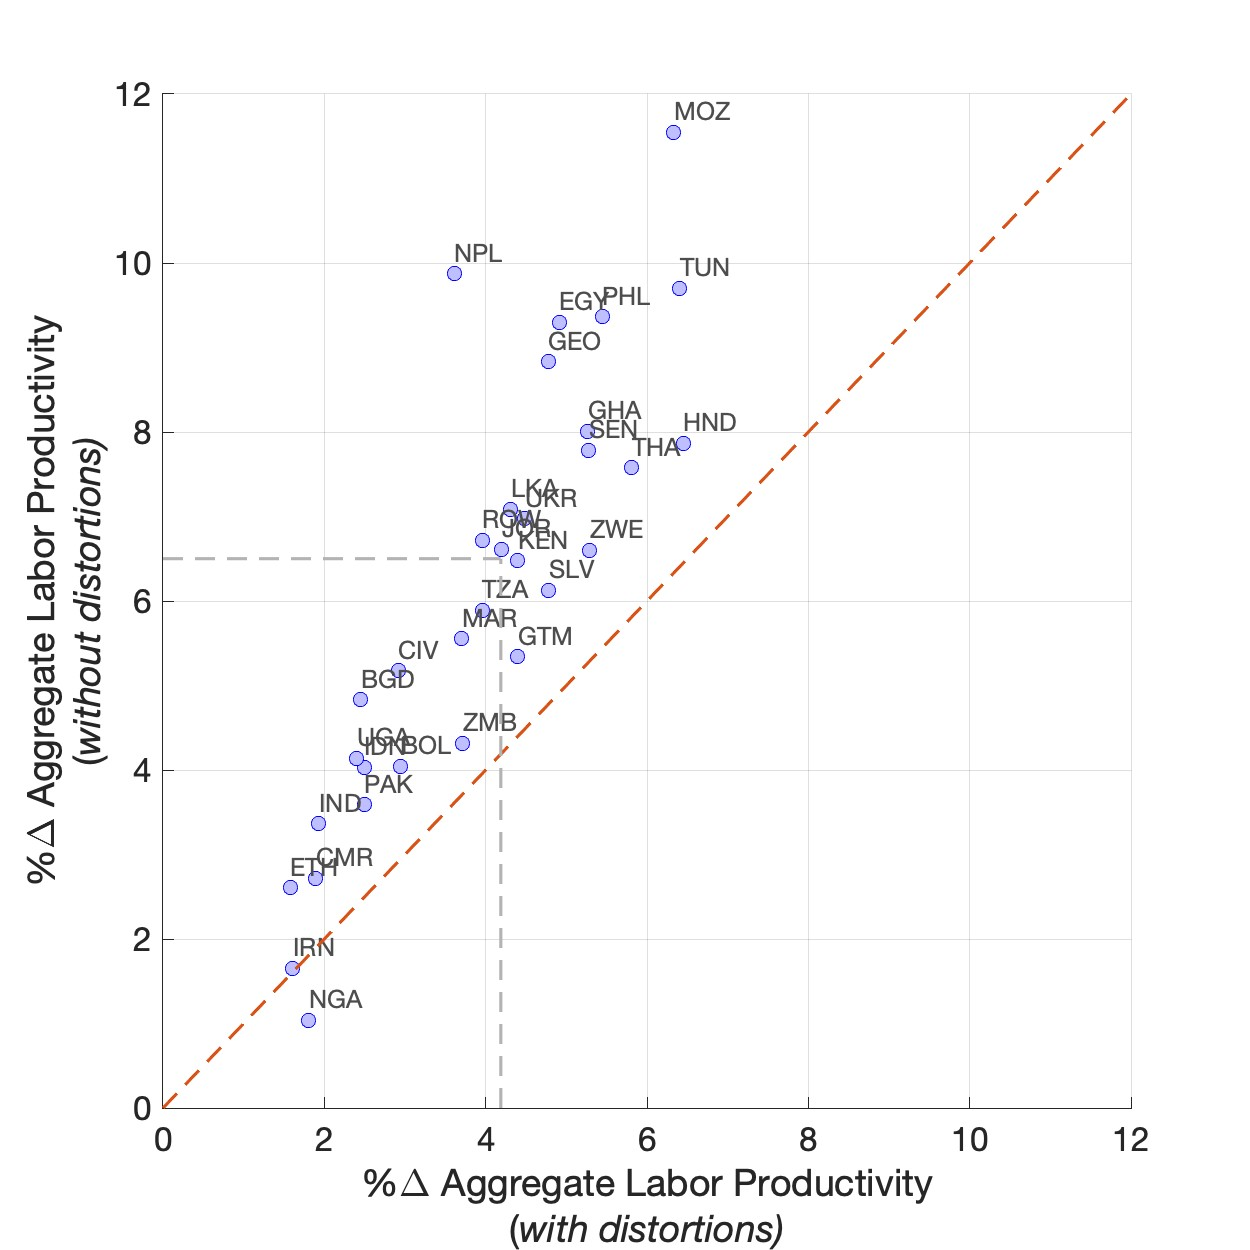
\includegraphics[scale=0.22]{fig/ALP}
\par\end{centering}
\textbf{\footnotesize{}Notes}{\footnotesize{}: This figure shows the
percentage change to aggregate labor productivity, defined by Equation
(\ref{eq:ALP_i}), among low-income countries in response to a 20\%
reduction in trade costs. The x-axis reports changes under the status
quo labor wedges, the y-axis reports changes under no labor wedges.}{\footnotesize\par}
\end{figure}


\section{Robustness Checks\label{subsec:Robustness}}

This section provides robustness checks based on alternative calibrations
of our model. First, we use information on formal versus informal
firms to assign them to modern and traditional types. Second, we relax
the assumption that factor intensities of modern and traditional technologies
are common across countries. Third, we experiment with alternative
values of the technology elasticity, $\theta$. Under these alternative
calibrations, we re-evaluate the labor productivity effects the trade
liberalization discussed in Section \ref{subsec:Productivity-Gains-Quantitative}.
In addition, this section documents additional empirical patterns
and estimates of labor intensity and wedges that support our analysis.

\subsection{Formal versus Informal\label{subsec:formal_vs_informal}}

We adopt here an alternative approach in which we classify firms in
the formal sector as modern and firms in the informal sector as traditional.
To do so, we bring in the special surveys from the WBES that record
firm-level data of the informal sector, the Informal Sector Enterprise
Survey (IFS). The surveys on informal firms, however, are available
only for 23 countries. Using this subset of countries, we estimate
labor intensities and wedges for formal and informal firms. For countries
in which this survey is not provided, we use the labor wedges from
our baseline calibration. To construct the share of firms and total
sales from the informal sector, we use data from \citet{schneider2007shadow},
discussed in \citet{la2008unofficial}. Appendix \ref{sec:apx_robustness}
provides additional details about the calibration of the model.

There is a large difference between the output elasticity of labor
between production technologies in the formal and informal sectors:
The output elasticity in the informal sector is 0.53 whereas in the
formal sector it is 0.39 (Appendix Figure \ref{fig:apx_alternative_procedures}).
In comparison, in our baseline analysis, the output elasticity was
0.39 in the traditional sector against 0.29 in the modern one. Turning
to labor market wedges, there is a substantial gap between the average
labor wedge in the formal sector (5.04) and that of the informal sector
(1.91).\footnote{In comparison, the average labor wedges in our main calibration were,
respectively, 2.28 and 3.69 for traditional and modern firms. That
is, the classification based on formal vs. informal divide reinforces
the main mechanism in our model as it generates even a larger gap
in labor wedges between the resulting two groups of firms. Yet, the
correlation between the labor wedges in our baseline analysis and
the ones obtained from the formal vs informal cut of the data is 0.83.} Importantly, the qualitative patterns that we documented in Section
2 continue to hold under this alternative classification. Simulating
the model under this alternative approach, our main quantitative result\textemdash that
trade liberalization has a larger impact on aggregate labor productivity
in efficient economies\textemdash is preserved, although the impact
becomes somewhat weaker quantitatively (Appendix Figure \ref{fig:robustness_trade_liberalization_apdx}).

\subsection{Heterogeneous Labor Elasticities across Countries\label{subsec:heterogeneous_labor_intensities}}

In our baseline analysis, we assumed that factor intensities of modern
and the traditional technologies were common across countries.\footnote{Two comments are in order regarding this assumption in our baseline
analysis. First, production technologies are still different across
firms in countries since TFPs vary by firms. Second, the analysis
still allows for cross-country differences in aggregate factor intensity
as such differences arise from endogenous share of firms that use
modern and traditional technologies.} Here, we relax this assumption. Because our dataset does not provide
us with a sufficient coverage of firms to estimate technology-specific
factor intensities separately for each country, as a middle ground,
we run our estimation for firms in low-income countries and separately
for middle- and high-income countries. This procedure delivers a (potentially)
different classification of firms into modern and traditional types,
and alternative estimates of output elasticity of labor and labor
market wedges.

The output elasticity of labor for each technology is quite comparable
between low-income countries and middle- and high-income countries:
for low-income countries, the output elasticity of labor in the traditional
technology is 0.38, whereas the corresponding elasticity for middle-
and high-income countries is 0.41 (Appendix Figure \ref{fig:apx_alternative_procedures}).
We find that in both groups of countries labor wedges are larger among
modern firms, relative to traditional ones, and this difference is
substantially larger among firms in low-income countries\textemdash consistent
with the pattern in Figure \ref{fig:fact_section2} presented earlier
in Section \ref{sec:motivating_evidence}. Simulating the model with
this calibration, we find results that are largely comparable to the
ones from our baseline analysis (Appendix Figure \ref{fig:robustness_trade_liberalization_apdx}).

\subsection{Alternative Values of the Technology Elasticity ($\theta$) \label{subsec:apx_alternative_thetas}}

We conduct two sets of exercises to demonstrate how predictions of
our model depend on the technology elasticity, $\theta$. First, Appendix
Figure \ref{fig: robustness - theta (appendix)} shows the results
from a 20\% reduction in trade costs for different values of $\theta$.
At a higher $\theta$, the model generates a considerably larger trade-induced
adoption of modern technologies. This is expected since a higher technology
elasticity implies a larger response when the returns to modern technologies
rise (as induced by an improvement in access to foreign intermediates).

However, the effect of the technology elasticity on aggregate labor
productivity is less pronounced. On the one hand, an expansion in
the use of modern technologies increases aggregate labor productivity.
On the other hand (and acting against this force), there is a dampening
effect on aggregate productivity because the infra-marginal managerial
capital that gets reallocated to the modern technology is less productive
than the existing managerial capital there. Numerically, as we increase
the technology elasticity, $\theta$, the relative strength of the
former force rises to a limited extent, increasing the impact on the
aggregate labor productivity to a modest degree.

Second, we redo our exercise in Section \ref{subsec:Productivity-Gains-Quantitative}
with two alternative values of the technology elasticity, $\theta=2$
and $\theta=9$ (our baseline calibration sets $\theta=4.5$). For
these two alternative calibrations, Panels (e)\textendash (h) in Appendix
Figure \ref{fig:robustness_trade_liberalization_apdx} show the impact
of the trade liberalization on aggregate labor productivity and real
wages with and without distortions, similar to our main exercise in
Section \ref{subsec:Productivity-Gains-Quantitative}. The resulting
outcomes remain to be similar both qualitatively and quantitatively
to our baseline results.

\subsection{Additional Evidence\label{subsec:Additional-Supporting-Evidence}}

To conclude, we present additional evidence based on the WBES that
bolster our quantitative approach.

First, we experiment with several alternative approaches for the estimation
of labor intensity and wedges. Specifically, we: \emph{(i)} estimate
labor intensity both by sector and technology type, as opposed to
only by technology, \emph{(ii)} allow for more than 2 technology types,
and \emph{(iii)} estimate labor intensity using different dependent
variables (either total sales or total costs) and different control
functions. Results are reported in Appendix Table \ref{tab:apx_labor_intensity_rob}
and Appendix Figures \ref{fig:fact_share_labor_technology} and \ref{fig:fact3_app}.
Reassuringly, across all different cuts and estimation approaches,
modern firms use labor less intensively than smaller ones, and are
subject to higher labor wedges.

Furthermore, we document three patterns using WBES surveys in which
firms are asked to report the obstacles they face in their businesses.
First, modern firms tend to report more severe obstacles due to taxes,
labor regulations and informal sectors relative to traditional firms,
but less so in high-income countries (Appendix Table \ref{tab:apx_direct_evidence}).
Second, across several different approaches for the estimation of
labor intensity and labor market distortions, modern firms face larger
(model-implied) distortions, and more so in low-income countries (Appendix
Table \ref{tab:apdx_labor_wedges_GDP}). Third, generally our estimates
of distortions are positively correlated with these direct measures
of obstacles across countries (Appendix Table \ref{tab:apx_labor_wedges_model_vs_data}).

\section{Conclusion\label{sec:Conclusion}}

In this paper, we studied how labor market imperfections distort firm-level
technology choices and alter the gains from trade. To do so, we introduced
labor market distortions and technology choices into a multi-country,
quantitative trade model. We provided analytical expressions highlighting
the mechanisms that drive the impact of trade liberalizations on aggregate
welfare and labor productivity. We compared the gains from trade in
our framework to the canonical ACR results, and employed counterfactual
simulations to study the implications of trade liberalization for
aggregate labor productivity, particularly in low-income countries.

Our findings indicates that the low adoption of modern technologies
despite globalization, a topic of much debate among researchers and
policymakers, can be partly attributed to labor market distortions.
Specifically, labor market distortions can substantially reduce the
potential labor productivity gains. This is an important result as
researchers have been particularly concerned about the implications
of technology upgrading for workers, given the stagnation of aggregate
labor productivity in parts of the developing world. Our results suggest
that reductions in labor market distortions, a ubiquitous feature
of developing economies, can substantially boost the labor productivity
gains from trade-led growth in modern technologies.

Our paper offers a few promising avenues for future research. First,
our framework could be extended to examine the \emph{distributional}
impacts of trade in distorted economies, for example, by bringing
in employee-employer matched data on different types of workers. Second,
our analysis can be extended to incorporate other forms of inefficiencies,
such as barriers that distort firms' choices of \emph{capital}. Lastly,
our current approach is agnostic about the specific institutional
mechanisms that generate labor market distortions. Future research
could consider \emph{endogenous distortions} that interact with technology
adoption, for example, by studying the impact of search frictions
in labor markets or the implications of moving firms out of informality.

\section*{References}

%\begin{btSect}[plainnat]{bibliography}
%\btPrintCited
%\end{btSect}

\bibliographystyle{apalike}
\bibliography{biblio}

\vspace{-2cm}


% \begin{btUnit}

\part{Appendices\vspace{-2cm}
}


\appendix
\onehalfspacing
\fontsize{11}{12}\selectfont 

\clearpage 

% Appendix tables -- fix to get hyperref correct 
%\newcounter{atable} 
%\addtocounter{atable}{0} 
%\renewcommand{\thetable}{A\arabic{atable}} 

\setcounter{table}{0} 

\renewcommand{\thetable}{A.\arabic{table}} 
\newcounter{atable} \addtocounter{atable}{0} 
\setcounter{figure}{0}

\renewcommand{\thefigure}{A.\arabic{figure}} 
\newcounter{afigure} \addtocounter{afigure}{0}
\numberwithin{equation}{section}

\pagenumbering{arabic}
\begin{center}
{\LARGE{}Online Appendices for ``Trade and Technology Adoption in
Distorted Economies''}{\LARGE\par}
\par\end{center}

\begin{center}
{\LARGE{}Not for Publication}{\LARGE\par}
\par\end{center}

\begin{center}
Farid Farrokhi, Ahmad Lashkaripour, and Heitor S. Pellegrina\blfootnote{Email: ffarrokh@purdue.edu, alashkar@indiana.edu, and hpelleg@nd.edu.}
\par\end{center}

\begin{flushright}
\mtcsetrules{parttoc}{off}
\tightmtctrue
\parttoc[n]
\onehalfspacing{\huge{}\newpage}{\huge\par}
\par\end{flushright}

\section{Derivations of Model Relationships and ALP\label{sec:Analytical-Results_apdx}}

This section presents, first, derivations that relate model-implied
revenue shares, labor shares, and the share of modern firms. We use
these relationships throughout the paper to derive several of our
expressions. In addition, we present a full derivation of our formula
for aggregate labor productivity.

\subsection{\label{subsec: Shares (Appendix)}Relationship between $\alpha$,
$\rho$, and $\ell$}

This appendix derives expressions for revenue shares ($\rho_{i,st}$)
and labor shares ($\ell_{i,st}$) as a function of $\alpha_{i,st}$,
which is the share of firms that chose technology $t$ in country
$i$\textendash industry $s$. To fix idea, we formally define the
aforementioned share variables. The labor shares are defined as follows
for various tiers of production (i.e., firm, technology, and industry)
\[
\ell_{i,st}\left(\omega\right)=\frac{L_{i,st}\left(\omega\right)}{L_{i}};\qquad\qquad\qquad\ell_{i,st}=\sum_{\omega\in\Omega_{i,st}}\ell_{i,st}\left(\omega\right);\qquad\qquad\qquad\ell_{i,s}=\sum_{t}\ell_{i,st}.
\]
We use $\rho$ to denote \emph{within-industry} revenue shares and
$r$ to denote industry-level revenue share. In particular, 
\[
\rho_{i,st}\left(\omega\right)=\frac{R_{i,s}\left(\omega\right)}{R_{i,s}};\qquad\qquad\qquad\rho_{i,st}=\int\rho_{i,st}\left(\omega\right)dF\left(\omega|\omega\in\Omega_{st}\right);\qquad\qquad\qquad r_{i,s}=\sum_{t}\rho_{i,st}
\]
where $R_{i,st}\left(\omega\right)\equiv p_{i,s}Q_{i,st}\left(\omega\right)$,
recall, denotes total revenues collected by firm $\omega$, with $R_{i,s}\equiv\sum_{t}\int_{\omega}R_{i,st}\left(\omega\right)dF\left(\omega|\omega\in\Omega_{st}\right)$
denoting industry-level revenues. Appealing to Equations (\ref{eq:R_ist})
and (\ref{eq:R_is}) we can derive the following relationship between
firm and sales shares:
\[
\begin{cases}
\alpha_{i,st}=\left(a_{i,st}h_{i,st}/\grave{\tau}_{i,st}^{L}\right)^{\theta}H_{i,s}^{-\theta}\\
p_{i,s}=\left(\frac{\grave{\tau}_{i,st}}{a_{i,st}h_{i,st}}\right)\alpha_{i,st}^{\frac{1-\theta}{\theta}}\gamma_{st}^{Z}\rho_{i,st}R_{i,s}
\end{cases}\qquad\Longrightarrow\qquad\frac{\alpha_{i,st}}{\alpha_{i,st'}}=\frac{\gamma_{st}^{Z}\rho_{i,st}}{\gamma_{st'}^{Z}\rho_{i,st'}}
\]
Combining the above equation with the adding up constraints, $\sum_{t}\rho_{i,st}=\sum_{t}\alpha_{i,st}=1$,
yields
\[
\rho_{i,st}=\frac{\frac{1}{\gamma_{st}^{Z}}\alpha_{i,st}}{\sum_{t'}\frac{1}{\gamma_{st'}^{Z}}\alpha_{i,st'}}=\frac{\Gamma_{is}^{Z}}{\gamma_{st}^{Z}}\alpha_{i,st},\qquad\text{where}\qquad\qquad\frac{1}{\Gamma_{is}^{Z}}=\sum_{t}\frac{1}{\gamma_{i,st}^{Z}}\alpha_{i,st}.
\]
To derive a relationship between labor shares and firm shares, we
appeal to the fact that gross labor cost equals a constant fraction,
$\gamma_{st}^{L}$, of gross revenues. In particular,
\[
\tau_{i,st}^{L}w_{i}\times\overbrace{L_{i,st}}^{\ell_{i,st}L_{i}}=\gamma_{st}^{L}\times\overbrace{Y_{i,st}}^{\rho_{i,st}Y_{i,s}}\qquad\Longrightarrow\qquad\frac{\ell_{i,st}}{\ell_{i,st'}}=\frac{\frac{\gamma_{st}^{L}}{\tau_{i,st}^{L}}\rho_{i,st}}{\frac{\gamma_{st'}^{L}}{\tau_{i,st'}^{L}}\rho_{i,st'}}=\frac{\frac{\gamma_{st}^{L}}{\tau_{i,st}^{L}\gamma_{st}^{Z}}\alpha_{i,st}}{\frac{\gamma_{st'}^{L}}{\tau_{i,st'}^{L}\gamma_{st'}^{Z}}\alpha_{i,st'}}.
\]
Combining this equation with the adding up constraints, $\sum_{t}\ell_{i,st}=\ell_{i,s}$
and $\sum_{t}\alpha_{i,st}=1$, delivers
\[
\ell_{i,st}=\frac{\frac{\gamma_{st}^{L}}{\tau_{i,st}^{L}\gamma_{st}^{Z}}\alpha_{i,st}}{\sum_{t'}\frac{\gamma_{st'}^{L}}{\tau_{i,st'}^{L}\gamma_{st'}^{Z}}\alpha_{i,st'}}\ell_{i,s};\qquad\qquad\qquad\qquad\ell_{i,st}=\frac{\frac{\gamma_{st}^{L}}{\tau_{i,st}^{L}}\rho_{i,st}}{\sum_{t'}\frac{\gamma_{st'}^{L}}{\tau_{i,st'}^{L}}\rho_{i,st'}}.
\]


\subsection{Aggregate Labor Productivity (ALP)\label{subsec:Aggregate-Labor-Productivity (Appendix)}}

We define Aggregate Labor Productivity (ALP) at the level of country-industry-technology
as output per worker there. Using the relationship between revenues
and quantities as well as the labor market clearing condition, it
follows that:

\begin{equation}
\text{ALP}_{i,st}\equiv\frac{Q_{i,st}}{L_{i,st}}=\frac{R_{i,st}/p_{is}}{\gamma_{i,st}^{L}/\tau_{i,st}^{L}\times R_{i,st}/w_{i}}=\frac{\tau_{i,st}^{L}}{\gamma_{i,st}^{L}}\times\frac{w_{i}}{p_{i,s}}\label{eq:ALP_ist_apdx}
\end{equation}
Similarly, ALP at the level of industry can be expressed as:
\begin{equation}
\text{ALP}{}_{i,s}\equiv\frac{Q_{i,s}}{L_{i,s}}=\frac{\sum_{t}R_{i,st}/p_{is}}{L_{i,s}}=\sum_{t}\left[\frac{L_{i,st}}{L_{i,s}}\times\text{ALP}_{i,st}\right]\label{eq:ALP_is_apdx}
\end{equation}
Lastly, we derive the expression for ALP at the level of country.
Here, we aggregate over industry-level output quantities using the
final consumption aggregator, $Q_{i}=\prod_{s}\left(Q_{i,s}\right)^{\beta_{i,s}}$.
Under this assumption, we have:

\begin{align}
\text{ALP}{}_{i}\equiv\frac{Q_{i}}{L_{i}} & =\frac{\prod_{s}\left(Q_{i,s}\right)^{\beta_{i,s}}}{L_{i}}\label{eq:ALP_i_apdx}\\
 & =\prod_{s}\left(\frac{L_{i,s}}{L_{i}}\times\frac{Q_{i,s}}{L_{i,s}}\right)^{\beta_{i,s}}\nonumber \\
 & =\prod_{s}\left(\frac{L_{i,s}}{L_{i}}\times\left[\sum_{t}\frac{L_{i,st}}{L_{i,s}}\times\text{ALP}_{i,st}\right]\right)^{\beta_{i,s}}\nonumber \\
 & =\left(\frac{w_{i}}{\prod_{s}p_{i,s}^{\beta_{i,s}}}\right)\times\prod_{s}\left[\sum_{t}\left(\ell_{i,st}\times\frac{\tau_{i,st}^{L}}{\gamma_{i,st}^{L}}\right)\right]^{\beta_{i,s}}\nonumber \\
 & =\left(\frac{w_{i}}{P_{i}}\right)\times\left[\prod_{s}\left(\pi_{ii,s}\right)^{\frac{\beta_{i,s}}{\sigma_{s}-1}}\right]\times\left[\prod_{s}\left(\sum_{t}\ell_{i,st}\times\frac{\tau_{i,st}^{L}}{\gamma_{i,st}^{L}}\right)^{\beta_{i,s}}\right]\nonumber 
\end{align}
where $\ell_{i,st}\equiv\frac{L_{i,st}}{L_{i}}$ and $\pi_{ii,s}$
is the domestic expenditure share. In the above, we use $P_{i,s}=p_{i,s}\left(\pi_{ii,s}\right)^{\frac{1}{\sigma_{s}-1}}$
and $P_{i}=\prod_{s}P_{i,s}^{\beta_{i,s}}.$

To establish the relationship between aggregate labor productivity
$\text{ALP}_{i}$ (Equation \ref{eq:ALP_i}) and welfare $W_{i}$
(Equation \ref{eq:W_i (Welfare)}), start from the third line of the
above derivation, and replace for $\text{ALP}_{i,st}=\frac{R_{i,st}}{p_{i,s}L_{i,st}},$
\begin{align*}
\text{ALP}_{i} & =\prod_{s}\left(\sum_{t}\frac{L_{i,st}}{L_{i}}\times\text{ALP}_{i,st}\right)^{\beta_{i,s}}=\prod_{s}\left(\sum_{t}\frac{1}{L_{i}}\times\frac{R_{i,st}}{p_{i,s}}\right)^{\beta_{i,s}}=\frac{1}{L_{i}}\prod_{s}\left(\frac{R_{i,s}}{p_{i,s}}\right)^{\beta_{i,s}}
\end{align*}

Denoting $Y_{i,s}$ as total value added and $\bar{\gamma}_{i,s}^{M}$
as the average cost share of intermediate inputs in country $i-$industry
$s$, using the relationship between producer and consumer prices
(as shown above), and definition of welfare $W_{i}=Y_{i}/P_{i}$,
we can express $\text{ALP}_{i}$ as:
\[
\text{ALP}_{i}=\left[\prod_{s}\left(\pi_{ii,s}\right)^{\frac{\beta_{i,s}}{\sigma_{s}-1}}\right]\times\left[\prod_{s}\left(\frac{\left(Y_{i,s}/Y_{i}\right)}{1-\bar{\gamma}_{i,s}^{M}}\right)^{\beta_{i,s}}\right]\times\left(\frac{W_{i}}{L_{i}}\right)
\]


\section{General Equilibrium in Changes \label{subsec:QGE (Appendix)}}

\subsection{Specifying the System of GE in Changes}

Consider a ``policy'' as a set of exogenous shocks to trade costs,
labor wedges, and productivities, $\mathscr{P}=\{\hat{d}_{ij,s},\hat{\tau}_{i,st}^{L},\hat{a}_{i,st}\}$.
Let $\mathscr{B}=\{\sigma,\theta,\pi_{ij,s},\alpha_{i,st},\gamma_{st}^{L},\gamma_{st}^{M},\gamma_{st}^{Z},\tau_{i,st}^{L},\phi_{i,\ell s},\beta_{i,s},w_{i}L_{i},R_{i,st},E_{i,s},Y_{i}\}$
denote the ``baseline'' values of the general equilibrium\textemdash i.e.,
the set of sufficient statistics. For any generic variable $x$ in
the baseline equilibrium, let $x^{\prime}$ be its corresponding value
in the counterfactual equilibrium, and $\hat{x}\equiv x^{\prime}/x$
denote its change from the baseline to the counterfactual equilibrium.
Given policy $\mathscr{P}$ and baseline values $\mathscr{B}$, the
following equations define general equilibrium in changes to trade
and technology shares, aggregate sales and expenditures, and prices
and wages, $\mathscr{E}\equiv\{\hat{\pi}_{ij,s},\hat{\alpha}_{i,st},\hat{R}_{i,st},\hat{E}_{i,s},\hat{Y}_{i},\hat{p}_{i,s},\hat{P}_{i,s},\hat{w}_{i}\}$.

The change to sales in country $i-$industry $s-$technology $t$
is:

\begin{equation}
\widehat{R}_{i,st}=\left(\widehat{a}_{i,st}\widehat{\widetilde{h}}_{i,st}/\widehat{p}_{i,s}\right)\times\left(\widehat{\alpha}_{i,st}\right)^{\frac{\theta-1}{\theta}},\label{eq:apdx_hat_R_ist}
\end{equation}
where the change to the share of firms in each technology type is
given by:

\begin{equation}
\widehat{\alpha}_{i,st}=\frac{\left(\widehat{a}_{i,st}\widehat{\widetilde{h}}_{i,st}\right)^{\theta}}{\sum_{t\in\mathbb{T}}\alpha_{i,st}\left(\widehat{a}_{i,st}\widehat{\widetilde{h}}_{i,st}\right)^{\theta}},\quad\mbox{where}\quad\widehat{a}_{i,st}=\left(\hat{A}_{i,st}\right)^{1/\gamma_{st}^{Z}};\label{eq:apdx_hat_alpha_ist}
\end{equation}
and the change to technology-specific return to managerial capital
is:

\begin{equation}
\widehat{\widetilde{h}}_{i,st}\equiv\left(\hat{\tau}_{i,st}^{L}\right)^{-\gamma_{st}^{L}/\gamma_{st}^{Z}}\underbrace{\left(\frac{\hat{\tau}_{i,st}^{L}\widehat{w}_{i}}{\widehat{p}_{i,s}}\right)^{-\gamma_{st}^{L}/\gamma_{st}^{Z}}\left(\frac{\widehat{m}_{i,st}}{\widehat{p}_{i,s}}\right)^{-\gamma_{st}^{M}/\gamma_{st}^{Z}}}_{\widehat{h}_{i,st}},\quad\mbox{where}\quad\widehat{m}_{i,st}=\prod_{\ell\in\mathbb{S}}\left(\widehat{P}_{i,\ell}\right)^{\phi_{i,\ell st}}.\label{eq:apdx_hat_h_ist}
\end{equation}
In turn, the change to the industry-level (consumer) price index equals:

\begin{equation}
\widehat{P}_{j,s}=\left[\sum_{i\in\mathbb{I}}\pi_{ij,s}\left(\widehat{d}_{ij,s}\widehat{p}_{i,s}\right)^{1-\sigma_{s}}\right]^{\frac{1}{1-\sigma_{s}}},\label{eq:apdx_hat_P_js}
\end{equation}
and the change to within-industry share of expenditure (trade share)
is:

\begin{equation}
\widehat{\pi}_{ij,s}=\frac{\left(\widehat{d}_{ij,s}\widehat{p}_{i,s}\right)^{1-\sigma_{s}}}{\left(\widehat{P}_{j,s}\right)^{1-\sigma_{s}}}.\label{eq:apdx_hat_pi_ijs}
\end{equation}
Lastly, the following four equations guarantee the market clearing
conditions and the accounting of general equilibrium. The labor market
clearing condition and the goods market clearing condition in the
counterfactual equilibrium must satisfy:

\begin{equation}
\widehat{w}_{i}w_{i}L_{i}=\left[\sum_{s,t}\frac{\gamma_{st}^{L}}{\hat{\tau}_{i,st}^{L}\tau_{i,st}^{L}}\widehat{R}_{i,st}R_{i,st}\right]\label{eq:apdx_hat_MCC Labor}
\end{equation}
\begin{equation}
\left(\sum_{t}\hat{R}_{i,st}R_{i,st}\right)=\sum_{j}\hat{\pi}_{ij,s}\pi_{ij,s}\hat{E}_{j,s}E_{j,s}\label{eq:apdx_hat_MCC Goods}
\end{equation}
The change to the industry-level gross expenditures and the total
national expenditure (nominal GDP) satisfy:

\begin{equation}
\widehat{E}_{i,s}E_{i,s}=\left[\beta_{i,s}\widehat{Y}_{i}Y_{i}+\sum_{t,\ell}\phi_{i,\ell}^{s}\gamma_{\ell t}^{M}\widehat{R}_{i,\ell t}R_{i,\ell t}\right]\label{eq:apdx_hat_E_is}
\end{equation}

\begin{equation}
\widehat{Y}_{i}Y_{i}=\sum_{s,t}\left(1-\gamma_{i,st}^{M}\right)\widehat{R}_{i,st}R_{i,st}\label{eq:apdx_hat_Y_i}
\end{equation}
We now turn to presenting the computational algorithm that we use
to simulate the general equilibrium of our model in response to counterfactual
policy shocks.

\subsection{Numerical Algorithm to Simulate the GE in Changes.}
\begin{enumerate}
\item Guess $\widehat{w}_{i}$ and $\widehat{p}_{i,s}$. (By the choice
of numeraire, here we impose that $\hat{w}_{i_{0}}=1$ for a reference
country $i_{0}$)
\item Calculate the change to industry-level price index, $\widehat{P}_{i,s}$,
according to Equation (\ref{eq:apdx_hat_P_js}).
\item Calculate the change to technology-level returns to managerial capital
according to Equation (\ref{eq:apdx_hat_h_ist}).
\item Calculate the change to trade shares, $\hat{\pi}_{ij,s}$, based on
Equation (\ref{eq:apdx_hat_pi_ijs}).
\item Calculate the change to technology shares, $\widehat{\alpha}_{i,st}$,
according to Equation (\ref{eq:apdx_hat_alpha_ist}).
\item Calculate the change to sales, $\hat{R}_{i,st}$, based on Equation
(\ref{eq:apdx_hat_R_ist}).
\item Calculate the change to national expenditure, $\hat{Y}_{i}$, based
on Equation (\ref{eq:apdx_hat_Y_i}).
\item Calculate the change to industry-level gross expenditures, $\widehat{E}_{i,s}$,
based on Equation (\ref{eq:apdx_hat_E_is}).
\item Update the change to wages and prices, based on market clearing conditions
(\ref{eq:apdx_hat_MCC Labor}) and (\ref{eq:apdx_hat_MCC Goods}),
\[
\left(\widehat{w}_{i}\right)^{new}=\frac{1}{w_{i}L_{i}}\left[\sum_{s,t}\frac{\gamma_{st}^{L}}{\hat{\tau}_{i,st}^{L}\tau_{i,st}^{L}}\widehat{R}_{i,st}R_{i,st}\right]
\]
\[
\left(\widehat{p}_{i,s}\right)^{new}=\frac{\sum_{j}\hat{\pi}_{ij,s}\pi_{ij,s}\hat{E}_{j,s}E_{j,s}}{\left(\sum_{t}\left(\hat{R}_{i,st}/\hat{p}_{i,st}\right)R_{i,st}\right)}
\]
If the $|\left(\widehat{w}_{i}\right)^{new}-\widehat{w}_{i}|>\epsilon$
and $|\left(\widehat{p}_{i,s}\right)^{new}-\widehat{p}_{i,s}|>\epsilon$,
for a sufficiently small tolerance $\epsilon$, then update: $\widehat{w}_{i}=\left(\widehat{w}_{i}\right)^{new}$
and $\hat{p}_{i,s}=\left(\widehat{p}_{i,s}\right)^{new}$, and normalize
the updated price and wage changes with respect to the wage change
in a reference country (whose labor serves as a numeraire), then go
to Step 2. Otherwise, the convergence is achieved.
\end{enumerate}

\section{\label{sec: Misallocation Formula (Appendix)}Derivation of The Welfare
Cost of Misallocation}

Consider the closed economy case of our model with one sector and
multiple technologies\textemdash noting that, with a reinterpretation
of indexes, our derivation extends to multiple sectors and technologies.
We, accordingly, condense the notation by dropping the industry subscript,
$s$, going forward. To provide closed-form formulas for the degree
of misallocation, we make two additional assumptions: First, we assume
that production employs only primary factors of production\textemdash namely,
labor and managerial capital. Second, we assume that the labor intensity
parameter, $\gamma_{i,t}^{L}$, is common across technologies. All
in all, we consider a closed economy where production can be conducted
under multiple technologies with different labor input wedges, with
firms having the ability to choose and adjust their preferred technology.

\paragraph*{Intermediate Definitions.}

The efficient allocation in this stylized version of our model is
achieved if labor input wedges and the revenue associated with them
are eliminated from the economy\textemdash which is akin to analyzing
the following shock:
\[
\hat{\tau}_{i,t}^{L}=\frac{1}{\tau_{i,t}^{L}};\qquad\qquad\forall t\in\mathbb{T}.
\]
Let $\hat{W}_{i}\left(\hat{\boldsymbol{\tau}}_{i}\right)$ denote
the resulting welfare change from the wedge reduction shock, $\hat{\boldsymbol{\tau}}_{i}\equiv\left\{ \tau_{i,t}^{L}\right\} $.
We define the \emph{degree of misallocation} ($\mathcal{D}_{i}$)
as the welfare distance between the decentralized (i.e, misallocated)
and the efficient economies. Namely,
\[
\mathcal{D}_{i}\equiv\log\hat{W}_{i}\left(\hat{\boldsymbol{\tau}}_{i}\right)=\log\hat{Y}_{i}\left(\hat{\boldsymbol{\tau}}_{i}\right)-\log\hat{P}_{i}\left(\hat{\boldsymbol{\tau}}_{i}\right).
\]


\paragraph*{The Change in Technology Composition.}

Considering our assumption that $\gamma_{i,t}^{L}=\gamma_{i,t'}^{L}=\gamma_{i}^{L}$
and $\gamma_{i,t}^{Z}=\gamma_{i,t'}^{Z}=\gamma_{i}^{Z}$ for all $t$
and $t'$, we can specify the change in the share of firms choosing
technology $t$ as
\[
\hat{\alpha}_{i,t}=\frac{\left(\hat{\tau}_{i,t}^{L}\right)^{-\frac{\gamma_{i}^{L}}{\gamma_{i}^{Z}}\theta}}{\sum_{t'}\alpha_{i,t'}\left(\hat{\tau}_{i,t'}^{L}\right)^{-\frac{\gamma_{i}^{L}}{\gamma_{i}^{Z}}\theta}}=\frac{\left(\tau_{i,t}^{L}\right)^{\frac{\gamma_{i}^{L}}{\gamma_{i}^{Z}}\theta}}{\sum_{t'}\alpha_{i,t'}\left(\tau_{i,t'}^{L}\right)^{\frac{\gamma_{i}^{L}}{\gamma_{i}^{Z}}\theta}}.
\]
Appealing to the above expression, we can characterize the change
in technology-level employment shares. For this, we invoke the relationships
derived in Appendix \ref{subsec: Shares (Appendix)} to arrive at
\begin{equation}
\rho_{i,t}=\alpha_{i,t};\qquad\qquad\qquad\ell_{i,t}=\frac{\frac{1}{\tau_{i,t}^{L}}\alpha_{i,t}}{\sum_{t'}\frac{1}{\tau_{i,t'}^{L}}\alpha_{i,t'}};\qquad\qquad\qquad\alpha_{i,t}=\frac{\tau_{i,t}^{L}\ell_{i,t}}{\sum_{t'}\tau_{i,t'}^{L}\ell_{i,t'}}.\label{eq: shares (misallocation appendix)}
\end{equation}
Notice that in the efficient, wedge-free equilibrium, employment and
revenue shares exactly coincide with firm shares (i.e., $\ell'_{i,t}=\rho'_{i,t}=\alpha'{}_{i,t}$),
yielding the following expression for technology-level employment
shares in the counterfactual wedge-free equilibrium:
\begin{align*}
\ell'_{i,t} & =\alpha'_{i,t}=\frac{\alpha_{i,t}\left(\tau_{i,t}^{L}\right)^{\frac{\gamma_{i}^{L}}{\gamma_{i}^{Z}}\theta}}{\sum_{t'}\alpha_{i,t'}\left(\tau_{i,t'}^{L}\right)^{\frac{\gamma_{i}^{L}}{1-\gamma_{i}^{L}}\theta}}.\\
 & =\frac{\alpha_{i,t}\left(\tau_{i,t}^{L}\right)^{\frac{\gamma_{i}^{L}}{\gamma_{i}^{Z}}\theta}}{\sum_{t'}\alpha_{i,t'}\left(\tau_{i,t'}^{L}\right)^{\frac{\gamma_{i}^{L}}{\gamma_{i}^{Z}}\theta}}=\frac{\tau_{i,t}^{L}\ell_{i,t}\left(\tau_{i,t}^{L}\right)^{\frac{\gamma_{i}^{L}}{\gamma_{i}^{Z}}\theta}}{\sum_{t'}\tau_{i,t'}^{L}\ell_{i,t'}\left(\tau_{i,t'}^{L}\right)^{\frac{\gamma_{i}^{L}}{\gamma_{i}^{Z}}\theta}}.
\end{align*}


\paragraph*{The Change in Nominal Income.}

In the decentralized (baseline) economy, nominal income in country
$i$ is the sum of wage income, managerial rents, and wedge revenues\textemdash i.e.,
$Y_{i}=w_{i}L_{i}+\Pi_{i}+T_{i}$. Noting that $w_{i}L_{i}+T_{i}=\sum_{t}\tau_{i,t}^{L}w_{i}L_{i,t}$
and that by cost minimization, $\Pi_{i}=\sum_{t}\frac{\gamma_{i}^{Z}}{\gamma_{i}^{L}}\tau_{i,t}^{L}w_{i}L_{i,t}$,
we can specify the nominal income in the baseline economy as
\begin{align*}
Y_{i} & =\sum_{t}\left[\left(\tau_{i,t}^{L}+\frac{\Pi_{i,t}}{w_{i}L_{i,t}}\right)\frac{L_{i,t}}{L_{i}}\right]w_{i}L_{i}\\
 & =\sum_{t}\left[\tau_{i,t}^{L}\left(1+\frac{\gamma_{i}^{Z}}{\gamma_{i}^{L}}\right)\frac{L_{i,t}}{L_{i}}\right]w_{i}L_{i}=\sum_{t}\left[\frac{\tau_{i,t}^{L}}{\gamma_{i}^{L}}\ell_{i,t}\right]w_{i}L_{i}.
\end{align*}
Invoking the same logic, nominal income in the efficient (counterfactual)
economy is $Y'_{i}=\sum_{t}\left[\frac{1}{\gamma_{i}^{L}}\ell'_{i,t}\right]w'_{i}L_{i}$.
Combining the expressions for $Y_{i}$ and $Y'_{i}$ and assigning
labor in country $i$ as the numeraire ($w'_{i}=w_{i}=1$) deliver
the following expression for the change in nominal income in country
$i$:
\[
\hat{Y}_{i}=\frac{\frac{1}{\gamma_{i}^{L}}\sum_{t}\left[\ell'_{i,t}\right]w_{i}'L_{i}}{\frac{1}{\gamma_{i}^{L}}\sum_{t}\left[\tau_{i,t}^{L}\ell_{i,t}\right]w_{i}L_{i}}=\frac{1}{\sum_{t}\left[\tau_{i,t}^{L}\ell_{i,t}\right]}.
\]
Finally, appealing to our short-hand notation for weighted means,
$\mathbb{E}_{\ell}\left[\tau_{i,t}^{L}\right]=\sum_{t}\left[\tau_{i,t}^{L}\ell_{i,t}\right]$,
we can express the change in log income as:
\begin{equation}
\hat{Y}_{i}\equiv\mathbb{E}_{\ell}\left[\tau_{i,t}^{L}\right]^{-1}\label{eq: log_Y_hat (appendix)}
\end{equation}


\paragraph*{The Change in Consumer Prices.}

Following Equation (\ref{eq:R_is}) in Section \ref{sec:Model}, the
change in the competitive price of goods produced via technology $t$
is
\begin{equation}
\hat{p}_{i}=\hat{Y}_{i}\times\left(\hat{H}_{i}\right)^{-1},\label{eq: p_i_hat (appendix)}
\end{equation}
where the above equation uses two features of our stylized model:
First, $\hat{\Gamma}_{i}^{Z}=1$, since factor intensities are the
same across technologies. Second, gross output, $R_{i}$, equals value
added, $Y_{i}$, since no intermediate inputs are used in production\textemdash and,
hence, in a one-sector economy $R_{i}=Y_{i}$ delivers national income.
By choice of numeraire, $\hat{w}_{i}=1$, and using Equation (\ref{eq: alpha_ist}),
we can express the change in $H_{i}$ as:\vspace*{-0.15in}
\[
\hat{H}_{i}=\sum_{t}\left[\alpha_{i,t}\left(\hat{p}_{i}/\hat{\tau}_{i,t}^{L}\right)^{\frac{\gamma_{i}^{L}}{\gamma_{i}^{Z}}\theta}\right]^{\frac{1}{\theta}}=\left(\hat{p}_{i}\right)^{\frac{\gamma_{i}^{L}}{\gamma_{i}^{Z}}}\sum_{t}\left[\alpha_{i,t}\left(\tau_{i,t}^{L}\right)^{\frac{\gamma_{i}^{L}}{\gamma_{i}^{Z}}\theta}\right]^{\frac{1}{\theta}}
\]
Plugging the above expression back into Equation (\ref{eq: p_i_hat (appendix)})
yields\vspace*{-0.15in}
\[
\hat{p}_{i}=\left[\sum_{t}\alpha_{i,t}\left(\tau_{i,t}^{L}\right)^{\frac{\gamma_{i}^{L}}{\gamma_{i}^{Z}}\theta}\right]^{-\frac{\gamma_{i}^{Z}}{\theta}}\left(\hat{Y_{i}}\right)^{\gamma_{i}^{Z}}.
\]
Using our short-hand notation for means, whereby $\mathbb{E}_{\alpha}\left[\left(\tau_{i,t}^{L}\right)^{\frac{\gamma_{i}^{L}}{\gamma_{i}^{Z}}\theta}\right]=\sum_{t'}\left[\alpha_{i,t'}\left(\tau_{i,t'}^{L}\right)^{\frac{\gamma_{i}^{L}\theta}{\gamma_{i}^{Z}}}\right]$
and noting that $\hat{Y_{i}}=\mathbb{E}_{\ell}\left[\tau_{i,t}^{L}\right]^{-1}$
(Equation (\ref{eq: log_Y_hat (appendix)})), we get\vspace*{-0.15in}
\[
\hat{p}_{i}=\mathbb{E}_{\alpha}\left[\left(\tau_{i,t}^{L}\right)^{\frac{\gamma_{i}^{L}}{\gamma_{i}^{Z}}\theta}\right]^{-\frac{\gamma_{i}^{Z}}{\theta}}\times\mathbb{E}_{\ell}\left[\tau_{i,t}^{L}\right]^{-\gamma_{i}^{Z}},
\]
where the first mean on the right-hand side can be converted from
an $\alpha$-weighted mean to an $\ell$-weighted mean by noticing
that $\alpha_{i,t}=\tau_{i,t}\ell_{i,t}/\mathbb{E}_{\ell}\left[\tau_{i,t}\right]$
. Specifically,
\[
\mathbb{E}_{\alpha}\left[\left(\tau_{i,t}^{L}\right)^{\frac{\gamma_{i}^{L}}{\gamma_{i}^{Z}}\theta}\right]^{-\frac{\gamma_{i}^{Z}}{\theta}}=\mathbb{E}_{\ell}\left[\left(\tau_{i,t}^{L}\right)^{1+\frac{\gamma_{i}^{L}}{\gamma_{i}^{Z}}\theta}\right]^{-\frac{\gamma_{i}^{Z}}{\theta}}\mathbb{E}_{\ell}\left[\tau_{i,t}^{L}\right]^{\frac{\gamma_{i}^{Z}}{\theta}},
\]
which when plugged into our last expression for $\hat{p}_{i}$, yields\vspace*{-0.15in}
\begin{align}
\hat{p}_{i} & =\left(\mathbb{E}_{\ell}\left[\left(\tau_{i,t}^{L}\right)^{1+\frac{\gamma_{i}^{L}}{\gamma_{i}^{Z}}\theta}\right]\times\mathbb{E}_{\ell}\left[\tau_{i,t}^{L}\right]^{\theta-1}\right)^{-\frac{\gamma_{i}^{Z}}{\theta}}.\label{eq: log_P_hat (Appendix)}
\end{align}


\paragraph*{Assembling the Pieces Together.}

The final step collects the expressions for $\hat{Y}_{i}$ (Equation
(\ref{eq: log_Y_hat (appendix)})) and $\hat{p}_{i}$ (Equation (\ref{eq: log_P_hat (Appendix)})),
to calculate the degree of misallocation, $\mathcal{D}_{i}=\log\hat{Y}_{i}-\log\hat{P}_{i}$
. Doing so and rearranging the terms delivers,\vspace*{-0.15in}
\begin{align*}
\frac{\hat{Y}_{i}}{\hat{p}_{i}} & =\frac{1}{\mathbb{E}_{\ell}\left[\tau_{i,t}^{L}\right]}\left(\mathbb{E}_{\ell}\left[\left(\tau_{i,t}^{L}\right)^{1+\frac{\gamma_{i}^{L}}{\gamma_{i}^{Z}}\theta}\right]\times\mathbb{E}_{\ell}\left[\tau_{i,t}^{L}\right]^{\theta-1}\right)^{\frac{\gamma_{i}^{Z}}{\theta}}\\
 & =\left(\frac{\mathbb{E}_{\ell}\left[\left(\tau_{i,t}^{L}\right)^{1+\frac{\gamma_{i}^{L}}{\gamma_{i}^{Z}}\theta}\right]}{\mathbb{E}_{\ell}\left[\tau_{i,t}^{L}\right]^{1+\frac{\gamma_{i}^{L}}{\gamma_{i}^{Z}}\theta}}\right)^{\frac{\gamma_{i}^{Z}}{\theta}}=\ \mathbb{E}_{\ell}\left[\left(\tilde{\tau}_{i,t}^{L}\right)^{1+\frac{\gamma_{i}^{L}}{\gamma_{i}^{Z}}\theta}\right]^{\frac{\gamma_{i}^{Z}}{\theta}},
\end{align*}
where, recall that, $\tilde{\tau}_{i,t}\equiv\tau_{i,t}/\mathbb{E}_{\ell}[\tau_{i,t}]$.

Next, we reintroduce the sector subscript, $s$, for consistency in
notation, implicitly assuming that all sectors are symmetric. We also
substitute $\gamma_{i}^{L}$ and $\gamma_{i}^{Z}$ with our notation
for average input intensities, $\bar{\gamma}_{i}^{L}$, and $\bar{\gamma}_{i}^{Z}$\textemdash noting
that the average input intensities are the same as $\gamma_{i}^{L}$
and $\gamma_{i}^{Z}$ when sectors are symmetric. With these amendments
to the notation, we get the following expression for the welfare cost
of misallocation:
\begin{equation}
\mathcal{D}_{i}=\mathbb{E}_{\ell}\left[\left(\tilde{\tau}_{i,st}^{L}\right)^{1+\frac{\bar{\gamma}_{i}^{L}}{\bar{\gamma}_{i}^{Z}}\theta}\right]^{\frac{\bar{\gamma}_{i}^{Z}}{\theta}}.\label{eq: D_i exact formula (appendix)}
\end{equation}
Later, we invoke this formula to characterize the cost of misallocation
in the presence of multiple \emph{asymmetric} sectors that differ
in their factor intensities. Before that, we provide a first-order
approximation for $\mathcal{D}_{i}$ to elucidate the determinants
of misallocation.

\paragraph*{Approximate Formula.}

Next, we derive a simple approximation for $\mathcal{D}_{i}$ using
Taylor's Theorem. To this end, we construct the Taylor expansion of
the following function,
\[
f\left(\left\{ \tilde{\tau}_{i,st}^{L}\right\} _{t}\right)=\mathbb{E}_{\ell}\left[\left(\tilde{\tau}_{i,st}^{L}\right)^{1+\frac{\bar{\gamma}_{i}^{L}}{\bar{\gamma}_{i}^{Z}}\theta}\right],
\]
 around $\left\{ \tilde{\tau}_{i,st}^{L}\right\} =\left\{ 1,...,1\right\} $,
which delivers the following second-order approximation
\[
\mathbb{E}_{\ell}\left[\left(\tilde{\tau}_{i,st}^{L}\right)^{1+\frac{\bar{\gamma}_{i}^{L}}{\bar{\gamma}_{i}^{Z}}\theta}\right]\approx1+\left(1+\frac{\bar{\gamma}_{i}^{L}}{\bar{\gamma}_{i}^{Z}}\theta\right)\mathbb{E}_{\ell}\left[\tilde{\tau}_{i,st}^{L}-1\right]+\frac{1}{2}\left(1+\frac{\bar{\gamma}_{i}^{L}}{\bar{\gamma}_{i}^{Z}}\theta\right)\frac{\bar{\gamma}_{i}^{L}}{\bar{\gamma}_{i}^{Z}}\theta\mathbb{E}_{\ell}\left[\left(\tilde{\tau}_{i,st}^{L}-1\right)^{2}\right]
\]
Notice that $\mathbb{E}_{\ell}\left[\tilde{\tau}_{i,st}^{L}\right]=1$
since $\tilde{\tau}_{i,st}\equiv\tau_{i,st}/\mathbb{E}_{\ell}\left[\tau_{i,st}^{L}\right]$.
Also, the second term on the right-hand is zero by definition of the
mean and the last term is simply the variance of $\left\{ \tilde{\tau}_{i,st}^{L}\right\} _{t}$,
which we denote by $\text{Var}_{\ell}\left[\tilde{\tau}_{i,st}^{L}\right]$.
Considering these points we can simplify the above approximation as
\begin{equation}
\mathbb{E}_{\ell}\left[\left(\tilde{\tau}_{i,st}^{L}\right)^{1+\frac{\bar{\gamma}_{i}^{L}}{\bar{\gamma}_{i}^{Z}}\theta}\right]\approx1+\frac{1}{2}\left(1+\frac{\bar{\gamma}_{i}^{L}}{\bar{\gamma}_{i}^{Z}}\theta\right)\frac{\bar{\gamma}_{i}^{L}}{\bar{\gamma}_{i}^{Z}}\theta\text{\ensuremath{\text{Var}_{\ell}\left[\tilde{\tau}_{i,st}^{L}\right]}}.\label{eq: approximation 1 (appendix)}
\end{equation}
Plugging the above approximation back into Equation \ref{eq: D_i exact formula (appendix)}
and noting that $\log\left(1+x\right)\approx x$ when $x\approx0$,
we get
\[
\mathcal{D}_{i}\approx\frac{\bar{\gamma}_{i}^{L}}{2}\left(1+\frac{\bar{\gamma}_{i}^{L}}{\bar{\gamma}_{i}^{Z}}\theta\right)\text{\ensuremath{\text{Var}_{\ell}\left[\tilde{\tau}_{i,st}^{L}\right]}}.
\]


\subsection{Cost of Misallocation with Multiple Sectors}

Next, we consider an economy with multiple sectors that differ in
their labor intensities. The change in nominal income is still given
by $\hat{Y}_{i}=\mathbb{E}_{\ell}\left[\tau_{i,st}^{L}\right]^{-1}$.
Following our earlier derivations, the change in sector-level prices
are given by\vspace*{-0.15in}
\[
\hat{p}_{i,s}=\left[\sum_{t}\alpha_{i,st}\left(\tau_{i,st}^{L}\right)^{\frac{\bar{\gamma}_{i,s}^{L}}{\bar{\gamma}_{i,s}^{Z}}\theta}\right]^{-\frac{\bar{\gamma}_{i,s}^{Z}}{\theta}}\left(\hat{Y_{i}}\right)^{\bar{\gamma}_{i,s}^{Z}},
\]
which, considering that $\hat{Y}_{i}=\mathbb{E}_{\ell}\left[\tau_{i,st}^{L}\right]^{-1}$
and our notation for the mean operator, yields\vspace*{-0.15in}
\[
\frac{\hat{Y}_{i}}{\hat{p}_{i,s}}=\mathbb{E}_{\alpha,s}\left[\left(\tau_{i,st}^{L}\right)^{\frac{\bar{\gamma}_{i,s}^{L}}{\bar{\gamma}_{i,s}^{Z}}\theta}\right]^{\frac{\bar{\gamma}_{i,s}^{Z}}{\theta}}\mathbb{E}_{\ell}\left[\tau_{i,st}^{L}\right]^{\bar{\gamma}_{i,s}^{Z}-1}.
\]
Notice that with multiple sectors $\alpha_{i,st}=\tau_{i,st}\ell_{i,st}/\mathbb{E}_{\ell,s}\left[\tau_{i,st}^{L}\right]$,
where $\mathbb{E}_{\ell,s}\left[.\right]$ denotes the within-industry
mean weighted by industry $s$ employment shares. Appealing to the
point, we can re-write the first mean on the right-hand side of the
above equation as\vspace*{-0.15in}
\begin{align*}
\mathbb{E}_{\alpha,s}\left[\left(\tau_{i,st}^{L}\right)^{\frac{\bar{\gamma}_{i,s}^{L}}{\bar{\gamma}_{i,s}^{Z}}\theta}\right]^{\frac{\bar{\gamma}_{i,s}^{Z}}{\theta}} & =\mathbb{E}_{\ell}\left[\left(\frac{\tau_{i,t}^{L}}{\mathbb{E}_{\ell,s}\left[\tau_{i,st}^{L}\right]}\right)^{1+\frac{\bar{\gamma}_{i,s}^{L}}{\bar{\gamma}_{i,s}^{Z}}\theta}\right]^{-\frac{\bar{\gamma}_{i,s}^{Z}}{\theta}}\mathbb{E}_{\ell,s}\left[\tau_{i,st}^{L}\right]^{-\bar{\gamma}_{i,s}^{L}}.
\end{align*}
Combining the above two equations, derivers the following expression
for the change in real income with respect to industry $s$ goods:\vspace*{-0.15in}
\[
\frac{\hat{Y}_{i}}{\hat{p}_{i,s}}=\left(\frac{\mathbb{E}_{\ell,s}\left[\tau_{i,st}^{L}\right]}{\mathbb{E}_{\ell}\left[\tau_{i,st}^{L}\right]}\right)^{\bar{\gamma}_{i,s}^{L}}\mathbb{E}_{\ell,s}\left[\left(\frac{\tau_{i,st}^{L}}{\mathbb{E}_{\ell,s}\left[\tau_{i,st}^{L}\right]}\right)^{1+\frac{\bar{\gamma}_{i,s}^{L}}{\bar{\gamma}_{i,s}^{Z}}\theta}\right]^{-\frac{\bar{\gamma}_{i,s}^{Z}}{\theta}}.
\]
To make the notation more compact, redefine the normalized wedges
at the technology and industry levels as\vspace*{-0.1in}
\[
\tilde{\tau}_{i,st}=\frac{\tau_{i,st}}{\mathbb{E}_{\ell}\left[\tau_{i,st}^{L}\right]};\qquad\qquad\qquad\qquad\mathcal{\widetilde{T}}_{i,s}^{L}\equiv\frac{\mathbb{E}_{\ell,s}\left[\tau_{i,st}^{L}\right]}{\mathbb{E}_{\ell}\left[\tau_{i,st}^{L}\right]}.
\]
Finally, given that preferences are Cobb-Douglas across industries
$\mathcal{D}_{i}=\sum_{s}e_{i,s}\log\left(\frac{\hat{Y}_{i}}{\hat{p}_{i,s}}\right)$,
which delivers the following equation for the welfare cost of misallocation
in a multi-sector model:
\[
\mathcal{D}_{i}=\log\sum\left[e_{i,s}\left(\bar{\gamma}_{i,s}^{L}\log\left(\mathcal{\tilde{T}}_{i,s}^{L}\right)+\frac{\bar{\gamma}_{i,s}^{Z}}{\theta}\log\mathbb{E}_{\ell}\left[\left(\tilde{\tau}_{i,st}^{L}\right)^{1+\frac{\bar{\gamma}_{i,s}^{L}}{\bar{\gamma}_{i,s}^{Z}}\theta}\right]\right)\right].
\]


\section{Derivations of Trade Effects on Welfare and Labor Productivity\label{sec:Welfare-and-Productivity-Derivations (appendix)}}

In this section, we derive the equations presented in Section \ref{subsec:Decomposing-Welfare-Using-Ex-Ante-Gains-Thoery}
of the paper, which specify the impacts of trade on welfare and the
labor productivity gains. We first employ the exact hat algebra to
derive exact welfare formulas. Moreover, to draw additional insight
into the mechanisms behind welfare effects, we also produce local
approximations from our exact formulas.

\subsection{Exact Changes to Income Levels and Prices}

For any generic variable $x$ in the baseline equilibrium let $x'$
be the corresponding value in the counterfactual equilibrium, with
the hat variable denoted by $\hat{x}\equiv x'/x$. Consider a set
of shocks to trade costs, $\left\{ \hat{d}_{ij,k}\right\} $, and
labor wedges, $\left\{ \hat{\tau}_{i,st}^{L}\right\} $. The welfare
impact of these shocks can be written as the change in national income
divided by the change in the final consumer price index,
\[
\hat{W}_{i}=\frac{\hat{Y}_{i}}{\hat{P}_{i}}
\]
Similarly, the change to the real wage is given by:
\[
\hat{W}_{i}^{L}=\frac{\hat{w}_{i}}{\hat{P}_{i}}
\]

We now turn to characterizing the change to income levels, wage bills,
and prices.

\paragraph{Change in Income.}

Recall that national income is the sum of net wage payments, the revenue
associate with labor wedges, and rents accruing to managerial capital.
Namely, $E_{i}=w_{i}L_{i}+T_{i}+\Pi_{i}$, where $T_{i}\equiv\sum\left[\left(\tau_{i,st}^{L}-1\right)w_{i}L_{i,s}\right]$
is the revenue from wedges and $\Pi_{i}\equiv\sum_{s,t,\omega}\Pi_{i,st}\left(\omega\right)$
is the sum of managerial rents. Since $w_{i}L_{i}+T_{i}=\sum_{s}\sum_{t}\left[\tau_{i,st}^{L}\ell_{i,st}\right]w_{i}L_{i}$
and $\Pi_{i}=\frac{\gamma_{st}^{Z}}{\gamma_{st}^{L}}\left(w_{i}L_{i}+T_{i}\right)$,
we can express country $i$'s level of income as:
\[
Y_{i}=\sum_{s,t}\left(1+\frac{\gamma_{st}^{Z}}{\gamma_{st}^{L}}\right)\tau_{i,st}\ell_{is,t}w_{i}L_{i},
\]
where $\ell_{i,st}\equiv L_{i,st}/L_{i}$. Therefore, the change to
income can be expressed as:
\begin{equation}
\hat{Y}_{i}=\sum_{s,t}\left[y_{i,st}\hat{\tau}_{i,st}\hat{\ell}_{is,t}\right]\hat{w}_{i},\label{eq:hat_Y_i_apdx}
\end{equation}
where $y_{i,st}$ is the share of income in country $i$ that is generated
in industry $s-$technology $t$,

\begin{equation}
y_{i,st}\equiv\frac{Y_{i,st}}{Y_{i}}=\frac{\left(1+\frac{\gamma_{st}^{Z}}{\gamma_{st}^{L}}\right)\tau_{i,st}\ell_{i,st}}{\sum_{s',t'}\left(1+\frac{\gamma_{s't'}^{Z}}{\gamma_{s't'}^{L}}\right)\tau_{i,s't'}\ell_{i,s't'}}\label{eq:y_ist_apdx}
\end{equation}


\paragraph*{Change in Prices.}

Using Equation (\ref{eq:R_ist}) from the main text, the change to
output (sales) from country $i-$industry $s-$technology $t$ , $\hat{R}_{i,st}$,
equals:
\begin{equation}
\hat{R}_{i,st}=\hat{p}_{i,s}\hat{h}_{i,st}\left(\widehat{\alpha}_{i,st}\right)^{\frac{\theta-1}{\theta}}\label{eq:hat_R_ist_apdx}
\end{equation}
Moreover, it follows from Equation (\ref{eq: alpha_ist}) that the
change to returns per dollar of output in country $i-$industry $s-$technology
$t$, $\hat{h}_{is,t}$, is given by: 
\begin{equation}
\widehat{h}_{i,st}\equiv\left(\frac{\hat{\tau}_{i,st}^{L}\widehat{w}_{i}}{\widehat{p}_{i,s}}\right)^{-\gamma_{st}^{L}/\gamma_{st}^{Z}}\left(\frac{\widehat{m}_{i,st}}{\widehat{p}_{i,s}}\right)^{-\gamma_{st}^{M}/\gamma_{st}^{Z}}\label{eq:hat_h_ist_apdx}
\end{equation}
Replacing $\widehat{h}_{i,st}$ from Equation (\ref{eq:hat_h_ist_apdx})
into Equation (\ref{eq:hat_R_ist_apdx}) delivers the following expression
for $\hat{R}_{i,s,t}$:
\[
\hat{R}_{i,st}=\left(\hat{p}_{i,s}\right)^{\frac{1}{\gamma_{st}^{Z}}}\left(\hat{\tau}_{i,st}^{L}\right)^{-\frac{\gamma_{st}^{L}}{\gamma_{st}^{Z}}}\left(\hat{w}_{i}\right)^{-\frac{\gamma_{st}^{L}}{\gamma_{st}^{Z}}}\left(\hat{m}_{i,st}\right)^{-\frac{\gamma_{st}^{M}}{\gamma_{st}^{Z}}}\left(\widehat{\alpha}_{i,st}\right)^{\frac{\theta-1}{\theta}}
\]
The above formula represents the supply in terms of sales as a function
of price (moving along the curve) and other variables (shifting the
curve). The inverse supply function will then represents the change
to producer price as a function of output, and all the shifters,
\begin{equation}
\hat{p}_{i,s}=\left(\hat{\tau}_{i,st}^{L}\hat{w}_{i}\right)^{\gamma_{st}^{L}}\left(\hat{m}_{i,st}\right)^{\gamma_{st}^{M}}\left(\hat{R}_{i,st}\right)^{\gamma_{st}^{Z}}\left(\widehat{\alpha}_{i,st}\right)^{-\gamma_{st}^{Z}\left(\frac{\theta-1}{\theta}\right)}\label{eq:hat_p_is_apdx}
\end{equation}
Since $\gamma_{st}^{L}R_{i,st}=\tau_{i,st}w_{i}\ell_{is,t}L_{i}$,
we can express the change to output, $\hat{R}_{i,st}$, as:
\begin{equation}
\hat{R}_{i,st}=\hat{\tau}_{i,st}^{L}\,\times\hat{w}_{i}\times\hat{\ell}_{i,st}\label{eq:hat_R_ist-apdx (b)}
\end{equation}
Moreover, the change to price index of the intermediate input bundle
can be written as:
\begin{equation}
\hat{m}_{i,st}=\hat{m}_{i,s}=\prod_{s'}\left(\hat{P}_{i,s^{'}}\right)^{\phi_{i,ss'}}\label{eq:hat_m_ist_apdx}
\end{equation}
where $\phi_{i,ss'}$ denotes the share corresponding to origin industry
$s'$ and destination industry $s$, with $\sum_{s'}\phi_{i,ss'}=1$.
Replacing from Equations (\ref{eq:hat_R_ist-apdx (b)}) and (\ref{eq:hat_m_ist_apdx})
into Equation (\ref{eq:hat_p_is_apdx}), the change to produce price
can be expressed in the following way:
\[
\hat{p}_{i,s}=\left(\hat{\tau}_{i,st}^{L}\hat{w}_{i}\right)^{\gamma_{st}^{L}}\left(\hat{\tau}_{i,st}^{L}\hat{w}_{i}\hat{\ell}_{i,st}\right)^{\gamma_{st}^{Z}}\left(\prod_{s'}\left(\hat{P}_{i,s^{'}}\right)^{\phi_{i,ss'}}\right)^{\gamma_{st}^{M}}\left(\widehat{\alpha}_{i,st}\right)^{-\gamma_{st}^{Z}\left(\frac{\theta-1}{\theta}\right)}
\]

It follows from the CES demand structure that the industry-level consumer
price index equals $\hat{P}_{i,s}=\hat{p}_{i,s}\times\left(\hat{\pi}_{ii,s}\right)^{\frac{1}{\sigma_{s}-1}}$
, which implies $\hat{p}_{i,s}=\hat{P}_{i,s}\times\left(\hat{\pi}_{ii,s}\right)^{-\frac{1}{\sigma_{s}-1}}$.
Replacing for $\hat{p}_{i,s}$, taking logs, using the output shares
$\rho_{i,st}$ (with $\sum_{t}\rho_{i,st}=1$), and noting that $\gamma_{st}^{L}+\gamma_{st}^{Z}=1-\gamma_{st}^{M}$,
the change to the industry-level consumer price index, $\hat{P}_{i,s}$,
can be expressed as:
\begin{equation}
\ln\hat{P}_{i,s}=B_{i,s}+\bar{\gamma}_{i,s}^{M}\sum_{s'}\phi_{i,ss'}\ln\left(\hat{P}_{i,s'}\right)\label{eq:hat_P_ist_apdx}
\end{equation}
where $B_{i,s}$ is given by:
\begin{align}
B_{i,s} & \equiv\left(1-\bar{\gamma}_{i,s}^{M}\right)\ln\left(\hat{w}_{i}\right)\:+\:\sum_{t}\rho_{i,st}\left(1-\gamma_{st}^{M}\right)\ln\left(\hat{\tau}_{i,st}^{L}\right)\:+\:\sum_{t}\rho_{i,st}\gamma_{st}^{Z}\ln\left(\hat{\ell}_{i,st}\right)\label{eq:hat_B_is_apdx}\\
 & \quad\quad+\:\frac{1}{\sigma_{s}-1}\ln\left(\hat{\pi}_{ii,s}\right)\:-\:\sum_{t}\rho_{i,st}\gamma_{st}^{Z}\left(\frac{\theta-1}{\theta}\right)\ln\left(\hat{\alpha}_{i,st}\right)\nonumber 
\end{align}
and, $\bar{\gamma}_{i,s}^{M}\equiv\sum_{t}\rho_{i,st}\gamma_{st}^{M}=\sum_{t}\frac{R_{i,st}}{R_{i,s}}\gamma_{st}^{M}$
is the aggregate share of intermediates in gross output of country
$i-$industry $s$. Equation (\ref{eq:hat_P_ist_apdx}) forms a linear
system of equations which can be expressed more compactly in the matrix
format as:

\[
\underbrace{\left[\begin{array}{c}
\ln\hat{P}_{i,1}\\
..\\
\ln\hat{P}_{i,S}
\end{array}\right]}_{\mathbf{x}_{i}}=\underbrace{\left[\begin{array}{ccc}
\bar{\gamma}_{i,1}^{M}\phi_{i,11} & ... & \bar{\gamma}_{i,1}^{M}\phi_{i,1S}\\
.. & ... & ..\\
\bar{\gamma}_{i,S}^{M}\phi_{i,S1} & ... & \bar{\gamma}_{i,S}^{M}\phi_{i,SS}
\end{array}\right]}_{\mathbf{A}_{i}}\left[\begin{array}{c}
\ln\hat{P}_{i,1}\\
..\\
\ln\hat{P}_{i,S}
\end{array}\right]+\underbrace{\left[\begin{array}{c}
B_{i,1}\\
..\\
B_{i,S}
\end{array}\right]}_{\mathbf{B}_{i}}
\]
The solution to this system of equations is given by:
\[
\mathbf{x}_{i}=\left(\textbf{I}-\textbf{A}_{i}\right)^{-1}\mathbf{B}_{i}
\]
The above solution delivers the industry-level consumer price index
as $\ln\hat{P}_{i,s}=\sum_{k}\varphi_{i,sk}B_{i,k}$,which can be
expanded as:
\begin{align}
\ln\hat{P}_{i,s} & =\sum_{k}\varphi_{i,sk}B_{i,k}\nonumber \\
 & =\ln\left(\hat{w}_{i}\right)+\sum_{k}\varphi_{i,sk}\left(1-\gamma_{kt}^{M}\right)\ln\left(\hat{\tau}_{i,kt}^{L}\right)+\sum_{k}\varphi_{i,sk}\left(\frac{1}{\sigma_{k}-1}\right)\ln\left(\hat{\pi}_{ii,k}\right)\label{eq:hat_P_is_apdx (b)}\\
 & \quad\quad+\:\:\sum_{k}\varphi_{i,sk}\sum_{t}\rho_{i,kt}\gamma_{kt}^{Z}\left[\ln\left(\hat{\ell}_{i,kt}\right)-\left(\frac{\theta-1}{\theta}\right)\ln\left(\hat{\alpha}_{i,kt}\right)\right]\nonumber 
\end{align}
 Note, to arrive at the above formula we have used the fact that $\sum_{k}\varphi_{i,sk}\left(1-\bar{\gamma}_{i,k}^{M}\right)=1$.

Using Equation (\ref{eq:hat_P_is_apdx (b)}), we can now express the
log final consumer price index in the following way:
\begin{align*}
\ln\hat{P}_{i}=\sum_{s}\beta_{i,s}\ln\hat{P}_{i,s} & =\ln\left(\hat{w}_{i}\right)+\sum_{s,k,t}\beta_{i,s}\varphi_{i,sk}\rho_{i,kt}\left(1-\gamma_{kt}^{M}\right)\ln\left(\hat{\tau}_{i,kt}^{L}\right)+\sum_{s,k}\beta_{i,s}\varphi_{i,sk}\left(\frac{1}{\sigma_{k}-1}\right)\ln\left(\hat{\pi}_{ii,k}\right)\\
 & \quad\quad+\:\sum_{s,k,t}\beta_{i,s}\varphi_{i,sk}\rho_{i,kt}\gamma_{kt}^{Z}\left[\ln\left(\hat{\ell}_{i,kt}\right)-\left(\frac{\theta-1}{\theta}\right)\ln\left(\hat{\alpha}_{i,st}\right)\right]
\end{align*}
Converting the log variables to level variables, the exact change
to the final consumer price index equals:
\begin{equation}
\hat{P}_{i}=\hat{w}_{i}\times\prod_{s,k}\left(\hat{\pi}_{ii,k}\right)^{\frac{\beta_{i,s}\varphi_{i,sk}}{\sigma_{k}-1}}\times\left[\prod_{s,k,t}\left(\hat{\tau}_{i,kt}^{L}\right)^{\left(1-\gamma_{kt}^{M}\right)}\left(\hat{\ell}_{i,kt}\right)^{\gamma_{kt}^{Z}}\left(\hat{\alpha}_{i,kt}\right)^{-\gamma_{kt}^{Z}\frac{\theta-1}{\theta}}\right]^{\beta_{i,s}\varphi_{i,sk}\rho_{i,kt}}\label{eq:hat_P_i_apdx}
\end{equation}


\paragraph*{Integrating Change in Income and Prices.}

By combining the change in income from Equation (\ref{eq:hat_Y_i_apdx})
and change in the consumer price index from Equation (\ref{eq:hat_P_i_apdx}),
the change to welfare can be expressed as:

\begin{equation}
\hat{W}_{i}\equiv\left(\frac{\hat{Y}_{i}}{\hat{P}_{i}}\right)=\sum_{s,t}\left[y_{i,st}\hat{\tau}_{i,st}\hat{\ell}_{i,st}\right]\times\left(\frac{\hat{w}_{i}}{\hat{P}_{i}}\right)\label{eq:hat_W_i_apdx}
\end{equation}
where:
\begin{align}
\left(\frac{\hat{w}_{i}}{\hat{P}_{i}}\right) & =\overbrace{\prod_{s,k}\left[\left(\hat{\pi}_{ii,k}\right)^{\frac{1}{\sigma_{k}-1}}\right]^{-\beta_{i,s}\varphi_{i,sk}}}^{\text{ACR}}\times\overbrace{\prod_{s,k}\left[\prod_{t}\left(\hat{\ell}_{i,kt}\left(\hat{\alpha}_{i,kt}\right)^{-\frac{\theta-1}{\theta}}\right)^{\rho_{i,kt}\gamma_{kt}^{Z}}\right]^{-\beta_{i,s}\varphi_{i,sk}}}^{\text{Specialization}}\label{eq:hat_w_i/P_i_apdx}\\
 & \quad\quad\times\:\:\underbrace{\prod_{s,k}\left[\prod_{t}\left(\hat{\tau}_{i,kt}^{L}\right)^{\rho_{i,kt}\left(1-\gamma_{kt}^{M}\right)}\right]^{-\beta_{i,s}\varphi_{i,sk}}}_{\text{Wedges}}\nonumber 
\end{align}


\subsection{Ex-Ante Welfare Gains from Trade Liberalization\label{subsec:Ex-Ante-Gains_apdx}}

Consider a set of local shocks only to trade costs of country $i$,
keeping all other exogenous parameters (including labor wedges) unchanged.
First, we derive the local change to income. Note that the log income
change can be written as the change associated with wage bills and
wedge revenues plus the one from managerial rents:

\[
\text{d}\ln Y_{i}=\frac{w_{i}L_{i}+T_{i}}{Y_{i}}\left(\text{d}\ln w_{i}+\text{d}\ln\sum_{s,t}\left[\tau_{i,st}^{L}\ell_{i,st}\right]\right)+\sum_{s,t}\left[\frac{\Pi_{i,st}}{Y_{i}}\text{\ensuremath{\text{d}}}\ln\Pi_{i,st}\right]
\]
Replacing for 
\[
\text{d}\left(\ln\sum_{s}\sum_{t}\left[\tau_{i,st}^{L}\ell_{i,st}\right]\right)=\sum_{s}\sum_{t}\left[\frac{\tau_{i,st}^{L}}{\mathbb{E}_{\ell}\left[\tau_{i,st}^{L}\right]}\ell_{i,st}\text{d}\ln\ell_{i,st}\right],\qquad\text{where}\qquad\mathbb{E}_{\ell}\left[\tau_{i,st}^{L}\right]\equiv\sum_{s}\sum_{t}\tau_{i,st}\ell_{i,st}
\]
and, noting that $\text{d}\ln\Pi_{i,st}=\text{d}\ln w_{i}+\text{d}\ln\ell_{i,st}$,
we obtain:
\begin{equation}
\text{d}\ln Y_{i}=\text{d}\ln w_{i}+\left(\frac{\bar{\gamma}_{i}^{L}}{1-\bar{\gamma}_{i}^{M}}\right)\times\sum_{s,t}\left[\widetilde{\tau}_{i,st}^{L}\ell_{i,st}\text{d}\ln\ell_{i,st}\right]+\left(\frac{1}{1-\bar{\gamma}_{i}^{M}}\right)\sum_{s,t}\left[\gamma_{st}^{Z}\times r_{i,s}\rho_{i,st}\text{\text{\ensuremath{\text{d}}}\ensuremath{\ln\ell_{i,st}}}\right]\label{eq:dlogY_i_apdx}
\end{equation}
where $\bar{\gamma}_{i}^{L}\equiv\sum_{s,t}\left[\frac{R_{i,st}}{R_{i}}\gamma_{st}^{L}\right]$
is the aggregate share of wage bills in gross output of country $i$.
Similarly, and as before, $\bar{\gamma}_{i}^{M}\equiv\sum_{s,t}\left[\frac{R_{i,st}}{R_{i}}\gamma_{st}^{L}\right]$
is the aggregate share of intermediates in gross output of country
$i$.

Next, we derive the local change to log consumer price index. Note,
for an exact change in any generic variable $x$, denoted by $\hat{x}\equiv\frac{x^{'}}{x}=1+\frac{\text{d}x}{x}$,
the following first order approximation can be used to convert ($\hat{x}$)
into ($\text{d}\ln x$),
\[
\ln\hat{x}=\ln\left(1+\frac{\text{d}x}{x}\right)=\ln\left(1+\text{d}\ln x\right)\approx\text{d}\ln x
\]
We can, therefore, use Equation (\ref{eq:hat_P_i_apdx}) to express
the change in log consumer price index:

\begin{equation}
\text{d}\ln P_{i}=\sum_{k}\beta_{i,k}\left[\text{d}\ln\left(w_{i}\right)+\sum_{k}\varphi_{i,sk}\left(\frac{1}{\sigma_{k}-1}\right)\text{d}\ln\left(\pi_{ii,k}\right)+\sum_{k}\varphi_{i,sk}\sum_{t}\rho_{i,kt}\gamma_{kt}^{Z}\left[\text{d}\ln\left(\ell_{i,kt}\right)-\left(\frac{\theta-1}{\theta}\right)\text{d}\ln\left(\alpha_{i,kt}\right)\right]\right]\label{eq:dlogP_i_apdx}
\end{equation}
where $\varphi_{i,sk}$ corresponds to entry $\left(s,k\right)$ of
country $i$'s Leontief inverse matrix.

By combining the change in log income from Equation (\ref{eq:dlogY_i_apdx})
and change in log consumer price index from Equation (\ref{eq:dlogP_i_apdx}),
we can derive the change to welfare as:
\begin{align*}
\text{d}\ln W_{i} & =\sum_{s,k}\left[\beta_{i,s}\varphi_{i,sk}\frac{1}{1-\sigma_{k}}\text{d}\ln\pi_{ii,k}\right]+\left(\frac{\bar{\gamma}_{i}^{L}}{1-\bar{\gamma}_{i}^{M}}\right)\text{Co\ensuremath{v_{\ell}}}\left[\widetilde{\tau}_{i,st}^{L},\text{d}\ln\ell_{i,st}\right]\\
 & \quad+\ \sum_{k,t}\left[\gamma_{kt}^{Z}\rho_{i,kt}\left(\Lambda_{i,k}-\sum_{s}\beta_{i,s}\varphi_{i,sk}\right)\text{d}\ln\ell_{i,kt}\right]+\left(\frac{\theta-1}{\theta}\right)\sum_{s}\beta_{i,s}\left(\sum_{k,t}\varphi_{i,sk}\rho_{i,kt}\gamma_{kt}^{Z}d\ln\left(\alpha_{i,kt}\right)\right)
\end{align*}
where $\Lambda_{i,s}\equiv p_{i,s}Q_{i,s}/Y_{i}$ is the Domar weight
for industry $s$. The above equation reproduce Equation (\ref{eq:dlnW_i_Piecemeal})
in the main text.

Additionally, let us produce the above formula in the special case
of our model in which the economy consists of a single sector. In
that case, $\beta_{i,s}\equiv\beta_{i}=1$, $\varphi_{i,sk}\equiv1/(1-\bar{\gamma}_{i}^{M})$,
and $\Lambda_{i,k}\equiv\Lambda_{i}=1/(1-\bar{\gamma}_{i}^{M})$.
Hence, 
\begin{align*}
\text{d}\ln W_{i}= & \overbrace{\left(\frac{1}{1-\bar{\gamma}^{M}}\right)\left[\frac{1}{1-\sigma}\text{d}\ln\pi_{ii}\right]}^{\text{ACR}}+\overbrace{\left(\frac{\bar{\gamma}_{i}^{L}}{1-\bar{\gamma}_{i}^{M}}\right)\text{Cov}_{\ell}\left[\widetilde{\tau}_{i,t}^{L},\text{d}\ln\ell_{i,t}\right]}^{\Delta\left(\text{Allocative Efficiency}\right)}\\
 & +\underbrace{\left(\frac{1}{1-\bar{\gamma}^{M}}\right)\left[\sum_{t}\rho_{i,t}\gamma_{t}^{Z}\left(\frac{\theta-1}{\theta}\right)d\ln\left(\alpha_{i,t}\right)\right]}_{\text{Residual ToT Effects}}
\end{align*}
Note that a portion of the ToT effects associated with changes in
rental rate of managerial capital disappear since ($\Lambda_{i,k}-\sum_{s}\beta_{i,s}\varphi_{i,sk}=0$)
in the one-sector economy.

\subsection{Ex-Post Welfare Gains from Trade\label{subsec:Ex-post-Gains_apdx}}

In this subsection, we derive the ex post welfare gains from trade,
as the loss of real national income of each country $i$ if it is
moved from autarky to the baseline (observed) equilibrium. For communicating
forces at play as clearly as possible, we consider the single-sector
version of our model.

To begin, consider any trade cost shock. It follows from Equation
(\ref{eq:R_is}) in the main text that the change to the produce price
is:
\begin{equation}
\hat{p_{i}}=\left(\frac{\hat{R}_{i}}{\hat{\Gamma}_{i}^{Z}}\right)\hat{H}_{i}^{-1}=\left(\frac{\hat{Y}_{i}}{\widehat{\left(1-\bar{\gamma}_{i}^{M}\right)}\hat{\Gamma}_{i}^{Z}}\right)\sum_{t}\left[\alpha_{i,t}\left(\hat{h}_{i,t}\right)^{\theta}\right]^{-\frac{1}{\theta}}\label{eq:hat_p_GFT}
\end{equation}
In turn, using Equation (\ref{eq: alpha_ist}), the change in the
returns to managerial capital equals: 
\begin{equation}
\hat{h}_{i,t}=\left(\frac{\hat{w}_{i}}{\hat{p}_{i}}\right)^{-\gamma_{t}^{L}/\gamma_{t}^{Z}}\left(\frac{\hat{m}_{i}}{\hat{p}_{i}}\right)^{-\gamma_{t}^{M}/\gamma_{t}^{Z}}\label{eq:hat_h_GFT}
\end{equation}
In the single-industry version of the model, which we consider here,
the price index of the intermediate input is the same as the consumer
price index, i.e., $\hat{m}_{i}=\hat{P}_{i}$. In addition, the CES
demand structure connects the producer and consumer prices, $\hat{p}_{i}=\hat{P}_{i}\left(\hat{\pi}_{ii}\right)^{-\frac{1}{\sigma-1}}$.
Replacing for these relationships into Equation (\ref{eq:hat_h_GFT}),
we can rewrite the change to technology-specific managerial returns
as:
\begin{equation}
\hat{h}_{i,t}=\left(\hat{\pi}_{ii}\right)^{-\frac{1}{\sigma-1}\frac{1-\gamma_{t}^{Z}}{\gamma_{t}^{Z}}}\left(\frac{\hat{w}_{i}}{\hat{P}_{i}}\right)^{-\frac{\gamma_{t}^{L}}{\gamma_{t}^{Z}}}\label{eq:hat_h_GFT (b)}
\end{equation}

Next, note that labor market clearing condition in country $i$ can
be expressed as $w_{i}L_{i}=\Gamma_{i}^{L}\times Y_{i}$, where $\Gamma_{i}^{L}\equiv\sum_{t}\left(\gamma_{t}^{L}/\tau_{i,t}^{L}\right)\rho_{i,t}$
. Using this equation, we can relate the change in wage to change
in income:
\begin{equation}
\hat{w}_{i}=\hat{\Gamma}_{i}^{L}\times\hat{Y}_{i}\label{eq:hat_w_GFT}
\end{equation}
where $\hat{\Gamma}_{i}^{L}$ will be specified below. Integrating
Equations (\ref{eq:hat_h_GFT (b)}) and (\ref{eq:hat_w_GFT}), the
following expression reorganizes the change to welfare, $\hat{W_{i}}=\hat{Y}_{i}/\hat{P}_{i}$,
\begin{equation}
\hat{W}_{i}=\left(\hat{\pi}_{ii}\right)^{-\frac{1}{\sigma-1}}\widehat{\left(1-\bar{\gamma}_{i}^{M}\right)}\hat{\Gamma}_{i}^{Z}\times\sum_{t}\left[\alpha_{i,t}\left(\left(\hat{\pi}_{ii}\right)^{-\frac{1}{\sigma-1}\frac{1-\gamma_{t}^{Z}}{\gamma_{t}^{Z}}}\left(\hat{\Gamma}_{i}^{L}\right)^{-\frac{\gamma_{t}^{L}}{\gamma_{t}^{Z}}}\left(\hat{W}_{i}\right)^{-\frac{\gamma_{t}^{L}}{\gamma_{t}^{Z}}}\right)^{\theta}\right]^{\frac{1}{\theta}}\label{eq:hat_w_GFT (b)}
\end{equation}
Equation (\ref{eq:hat_w_GFT (b)}) indirectly represents the change
to welfare, $\hat{W_{i}}$, in response to any shock to trade costs
of the country which is considered. As it is evident from the formula
(unless $\gamma_{t}^{Z}$and $\gamma_{t}^{L}$ are invariant between
the two technology types) there is generally no closed-form solution
to $\hat{W}_{i}$.

To make progress, let us focus on the specific case of autarkic counterfactual
which corresponds to: $\hat{\pi}_{ii}=1/\pi_{ii}$, where $\pi_{ii}$
denotes the baseline domestic expenditure share. We can express the
gains from trade, $\text{GT}_{i}$, as the loss in real income when
country $i$ is moved from its baseline equilibrium to autarky:
\begin{equation}
\text{GT}_{i}=1-\Delta_{i}\times\pi_{ii}^{\frac{1}{\sigma-1}},\label{eq:GT_i_apdx}
\end{equation}
where the country-specific multiplier, $\Delta_{i}$, solves the following
equation:
\begin{equation}
\sum_{t}\left[\alpha_{i,t}\left(\hat{\Gamma}_{i,t}\left(\pi_{ii}^{\frac{1}{\sigma-1}}\right)^{\frac{\gamma_{t}^{M}}{\gamma_{t}^{Z}}}\left(\Delta_{i}^{-1}\right)^{\frac{1-\gamma_{t}^{M}}{\gamma_{t}^{Z}}}\right)^{\theta}\right]^{\frac{1}{\theta}}=1.\label{eq:Delta_i_apdx}
\end{equation}
Here, $\hat{\Gamma}_{i,t}$ summarizes the welfare-relevant change
in factor intensities across the technology types. Specifically, note
that 
\begin{equation}
\widehat{\Gamma}_{i}^{Z}=\left[\sum_{t}\Gamma_{i}^{Z}\left(\gamma_{t}^{Z}\right)^{-1}\hat{\alpha}_{i,t}\alpha_{i,t}\right]^{-1},\label{eq:hat_Gamma^Z_t_apdx}
\end{equation}
\begin{equation}
\hat{\Gamma_{i}}^{L}=\sum_{t}\left(\left(\gamma_{t}^{L}/\tau_{t}^{L}\right)\frac{\widehat{\Gamma}_{i}^{Z}\Gamma_{i}^{Z}}{\gamma_{t}^{Z}}\hat{\alpha}_{i,t}\alpha_{i,t}\right).\label{eq:hat_Gamma^L_t_apdx}
\end{equation}
Given Equations (\ref{eq:hat_Gamma^Z_t_apdx}) and (\ref{eq:hat_Gamma^L_t_apdx}),
we can calculate $\hat{\Gamma}_{i,t}$ according to the following
equation:{\small{}
\begin{equation}
\hat{\Gamma}_{i,t}\equiv\left[\sum_{t}\left(\left(1-\gamma_{t}^{M}\right)\frac{\widehat{\Gamma}_{i}^{Z}\Gamma_{i}^{Z}}{\gamma_{t}^{Z}}\hat{\alpha}_{i,t}\alpha_{i,t}\right)\right]\times\left[\hat{\Gamma}_{i}^{L}\right]^{-\gamma_{t}^{L}/\gamma_{t}^{Z}}\times\left[\hat{\Gamma}^{Z}\right]\label{eq:hat_Gamma_t_apdx}
\end{equation}
}where the change to technology shares are, $\hat{\alpha}_{i,t}$,
is given by:
\begin{equation}
\hat{\alpha}_{i,t}=\frac{\left[\pi_{ii}^{\frac{\gamma_{t}^{M}}{\sigma-1}}\left(\widehat{\Gamma}_{i}^{L}\Delta_{i}\right)^{-\gamma_{t}^{L}}\right]^{\frac{\theta}{\gamma_{t}^{Z}}}}{\sum_{t'}\alpha_{i,t'}\left[\pi_{ii}^{\frac{\gamma_{t'}^{M}}{\sigma-1}}\left(\widehat{\Gamma}_{i}^{L}\Delta_{i}\right)^{-\gamma_{t'}^{L}}\right]^{\frac{\theta}{\gamma_{t'}^{Z}}}}\label{eq:hat_alpha_t_apdx}
\end{equation}
Taking stock, the country-specific multiplier, $\Delta_{i}$, along
with $\left(\widehat{\Gamma}_{i}^{Z},\widehat{\Gamma}_{i}^{L},\widehat{\Gamma}_{i,t},\hat{\alpha}_{i,t}\right)$
are the solutions to Equation (\ref{eq:Delta_i_apdx}), (\ref{eq:hat_Gamma^Z_t_apdx}),
(\ref{eq:hat_Gamma^L_t_apdx}), (\ref{eq:hat_Gamma_t_apdx}) and (\ref{eq:hat_alpha_t_apdx}).

\paragraph*{Gains from Trade in ACR Model.}

It is instructive to benchmark the gains from trade in our model to
the ACR formula. Consider a special case of our model in which production
in each industry is restricted to use only one type of technology,
$\alpha_{i,s0}=1$ and $\alpha_{i,s1}=0$. In that case, there will
be no change in the share of firms and employment across technologies
$\hat{\alpha}_{i,st}=\hat{\ell}_{i,st}=1$. Using Equations (\ref{eq:hat_W_i_apdx})
and (\ref{eq:hat_w_i/P_i_apdx}), setting $\hat{\tau}_{i,st}^{L}=1$
(no change in labor distortions) and $\hat{\pi}_{ii,s}=1/\pi_{ii,s}$
(moving to autarky) the GFT in our model reduces to the ACR formula:

\[
\text{GT}_{i}^{\text{ACR}}=1-\prod_{s,k}\left[\left(\pi_{ii,k}\right)^{\frac{1}{\sigma_{k}-1}}\right]^{\beta_{i,s}\varphi_{i,sk}}.
\]


\subsection{Ex-Ante Labor Productivity Gains from Trade Liberalization\label{subsec:Impact-on-ALP_apdx}}

Using Equation (\ref{eq:ALP_i_apdx}), we can write down the change
to (log) aggregate labor productivity (ALP) of country $i$ as:

\begin{align*}
\text{d}\ln\left(\text{ALP}_{i}\right) & =\text{d}\ln\left(\frac{w_{i}}{P_{i}}\right)+\left[\sum_{s}\frac{\beta_{i,s}}{\sigma_{s}-1}\text{d}\ln\left(\pi_{ii,s}\right)\right]+\left[\sum_{s}\beta_{i,s}\text{d}\ln\left(\sum_{t}\ell_{i,st}\times\frac{\tau_{i,st}^{L}}{\gamma_{i,st}^{L}}\right)\right]\\
 & =\text{d}\ln\left(\frac{w_{i}}{P_{i}}\right)+\left[\sum_{s}\frac{\beta_{i,s}}{\sigma_{s}-1}\text{d}\ln\left(\pi_{ii,s}\right)\right]+\left[\sum_{s}\left(\beta_{i,s}\sum_{t}\left[\frac{\left(\frac{\tau_{i,st}^{L}}{\gamma_{i,st}^{L}}\ell_{i,st}\right)\text{d}\ln\ell_{i,st}}{\sum_{t'}\left(\frac{\tau_{i,st^{'}}^{L}}{\gamma_{i,st^{'}}^{L}}\ell_{i,st^{'}}\right)}\right]\right)\right]
\end{align*}
Define
\[
\delta_{i,st}\equiv\frac{\tau_{i,st}^{L}}{\gamma_{i,st}^{L}},\quad\quad\quad\tilde{\delta}_{i,st}\equiv\frac{\delta_{i,st}}{\mathbb{E}_{\ell}\left[\delta_{i,st}\right]}=\frac{\delta_{i,st}}{\sum_{t'}\left(\delta_{i,st'}\ell_{i,st^{'}}\right)}
\]
Therefore, we can rewrite the above formula for ALP as:

\begin{equation}
\text{d}\ln\left(\text{ALP}_{i}\right)=\text{d}\ln\left(\frac{w_{i}}{P_{i}}\right)+\sum_{s}\left[\frac{\beta_{i,s}}{\sigma_{s}-1}\text{d}\ln\left(\pi_{ii,s}\right)\right]+\sum_{s}\left[\beta_{i,s}\sum_{t}\left(\tilde{\delta}_{i,st}\ell_{i,st}\text{d}\ln\ell_{i,st}\right)\right]\label{eq:dlnALP_i_apdx-1}
\end{equation}
In addition, using Equation (\ref{eq:hat_w_i/P_i_apdx}), the change
to (log) real wage can be expressed as:

\begin{equation}
\text{d}\ln\left(\frac{w_{i}}{P_{i}}\right)=\sum_{s,k}\left[\frac{\beta_{i,s}\varphi_{i,sk}}{1-\sigma_{k}}\text{d}\ln\pi_{ii,k}\right]-\sum_{k,s}\left[\varphi_{i,ks}\beta_{i,k}\sum_{t}\gamma_{st}^{Z}\rho_{i,st}\left(\text{d}\ln\ell_{i,st}-\left(\frac{\theta-1}{\theta}\right)\text{d}\ln\alpha_{i,st}\right)\right]\label{eq:dln(w_i/P_i)_apdx-1}
\end{equation}
Combining Equations (\ref{eq:dlnALP_i_apdx-1}) and (\ref{eq:dln(w_i/P_i)_apdx-1}),

\begin{align*}
\text{d}\ln\left(\text{ALP}_{i}\right)= & \sum_{k}\left[\beta_{i,k}-\left(\sum_{s}\beta_{i,s}\varphi_{i,sk}\right)\right]\frac{1}{\sigma_{k}-1}\text{d}\ln\pi_{ii,k}+\sum_{k,t}\left[\beta_{i,k}\tilde{\delta}_{i,kt}\ell_{i,kt}\text{d}\ln\ell_{i,st}\right]\\
 & -\sum_{k,t}\left[\tilde{\delta}_{i,kt}\ell_{i,st}\left(\sum_{s}\varphi_{i,sk}\beta_{i,s}\right)\gamma_{kt}^{Z}\text{d}\ln\ell_{i,st}\right]+\sum_{k,t}\left[\left(\frac{\theta-1}{\theta}\right)\left(\sum_{s}\varphi_{i,sk}\beta_{i,s}\right)\gamma_{kt}^{Z}\rho_{i,kt}\text{d}\ln\alpha_{i,kt}\right]
\end{align*}

In a single-sector version of the model, expenditure shares collapse
to unity $\beta_{i,k}\equiv\beta_{i}=1$, and the entries of the Leontief
inverse matrix are $\varphi_{i,sk}=\varphi_{i}=1/(1-\bar{\gamma}_{i}^{M})$
where $\bar{\gamma}_{i}^{M}$ is the average share of intermediate
input use in aggregate production. Hence, the above formula collapses
to:
\[
\text{d}\ln\left(\text{ALP}_{i}\right)=\frac{1}{1-\bar{\gamma}_{i}^{M}}\left[\frac{\bar{\gamma}_{i}^{M}}{1-\sigma}\text{d}\ln\pi_{ii}+\text{Cov}_{\ell}\left(\left[1-\bar{\gamma}_{i}^{M}-\gamma_{t}^{Z}\right]\tilde{\delta}_{i,t},\text{d}\ln\ell_{i,t}\right)+\sum_{t}\left(\rho_{i,t}\gamma_{t}^{Z}\left(\frac{\theta-1}{\theta}\right)\text{d}\ln\alpha_{i,t}\right)\right]
\]
where $\text{Cov}_{\ell}\left(\left[1-\bar{\gamma}_{i}^{M}-\gamma_{t}^{Z}\right]\tilde{\delta}_{i,t},\text{d}\ln\ell_{i,t}\right)=\sum_{t}\left(\left[1-\bar{\gamma}_{i}^{M}-\gamma_{t}^{Z}\right]\tilde{\delta}_{i,t}\ell_{i,t}\text{d}\ln\ell_{i,t}\right)$
and $\rho_{i,t}$ is the output share from technology $t$ in the
single-sector economy.

\section{Data for the Quantification of the Model\label{sec:Data_apdx}}

\paragraph*{Firm-level data from WBES.}

The World Bank Enterprise Survey is a firm-level survey, conducted
in more than 150 countries since 2005 and 2006, that covers topics
about the business environment, including questions about corruption,
competition, bribery, and bureaucracy. There is a global methodology
that has been developed to make questions comparable across countries.

The firm-level data come from the World Bank Enterprise Survey (WBES).
These data contain rich firm-level information which we use to construct
total sales and payments to labor, capital and intermediate inputs.
for the manufacturing sector. The WBES data include a wide set of
countries in different levels of economic development\textemdash specifically,
they include cross-sectional data for approximately 90,000 firms operating
between 2006-2020 across 140 countries. They are based on surveys
that are designed to provide a nationally representative sample of
firms. We exploit these data to estimate production technologies and
distortions across firm clusters distinguished by their technology
status. In addition to data on sales and costs, WBES reports multiple
measures of distortions that individual firms face in their businesses,
related to corruption, bribery, theft, red tape, bureaucracy, labor
market regulations, among many measures. We use these measures to
discuss complementary empirical patterns in Section (\ref{subsec:Additional-Supporting-Evidence}).

The World Bank provides a unified data set, containing information
on the total cost of labor\textemdash including measures such as wages,
salaries, and bonuses\textemdash , the total cost for the firm to
re-purchasing all of its machinery, and the cost of all raw materials
and intermediate inputs used in production.\footnote{We construct the total payment to capital by multiplying the total
cost for the firm to re-purchase all of its machinery by an interest
rate of 10\%.} In addition, this data set provides firm-level information on total
sales. All of these variables are deflated according to US dollars
as of 2009. Using these data, we construct the ratio of the cost of
labor, capital, and intermediate inputs with respect to total sales.

The unified data set provided by WBES, however, does not include the
questions about business environment, which we use to construct Appendix
Table \ref{tab:apx_direct_evidence}. We have therefore collected
and harmonized all the surveys available from WBES, country by country,
to construct a unified data with information on the business environment
of firms in countries at different levels of economic development.
Specifically, we focus on three firm-level measures of market distortions.
First, an indicator variable as to whether labor market regulations
are a large obstacle for the firm's business. Second, an indicator
variable as to whether tax rates are a large obstacle for the firms'
business. Third, an indicator for whether the practice of competitors
in the informal market is a large obstacle for the firms' business.\footnote{Each of these indicator variables are provided in five categories
in the original data, scaled in terms of how much the firm consider
that issue a large obstacle for business. We convert this categorical
variable into an indicator variable whether firms consider that issue
a moderate or larger obstacle for the firm.}

In addition to the WBES surveys, the Enterprise Analysis Unit at the
World Bank also carry a Informal Sector Enterprise Survey (IFS), which
focuses on unregistered business. Firms in this dataset are independently
sampled relative to the main WBES dataset, and by construction there
should be no overlap between the edition focused on informal firms
and the main one. The key limitation of the IFS is that it is available
for a smaller set of countries. We complement the information from
WBES with data from \citet{schneider2007shadow} on the share of GDP
attributed to the informal sector, as discussed in \citet{la2008unofficial}
and \citet{la2014informality}.

\paragraph{Country-Level data from GTAP.}

At the country-level, we collect global Input-Output data from the
Global Trade Analysis Project (hereafter, GTAP) for the year of 2014.
The GTAP database reports country-industry-level data on flows of
trade, input-output, and value added, among other records. An attractive
feature of GTAP data relative to other input-output datasets is its
coverage: it includes around 140 countries, spanning countries in
largely different levels of economic development. When we take our
model to data in Section \ref{sec:Model_to_Data}, we harmonize the
data from GTAP into a sample of 100 countries, including 99 countries
with the largest GDP and another that provides an aggregate representation
of the rest of the world.

\section{Quantification of the Model\label{sec:Quantification_apdx}}

This section provides details about the quantification of the model.
Section (\ref{subsec:Classification-of-Firms}) describes how we classify
firms into modern and traditional technology types. Section (\ref{subsec:Labor-Output-Elasticities})
explains our calibration of wedges. Section \ref{subsec:Estimation-and-Calibration (Appendix)}
describes how we estimate the elasticity of output intensity with
respect to labor and calibrate remaining factor intensity parameters
of traditional and modern production technologies. Section \ref{subsec:Calibration-of-the-Baseline (Appendix)}
describes the baseline calibration of our model, and Section \ref{subsec:QGE (Appendix)}
presents our general equilibrium model in changes and the numerical
algorithm that we use to simulate it.

\subsection{Classification of Firms to Traditional and Modern Types\label{subsec:Classification-of-Firms}}

We mean to adopt a simple, transparent method of classification that
is free from any particular model assumptions. In line with the literature
on firm heterogeneity, our presumption is that firms that use modern
technologies tend to have greater sales. We, therefore, base our classification
on firms' total sales in terms of adjusted USD.\footnote{Several papers have shown that larger firms use more advanced technologies,
including \citet{foster2006market}, \citet{bernard1999exceptional},
and \citet{bernard2007firms}. A few papers have previously classified
firms by their use of modern and traditional technologies, including
\citet{lagakos2016}, \citet{diao2021africa}, and \citet{midrigan2014finance},
who use measures such as firm-size and formality to construct their
classification.}

Consider the distribution of sales for our sample of manufacturing
firms around the world. We classify a firm as modern if the value
of its sales lies above a threshold on the sales distribution. To
determine this threshold, we adopt an approach inspired by the clustering
analysis in \citet{asturias2019grouped}. Let $Y(\omega)$ be the
value of total sales for firm $\omega$, which we intend to classify
into traditional technology ($t=0$) or modern technology ($t=1$).
We use $Y_{t}(\omega)$ to denote the total sales of the firm $\omega$
conditional on it being classified into technology $t$. The cutoff
point $\omega^{\star}$ minimizes the distance between $Y_{t}(\omega)$
and its cluster-level average, $\overline{Y_{t}}$. Namely,
\[
\omega^{\star}=\arg\min\left[\sum_{t\in\{0,1\}}\sum_{\omega\in\Omega_{t}}\left(Y_{t}(\omega)-\overline{Y_{t}}\right)^{2}\right],
\]
where $\Omega_{0}=\{\omega|Y(\omega)<Y(\omega^{\star})\}$ is the
set of traditional firms, and $\Omega_{1}=\{\omega|Y(\omega)\geq Y(\omega^{\star})\}$
is the set of modern firms.\footnote{We find that the cutoff $\omega^{\star}$ which breaks down firms
into modern and traditional locates at the 46\% percentile of the
distribution of total sales.}

\subsection{Labor Output Elasticities and Wedges\label{subsec:Labor-Output-Elasticities}}

To estimate production functions and wedges, we assume Cobb-Douglas
technologies. Specifically, the production function of firm $\omega$
that employs inputs $\{L^{f}\}$ under technology $t$ is given by:
\[
Q\left(\omega\right)=A_{t}\left(\omega\right)\times\prod_{f}\left(L^{f}\left(\omega\right)\right){}^{\gamma_{t}^{f}},
\]
where $f$ indexes production inputs and $t$ denotes technology type.
Modern and traditional technologies are, thus, different in terms
of their factor intensities\textemdash i.e., $\{\gamma_{0}^{f}\}$
vs $\{\gamma_{1}^{f}\}$\textemdash and in terms of their productivities\textemdash the
distribution of $A_{0}\left(\omega\right)$ vs the distribution of
$A_{1}\left(\omega\right)$.

In principle, there can be distortions in markets for inputs and outputs.
Let $\tau_{t}^{f}\left(\omega\right)$ and $\tau_{t}^{Y}\left(\omega\right)$
respectively denote input and output-side wedges\textemdash where
a wedge is the difference between the amount paid by buyers and received
by sellers. We are, in particular, interested in labor market distortions
due to labor wedges. These wedges represent the difference between
the amount a firm pays to employ workers and what the workers receive.
Cost minimization in the presence of distortions implies
\[
\tau_{t}^{f}\left(\omega\right)\tau_{t}^{Y}\left(\omega\right)=\dfrac{\gamma_{t}^{f}}{\lambda_{t}^{f}\left(\omega\right)},
\]
where $\lambda_{t}^{f}\left(\omega\right)$ is the ratio of payments
to input $f$ relative to total sales, and $\gamma_{t}^{f}$ is the
output elasticity with respect to input $f$. In the absence of distortions,
the output elasticity of input $f$ equals the cost share of that
input. In the general case, however, knowledge of $\{\gamma_{t}^{f}\}_{f}$
is not sufficient to disentangle the input wedge from the output wedge.
Given our focus on labor market distortions, we overcome this issue
by normalizing the wedge on non-labor inputs and on outputs. Under
this normalization, it is straightforward to recover labor wedges,
$\tau_{t}^{L}$, given labor cost shares in total revenues, $\lambda_{t}^{L}(\omega)$
, and labor output elasticities, $\gamma_{t}^{L}$. We observe $\lambda_{t}^{L}\left(\omega\right)$
in our data, and estimate $\gamma_{t}^{L}$ as explained below.

We estimate the elasticity of output with respect to labor, $\gamma_{t}^{L}$,
for each technology class, using the control function approach \citep{levinsohn2003estimating,olleypakes1996}.\footnote{We notice that our estimation of $\gamma_{t}^{f}$ is based on revenue
data, in practice, we therefore recover the \emph{revenue} elasticity
of labor instead of the \emph{output} elasticity. As discussed in
\citet{hashemi2022production}, when one uses revenue data, the ratio
of the revenue elasticity to input cost share in total revenue already
recovers the labor wedge, without any normalization on output wedge.} Specifically, we run regressions of total sales against total payments
to labor, including a flexible polynomial function of the payments
to intermediate inputs and capital. Given our estimates of $\gamma_{t}^{L}$
for each technology, we use data on $\lambda_{t}^{f}\left(\omega\right)$
to recover $\tau_{t}^{L}\left(\omega\right)$.\footnote{Following the control function approach, we assume that labor is the
flexible input and that capital is a state variable for the firm.
As such, we can consistently estimate the output elasticity of labor
by controlling for a flexible polynomial of capital and intermediate
inputs, which will absorb the effect of the unobserved firm-level
productivity. Since we do not have a panel-data, we are unable to
fully implement the production function estimation approach in the
literature \citep{levinsohn2003estimating,olleypakes1996} to estimate
the output elasticity of the remaining inputs. When we take the model
to data, we calibrate the remaining factor intensity parameters of
the production functions using aggregate moments and our assumption
that production functions are constant-returns-to-scale.}

\subsection{Estimation and Calibration of Factor Intensity Parameters\label{subsec:Estimation-and-Calibration (Appendix)}}

The estimation of the output elasticity of labor is based on the control
function approach \citep{levinsohn2003estimating,olleypakes1996}.
Specifically, the main insight from this literature is that the output
elasticity of transitory inputs can be estimated by controlling for
a flexible function of the non-transitory inputs (e.g. capital) and
the intermediate inputs. We therefore estimate:
\begin{equation}
y_{st}\left(\omega\right)=\alpha_{st}+\tilde{\gamma}_{st}^{L}l_{st}\left(\omega\right)+f_{st}\left(k_{st}\left(\omega\right),i_{st}\left(\omega\right)\right)+\epsilon_{st}\left(\omega\right),\label{eq:OP}
\end{equation}
where $y_{st}\left(\omega\right)$ is the log of total sales of firm
$\omega$ in industry $s$ using technology $t$, $l_{st}\left(\omega\right)$
is the log of total payments to labor, $k_{st}\left(\omega\right)$
is the log of total payments to capital, $i_{st}\left(\omega\right)$
is the log of total payments to intermediate inputs, and $\alpha_{st}$
is a set of fixed effects. We employ a fifth order polynomial of $k_{st}\left(\omega\right)$
and $i_{st}\left(\omega\right)$ and interaction terms between $k_{st}\left(\omega\right)$
and $i_{st}\left(\omega\right)$. Here, $\tilde{\gamma}_{st}^{L}$
is the output elasticity of labor.\footnote{As discussed in the main body of the paper, since we use revenue data
instead of output data, we recover the revenue elasticity of labor
\citep{hashemi2022production}. We would still recover the relevant
object for our purpose in this paper.}

In the discussion of our empirical patterns, we use both our estimates
of labor intensity $\tilde{\gamma}_{st}^{L}$ by industry, as well
as our estimates of labor intensity when we pool all the manufacturing
industries, so that we have one labor-intensity for the modern technology,
$\tilde{\gamma}_{1}^{L}$, and one for the traditional technology,
$\tilde{\gamma}_{0}^{L}$. Because we find these labor-intensity parameters
to be similar across industries, to simplify matters, in our quantitative
analysis of the model we work with the case in which the output elasticity
of the modern technology and the traditional one are the same across
industries.

Once with estimates of $\tilde{\gamma}_{t}^{L}$, as we turn to the
calibration of the model, we impose the assumption that the production
function is Cobb-Douglas with constant returns to scale. In that case,
the output elasticity of labor, given by our estimate of $\tilde{\gamma}_{t}^{L}$
from Equation (\ref{eq:OP}), becomes the share of labor in the Cobb-Douglas
function, $\gamma_{t}^{L}$. To recover the rest of the parameters,
we rely on the constant-returns to scale assumption and assume that
there are three factors of production: (i) labor ($L$), (ii) managerial
capital ($Z$), and (iii) intermediate inputs ($M$). This gives us
6 parameters to be calibrated: $\{\gamma_{t}^{L},\gamma_{t}^{Z},\gamma_{t}^{M}\}_{t\in\{0,1\}}$.
We already have $\gamma_{0}^{L}$ and $\gamma_{1}^{L}$ from our estimation
of Equation (\ref{eq:OP}). We are then left with 4 parameters to
be calibrated. Imposing constant returns to scale ($\gamma_{t}^{L}+\gamma_{t}^{Z}+\gamma_{t}^{M}=1$)
gives 2 equations:
\begin{align}
\gamma_{0}^{L}+\gamma_{0}^{Z}+\gamma_{0}^{M} & =1\label{eq:CRS_0}\\
\gamma_{1}^{L}+\gamma_{1}^{Z}+\gamma_{1}^{M} & =1\label{eq:CRS_1}
\end{align}
We still need two additional equations. The third equation that we
use is:
\begin{equation}
\rho_{0}\gamma_{0}^{M}+\rho_{1}\gamma_{1}^{M}=\bar{\gamma}^{M}\label{eq:avgGamma}
\end{equation}
where $\bar{\gamma}^{M}$ is the average cost share of intermediate
inputs across firms, $\rho_{0}$ is the share of sales under the traditional
technology, and $\rho_{1}$ is the share of sales under the modern
one. We pick $\rho_{0}$ and $\rho_{1}$ directly from our classification
of firms into modern and traditional technologies using the WBES data.
For $\bar{\gamma}^{M}$, we have different potential values to pick,
depending on the interpretation of the model and the data. Since we
work with a static model, what we refer to as the intermediate input
category includes, in part, durable intermediate goods such as various
forms of tradeable machinery and equipment. Some of these items, in
turn, are likely to be counted under the category of capital in firm-level
data such as WBES. On the other hand, input-output databases such
as GTAP dataset are likely to have a different definition to distinguish
between intermediate inputs and capital. In addition, input-output
records largely rely on imputations in the case of missing records
and inconsistencies in the accounting of flows. In other words, input-output
tables are not observed data, but constructed data subject to the
accounting of trade and production flows. For these reasons, the average
cost share of intermediate inputs differs between WBES and GTAP. We
therefore use a simple rule and pick the average between these two
sources of data as the value of $\bar{\gamma}^{M}$.

To obtain our fourth equation, we impose the assumption that firms
select into modern and traditional technologies based on a Fr�chet
distribution. This gives us the following ratio of average employment
of workers in the modern, $\overline{L}_{1}$, and traditional sectors,
$\overline{L}_{0}$:\footnote{To see that, notice that the average ratio of sales in the modern
and traditional technology satisfies $\gamma_{1}^{Z}\dfrac{R_{1}}{N_{1}}=\gamma_{0}^{Z}\dfrac{R_{0}}{N_{0}}$,
where $R_{\tau}$ is total sales and $N$ is the total number of firms.
Given our Cobb-Douglas assumption, that expression can be written
as $\gamma_{1}^{Z}\dfrac{wL_{1}/N_{1}}{\gamma_{1}^{L}}=\gamma_{0}^{Z}\dfrac{wL_{0}/N_{0}}{\gamma_{0}^{L}}$.
Assuming that wages equalize across firms give us equation (\ref{eq:ratioLabor}).}
\begin{equation}
\dfrac{\overline{L}_{1}}{\overline{L}_{0}}=\dfrac{\gamma_{1}^{L}}{\gamma_{0}^{L}}\dfrac{\gamma_{0}^{Z}}{\gamma_{1}^{Z}}.\label{eq:ratioLabor}
\end{equation}
As such, we have four equations (\ref{eq:CRS_0})-(\ref{eq:avgGamma})
and four unknowns, which allows us to pin down all the factor shares.
Aggregating across manufacturing industries, we obtain the intensity
parameters of the manufacturing traditional technology, $(\gamma_{0}^{L},\gamma_{0}^{M},\gamma_{0}^{Z})=(0.391,0.115,0.494)$,
and modern technology, $(\gamma_{1}^{L},\gamma_{1}^{M},\gamma_{1}^{Z})=(0.284,0.594,0.122)$.

\subsection{Calibration of the Baseline Equilibrium\label{subsec:Calibration-of-the-Baseline (Appendix)}}

To calibrate the baseline equilibrium of our model, we combine the
country-level data from GTAP dataset and statistics and estimates
that we have obtained based on the WBES dataset.

From WBES, we obtain the share of firms in traditional and modern
technologies across countries, their corresponding share of sales.
Since the number of firms covered in WBES are relatively low for some
country-industry pairs, we assign the national-level share of modern
firms in the aggregate of manufacturing to individual manufacturing
industries, $\alpha_{i,st}\equiv\alpha_{i,t}$. In turn, we observe
the technology-specific share of sales, $\rho_{i,st}$.

From GTAP, we obtain within-industry share of expenditure (trade shares),
$\pi_{ij,s}$, within-intermediate expenditure shares (input-output
parameters), $\phi_{i,ss^{'}},$ (here, we assume that within-intermediate-input
shares are common to both technologies, $\phi_{i,ss^{'}0}=\phi_{i,ss^{'}1}=\phi_{i,ss^{'}}$)
and final expenditure shares, $\beta_{i,s}$. We use the technology-specific
intermediate input shares, $\gamma_{i,st}^{M}$, as explained in Section
\ref{subsec:Estimation-and-Calibration (Appendix)}.

The general equilibrium of our model requires that the following three
equations hold (Equations \ref{eq:mcc_Y}, \ref{eq:mcc_X}, \ref{eq:mcc_GDP}),
\[
E_{i,s}=\beta_{i,s}Y_{i}+\sum_{s'\in\mathbb{S}}\sum_{t\in\mathbb{T}}\left[\phi_{i,s'st}\gamma_{s't}^{M}\rho_{i,s^{\prime}t}R_{i,s^{\prime}}\right]
\]

\[
Y_{i}=\sum_{s\in\mathbb{S}}\sum_{t\in\mathbb{T}}\left(1-\gamma_{i,st}^{M}\right)\rho_{i,st}R_{i,s}
\]

\[
R_{i,s}=\sum_{j\in\mathbb{I}}\pi_{ij,s}E_{j,s}
\]
Given $\{\rho_{i,st},\pi_{ij,s},\phi_{i,s's},\gamma_{st}^{M},\beta_{i,s}\}$,
We solve for $\{E_{i,s},R_{i,s},Y_{i}\}$ consisting of industry-level
expenditures, $E_{i,s}$, industry-level sales, $R_{i,s}$, and GDP,
$Y_{i}$, such that the above system of equations hold.

\subsection{Robustness using Formal vs Informal Firms\label{sec:apx_robustness}}

This section describes how we construct our robustness analyses for
the case in which we classify firms into modern and traditional types
depending on whether they operate in the formal or informal sector.

To simulate the model using the data on formal and informal firms
from WBES, we have to obtain different production elasticities ({\small{}$\gamma_{t}^{M}$,
$\gamma_{t}^{Z}$} and $\gamma_{t}^{L}$), new labor wedges ($\tau_{i,t}^{L}$),
share of firms that are in the formal sector ($\alpha_{i,kt}$), and
share of revenues in the modern sector ($\rho_{i,kt}$).

To estimate new production technologies, we estimate, separately for
each dataset, the output elasticity of labor ($\gamma_{t}^{L}$),
using the control function approach. We follow the same procedure
as described in section \ref{subsec:Estimation-and-Calibration (Appendix)}
to recover the other elasticities \textemdash{} i.e., $\gamma_{t}^{M}$
and $\gamma_{t}^{Z}$. Notice that to accomplish that, we need the
share of revenues on informal firms, which we pick from \citet{schneider2007shadow}
\textemdash{} in some cases, we impute the data on these share based
on the linear prediction against GDP per capita. To convert the share
of GDP to share of total sales, we use the average share of intermediate
inputs in the informal and formal sector given by the WBES data. As
a result, we get for the informal sector $(\gamma_{0}^{L},\gamma_{0}^{M},\gamma_{0}^{Z})=(0.484,0.428,0.088)$
and for the formal sector, $(\gamma_{1}^{L},\gamma_{1}^{M},\gamma_{1}^{Z})=(0.393,0.581,0.026)$
.

To recover the wedges, since we only have data on the informal sector
for 23 countries, we adopt the following procedure. First, we recover,
for these 23 countries, the wedge implied by the production function
that we estimate, which we call $\tau_{i,t}^{L,F}$. We then run a
regression of these wedges against the wedges that we recovered in
our baseline analysis, which we call $\tau_{i,t}^{L,M}$:
\[
\tau_{i,t}^{L,F}=\alpha_{t}+\beta_{t}\tau_{i,t}^{L,M}+\epsilon_{i,t}
\]
we then use the predicted values from that regression for our analysis.
Appendix Figure \ref{fig:apx_alternative_procedures} shows the distribution
of labor wedges in this new classification that we use to feed our
model.

Lastly, to simulate the model we also need the share of firms in the
formal and informal sector. To do so, we use information on the total
sales in the informal sector, constructed based on \citet{schneider2007shadow},
and we then apply the following relationship implied by our model:
\[
\alpha_{i,st}=\dfrac{\gamma_{s,t}\rho_{i,st}}{\sum_{t'}\rho_{i,s't}\gamma_{st'}^{Z}}.
\]
With the pieces above, we have all the elements that we need to simulate
our counterfactuals.

\pagebreak{}

\section{Additional Tables and Figures}

\begin{table}[H]
\caption{Labor Intensity by Firm Technological Classification - Alternative
Estimation Specifications\label{tab:apx_labor_intensity_rob}}

\begin{centering}
{\scriptsize{}\begin{tabular}{lllccccccccc}\hline
           & Control    &           & \multicolumn{3}{c}{Traditional} && \multicolumn{3}{c}{Modern} && \\ \cline{4-6} \cline{8-10}
 Criterion & Function   & Cutoff    & Avg & Min & Max && Avg & Min & Max && Diff         \\
 Variable  & Polynomial & Criterion & (1) & (2) & (3) && (4) & (5) & (6) && (7)                  \\ \hline
Total sales&Second&Median&0.422&0.390&0.477&&0.286&0.233&0.327&&-0.135\\
Total sales&Fifth&Median&0.418&0.388&0.470&&0.275&0.228&0.317&&-0.142\\
Total sales&Second&Top quartile&0.434&0.399&0.498&&0.221&0.166&0.279&&-0.212\\
Total sales&Fifth&Top quartile&0.430&0.397&0.490&&0.216&0.163&0.277&&-0.213\\
Total costs&Second&Median&0.491&0.443&0.550&&0.399&0.332&0.459&&-0.092\\
Total costs&Fifth&Median&0.491&0.443&0.548&&0.397&0.331&0.453&&-0.094\\
Total costs&Second&Top quartile&0.463&0.425&0.507&&0.397&0.320&0.453&&-0.065\\
Total costs&Fifth&Top quartile&0.462&0.423&0.507&&0.395&0.319&0.448&&-0.066\\
\hline
\end{tabular}
}{\scriptsize\par}
\par\end{centering}
\textbf{\footnotesize{}Notes}{\footnotesize{}: This table presents
the distribution of our estimates of the labor intensity using different
specifications. We use two different variables to group firms into
modern and traditional: total sales and total costs. We use different
flexible polynomials for the control function and the interactions
between the inflexible variable and the intermediate inputs in levels.
We also split the sample into modern and traditional based on whether
the firm is above the median in the grouping variable, or in the top
quartile. The final column presents the difference between the average
labor intensity among modern and traditional firms.}{\footnotesize\par}
\end{table}

\begin{table}[H]
\caption{Direct Evidence on the relationship between Market Distortions and
Modern Firms across countries in Different Levels of Economic Development\label{tab:apx_direct_evidence}}

\begin{centering}
{\scriptsize{} \begin{tabular}{lrrr}\hline
 & Labor          & Informal   & Taxes  \\
 & Regulation & Sector     & Barrier   \\
 & (1)        & (2)        & (3)        \\ \hline
Modern&0.647***&0.756&1.035***\\
&(0.196)&(0.469)&(0.226)\\
Modern $\times$ log(GDP per capita)&-0.062***&-0.103*&-0.111***\\
&(0.022)&(0.056)&(0.024)\\
pseudo-R2&0.110&0.062&0.073\\
Obs&76364&73420&77574\\
\hline
Country FE                             & Y & Y & Y \\
\hline\end{tabular}
}{\scriptsize\par}
\par\end{centering}
\textbf{\footnotesize{}Notes}{\footnotesize{}: This table report results
from the estimation of the following equation
\[
y_{ic}=\alpha_{c}+\gamma\times1\left(modern_{i}\right)+\beta\times1\left(modern_{i}\right)\times log\left(GDP_{c}\right)+\epsilon_{ic},
\]
where $i$ denotes a firm and $c$ a country. $1\left(modern_{i}\right)$
is an indicator for whether a firm is classified as modern, $y_{ic}$
are the direct measures of market distortions from WBES, and $\epsilon_{ic}$
is the error term. All regressions are estimated via poisson pseudo-likelihood
regression and weighted according to firms sampling weights. The dependent
variables in each column are: (1) an indicator variable whether the
practices of competitors in the informal sector are a large barrier
for their activities, (2) an indicator variable for whether labor
market regulations are a large barrier for their activities, and (3)
an indicator variable for whether taxes are a large obstacle for their
activities. {*} / {*}{*} / {*}{*}{*} denotes significance at the 10
/ 5 / 1 percent level. Robust standard errors are clustered at the
country level.}{\footnotesize\par}
\end{table}

\begin{table}[H]
\caption{Wedges, Firms' Technology, and GDP per capita - Alternative Specifications\label{tab:apdx_labor_wedges_GDP}}

\begin{centering}
{\scriptsize{}\begin{tabular}{lllcccc}\hline
           & Control    &           & Modern & LGDP $\times$ Modern &     &           \\
 Criterion & Function   & Cutoff    & coef   & coef                             & Obs & pseudo-R2 \\
 Variable  & Polynomial & Criterion & (1)    & (2)                              & (3) & (4) \\ \hline
Total sales&Second&Median&1.287***&-0.104***&63987&0.113\\
Total sales&Fifth&Median&1.261***&-0.103***&63987&0.111\\
Total sales&Second&Top quartile&1.074***&-0.115***&63987&0.095\\
Total sales&Fifth&Top quartile&1.063***&-0.115***&63987&0.095\\
Total costs&Second&Median&1.407***&-0.136***&63987&0.100\\
Total costs&Fifth&Median&1.400***&-0.136***&63987&0.100\\
Total costs&Second&Top quartile&1.012*****&-0.087**&63987&0.098\\
Total costs&Fifth&Top quartile&1.009*****&-0.088**&63987&0.098\\
\hline
\end{tabular}
}{\scriptsize\par}
\par\end{centering}
\textbf{\footnotesize{}Notes}{\footnotesize{}: This table reports
results for the relationship between labor market wedges and firms'
technological classification across countries in different levels
of economic development. Each row shows the estimation of the following
equation
\[
\tau_{ickt}=\alpha_{c}+\phi_{k}+\gamma\times1\left(modern_{i}\right)+\beta\times1\left(modern_{i}\right)\times log\left(GDP_{c}\right)+\epsilon_{ickt},
\]
where $i$ denotes a firm, $c$ a country, $k$ a sector, and $t$
a technology type. $1\left(modern_{i}\right)$ is an indicator for
whether a firm is classified as modern, $\tau_{ickt}$ are the model-implied
measures of labor distortions, and $\epsilon_{ickt}$ is the error
term. For each specification. For each alternative specification in
the estimation of labor elasticity, we run a regression of the labor
wedge against an indicator variable for modern technology classification,
an interaction term between the log of GDP per capita of the country,
and country and industry fixed effects. Regressions are estimated
via PPML, so that coefficients should be interpreted as elasticities.
{*} / {*}{*} / {*}{*}{*} denotes significance at the 10 / 5 / 1 percent
level. Standard errors are clustered at the country level.}{\footnotesize\par}
\end{table}

\begin{table}[H]
\begin{centering}
\caption{Labor Wedges and Market Distortions\label{tab:apx_labor_wedges_model_vs_data}}
{\scriptsize{} \begin{tabular}{lrrrrr}\hline
& Log of Labor  & Log of Informal & Log of Taxes   \\
& Regulation    & Sector          & Barrier        \\
& (1)           & (2)             & (3)            \\ \hline
Log of avg labor wedge&-0.056&0.458***&0.267*\\
&(0.145)&(0.138)&(0.135)\\
R2&0.001&0.155&0.055\\
Obs&77&77&78\\
\hline \end{tabular}
}{\scriptsize\par}
\par\end{centering}
\textbf{\footnotesize{}Notes}{\footnotesize{}: {*} / {*}{*} / {*}{*}{*}
denotes significance at the 10 / 5 / 1 percent level. Robust standard
errors. This table reports the coefficients of a regression of different
direct measure of market distortions, from the WBES surveys, on the
labor distortions implied by our calibration procedure.}{\footnotesize\par}
\end{table}

\begin{table}[H]
\caption{The Impacts of Trade Liberalization on Labor Markets in Low-income
Countries\label{tab:Trade-and-Development-Long}}

\vspace*{-.25in}
\begin{table}[H] 	
\centering 	
\footnotesize 	
\setlength{\tabcolsep}{10 pt} % General space between cols 	
\renewcommand{\arraystretch}{1.0} % General space between rows 	
\begin{tabular}{lcccc}
\midrule
& \multicolumn{1}{c}{(1)} & \multicolumn{1}{c}{(2)} & \multicolumn{1}{c}{(3)} & \multicolumn{1}{c}{(4)} \\
\midrule
& \multicolumn{1}{c}{Trade} & \multicolumn{1}{c}{Development} & \multicolumn{1}{c}{Trade and} & \multicolumn{1}{c}{Col (3) relative to} \\
& \multicolumn{1}{c}{Shock} & \multicolumn{1}{c}{Shock} & \multicolumn{1}{c}{Development Shock} & \multicolumn{1}{c}{the baseline of Col (2)} \\
\midrule   
Agg. Labor Productivity & 4.2\% & 84.7\% & 97.4\% & 6.5\% \\     
Real Wages & 7.9\% & 104.7\% & 129.1\% & 11.3\% \\     
VA per worker in Mfg & 8.1\% & -52.3\% & -47.0\% & 10.6\% \\     
Share of Mfg. Modern Firms & 18.4\% & 83.4\% & 94.3\% & 5.4\% \\     
Mfg. Employment & 1.6\% & -39.6\% & -41.1\% & -3.4\% \\     
Avg. Mfg. Labor Intensity & -2.2\% & -5.1\% & -6.1\% & -1.1\% \\     
Avg. Mfg. Intrm. Input Intensity & 7.5\% & 18.5\% & 22.2\% & 3.1\% \\ 
\midrule 
\end{tabular}
\end{table}
\vspace{-0.2in}

\textbf{\footnotesize{}Notes}{\footnotesize{}: This table shows the
average percentage change to selected variables in low-income countries
in response to the trade shock and/or development shock in line with
our design of counterfactuals discussed in Section (\ref{subsec:Productivity-Gains-Quantitative}).}{\footnotesize\par}
\end{table}

\pagebreak{}

\begin{figure}[H]
\caption{Labor Intensity by Modern and Traditional Firm across Sectors\label{fig:fact_share_labor_technology}}

\begin{centering}
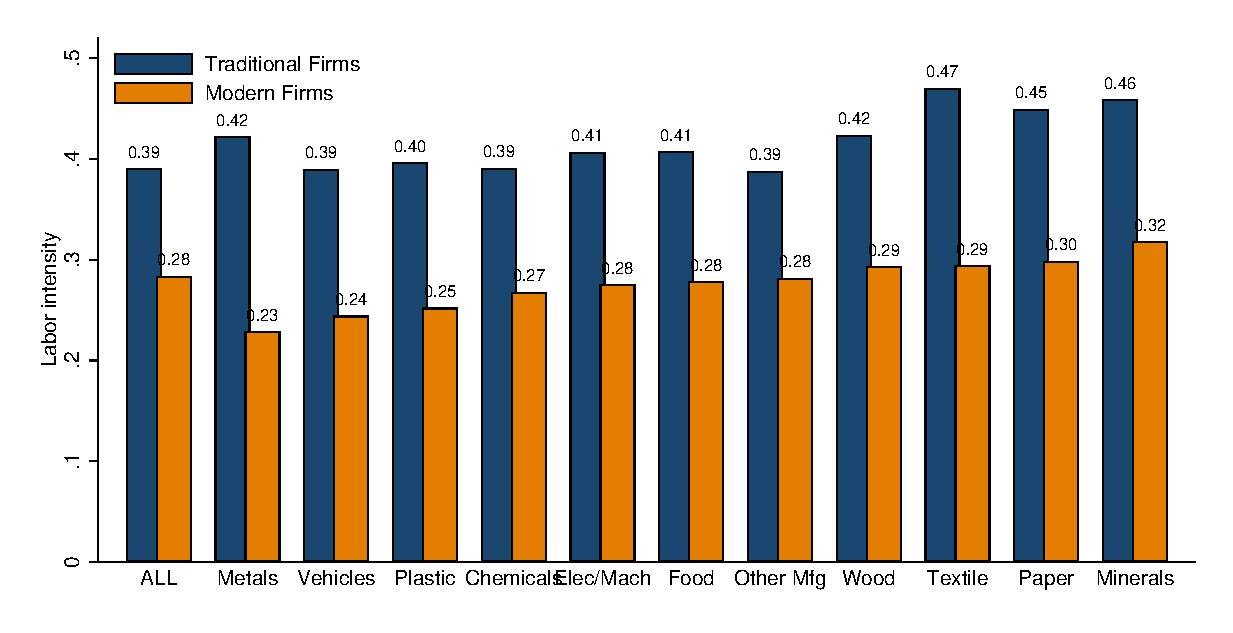
\includegraphics[scale=0.65]{fig/pattern_labor_intensity}
\par\end{centering}
\textbf{\footnotesize{}Notes}{\footnotesize{}: This figure shows our
estimates of output elasticity of labor by firm status in terms of
modern and traditional technology, for the manufacturing industry
as a whole, and by disaggregation, using firm-level data from WBES.
Section \ref{sec:Quantification_apdx} provides details about the
methodology that we apply to estimate production technologies and
assign firms into modern and traditional technological types.}{\footnotesize\par}
\end{figure}

\begin{figure}[H]
\caption{Labor Intensity according to Three Technology Types - Complementary
Pattern 1\label{fig:fact3_app}}

\begin{centering}
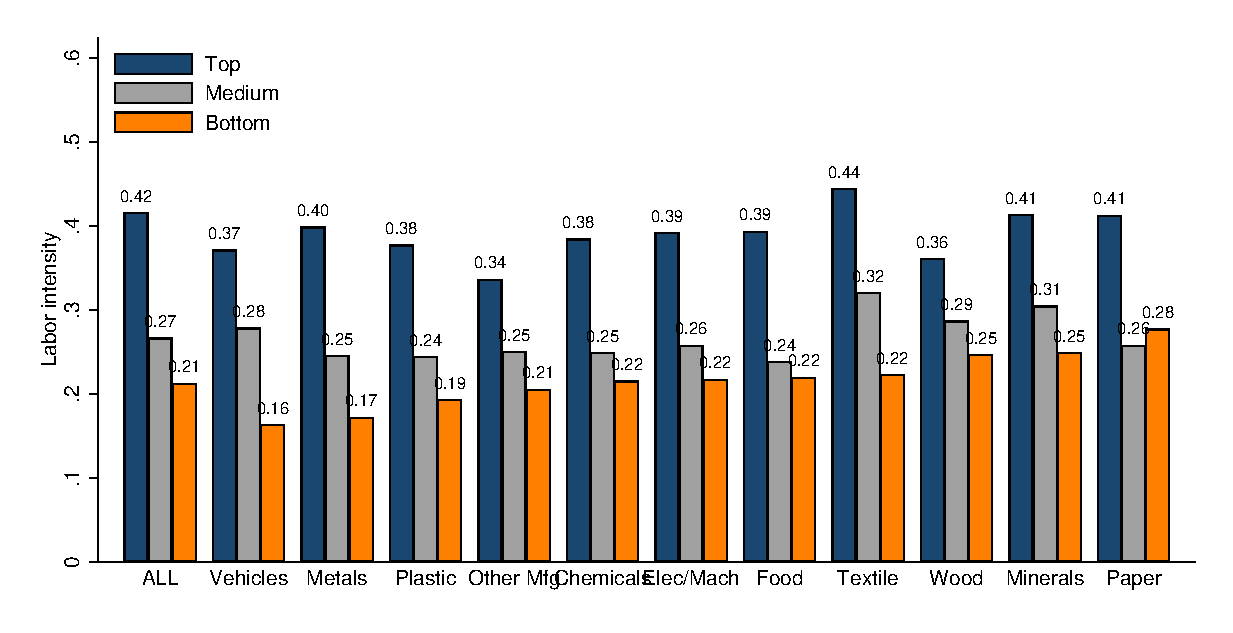
\includegraphics[scale=0.65]{fig/fact_3_labor_intensity_3_tech}
\par\end{centering}
\textbf{\footnotesize{}Notes}{\footnotesize{}: This figure replicates
the exercise in Figure \ref{fig:fact_share_labor_technology} but
using three technology regimes rather then two. Here, we split the
sample in terms of firm size according to three groups within each
sector of the economy: (1) those in the first quartile in the distribution
of firm size; (2) those in the bottom quartile in that distribution;
and (3) those in the second and third quartile.}{\footnotesize\par}
\end{figure}

\begin{figure}[H]
\caption{Welfare Cost of Misallocation in Closed Economies\label{fig:Welfare_Cost_Closed}}

\begin{centering}
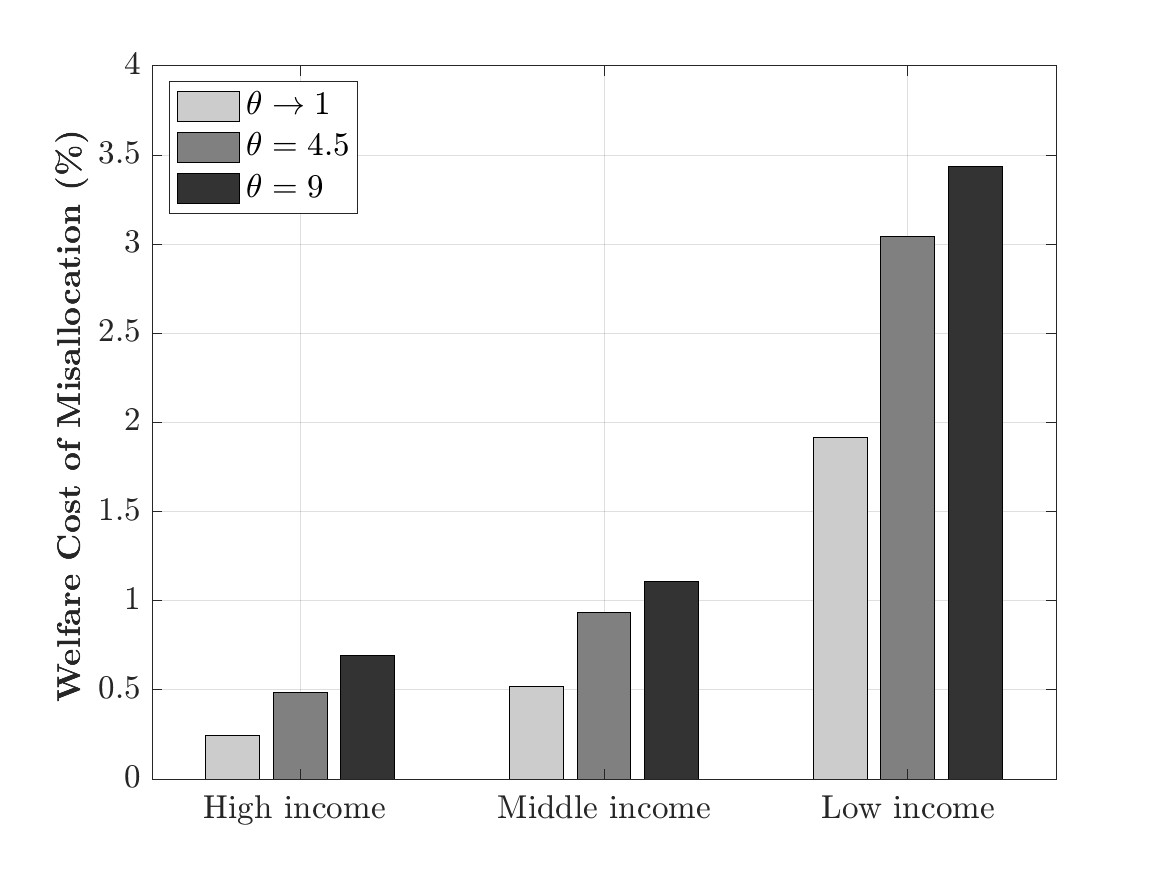
\includegraphics[scale=0.2]{fig/Distance_to_Frontier}
\par\end{centering}
\textbf{\footnotesize{}Notes}{\footnotesize{}: This figure shows the
distance to the efficient frontier (i.e., welfare costs of labor market
distortions) for closed economies. Quantifying the distance to the
efficient frontier of closed economies requires two counterfactuals.
First, we move economies to autarky by raising trade costs to infinity.
Second, in addition to moving economies to autarky, we eliminate their
labor market distortions. The difference between these two counterfactual
outcomes maps to the welfare cost of misallocation if countries were
operating as closed economies. Each bar shows our results by averaging
them across countries in the high, middle, and low-income groups,
evaluated at three different values of the technology elasticity ($\theta$).
The figure shows that the welfare cost of misallocation is larger
in low-income countries, and particularly more so when the technology
elasticity ($\theta$) is larger.}{\footnotesize\par}
\end{figure}

\begin{figure}[H]
\caption{Impact of Trade on Real Wage \emph{with} and \emph{without} Distortions\label{fig:Real-Wages-Main CF-apdx}}

\begin{centering}
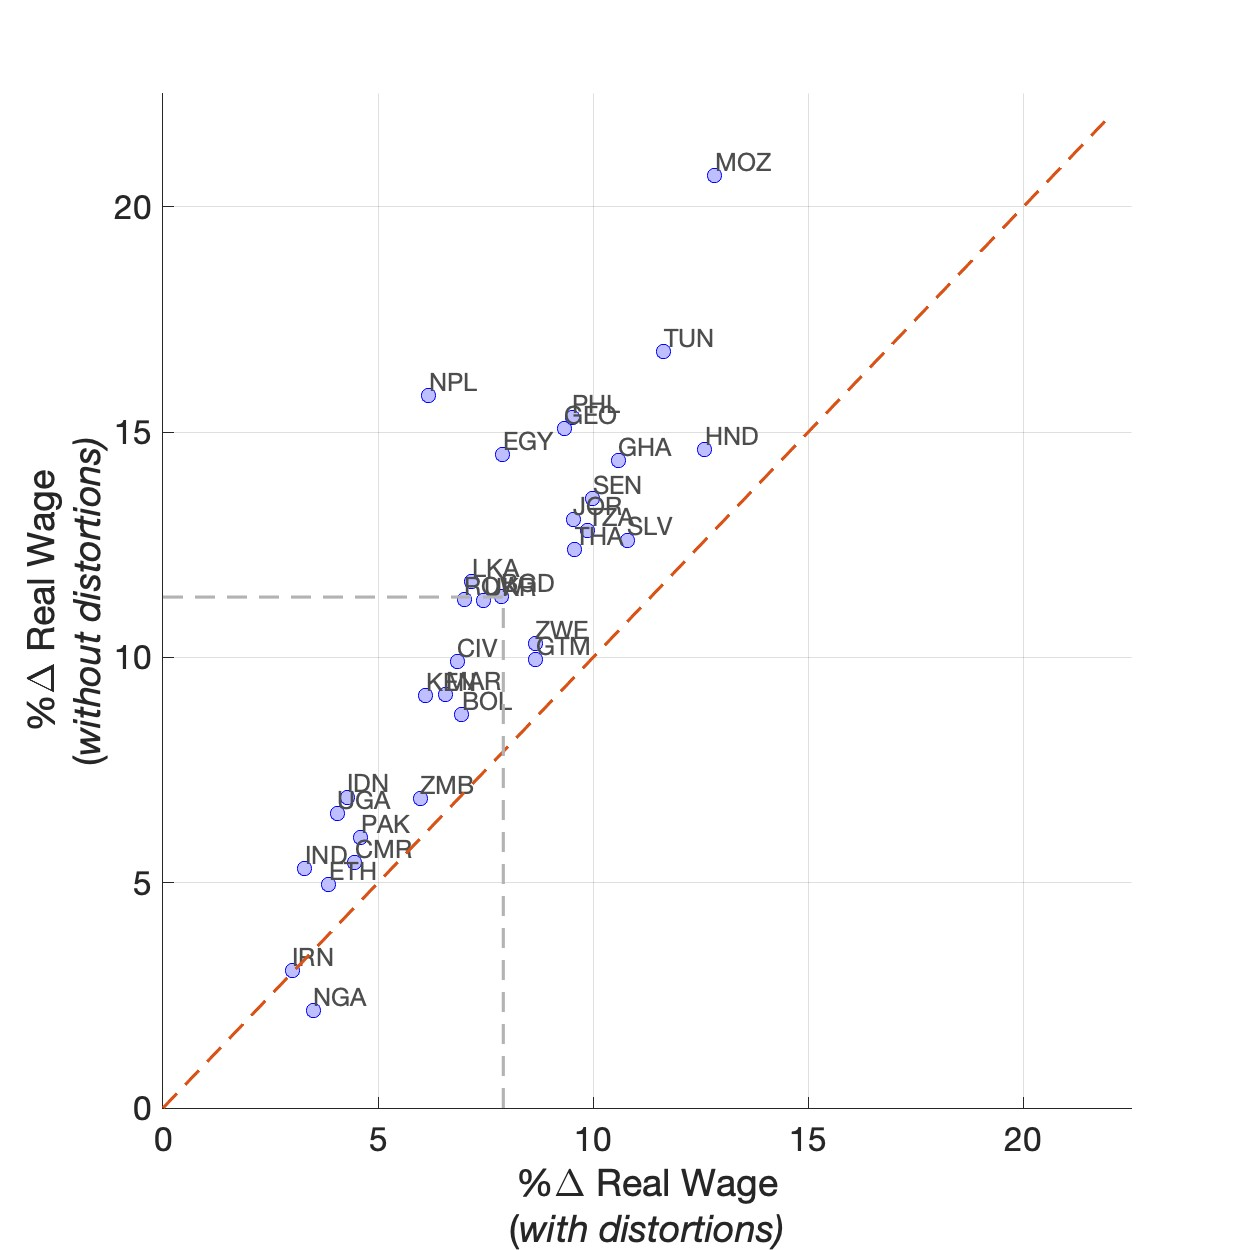
\includegraphics[scale=0.2]{fig/GFT_L}
\par\end{centering}
\textbf{\footnotesize{}Notes}{\footnotesize{}: This figure shows the
percentage change to real wage among low-income countries in response
to a 20\% reduction in trade costs. The x-axis reports changes under
the status quo labor wedges, the y-axis reports changes under no labor
wedges.}{\footnotesize\par}
\end{figure}

\begin{figure}[H]
\caption{Impact of Trade on Value Added per Worker in Manufacturing \emph{with}
and \emph{without} Distortions\label{fig:VA per worker Mfg-Main CF-apdx}}

\begin{centering}
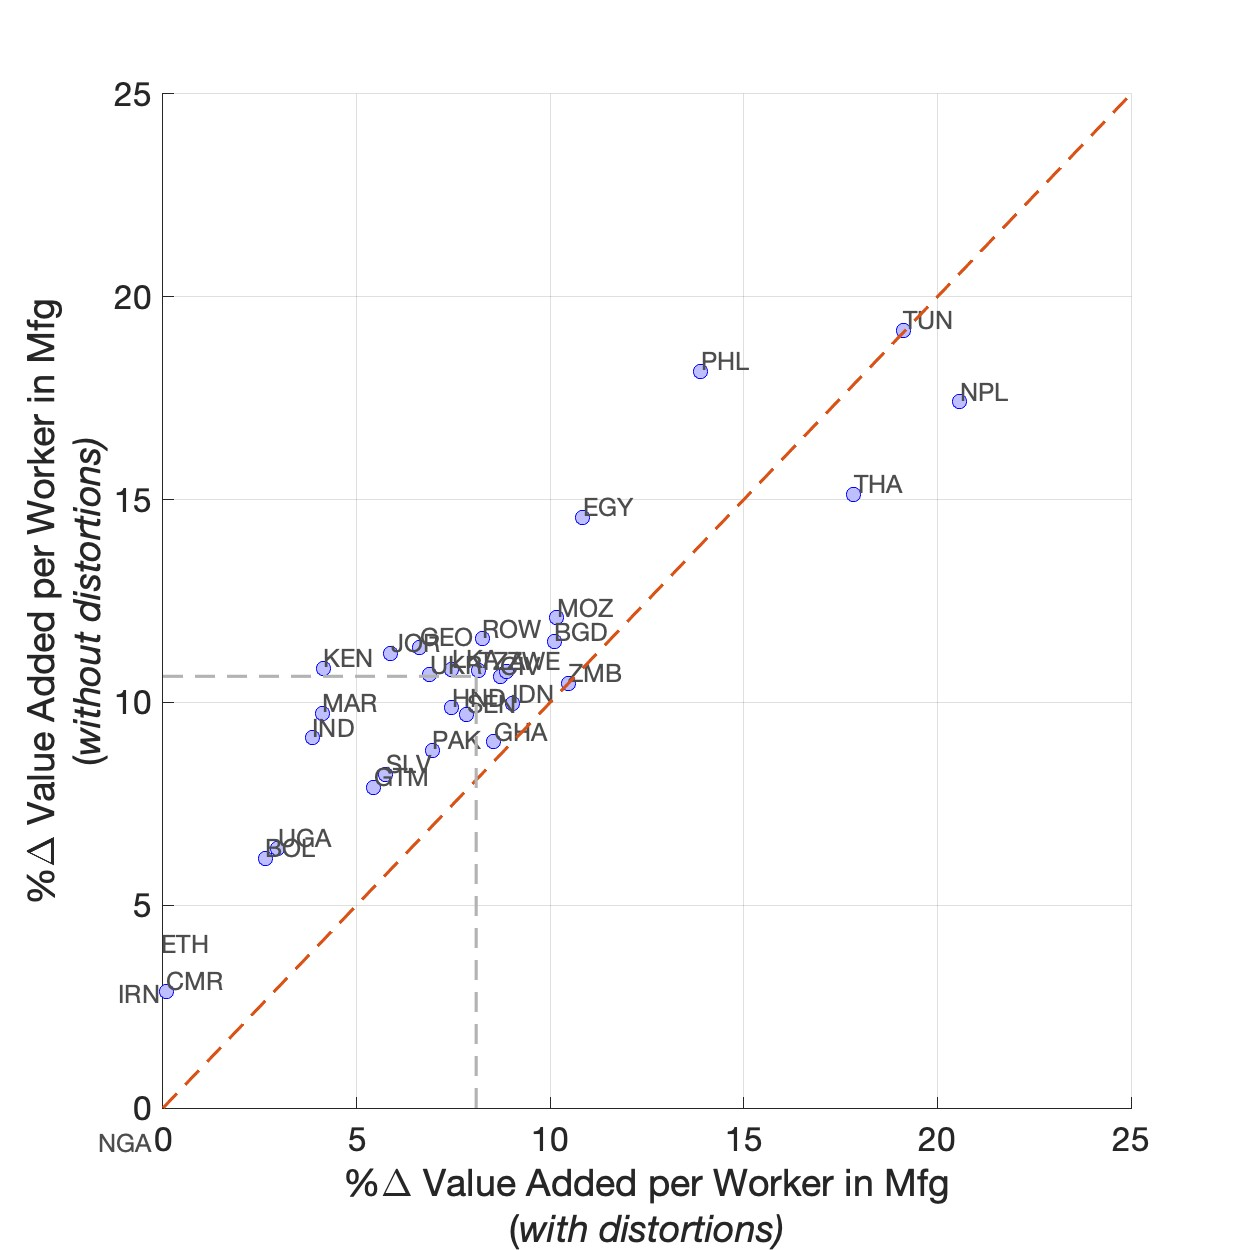
\includegraphics[scale=0.2]{fig/DiD_VAPW_mfg}
\par\end{centering}
\textbf{\footnotesize{}Notes}{\footnotesize{}: This figure shows the
percentage change to value added per worker in manufacturing among
low-income countries in response to a 20\% reduction in trade costs.
The x-axis reports changes under the status quo labor wedges, the
y-axis reports changes under no labor wedges.}{\footnotesize\par}
\end{figure}

\begin{figure}[H]
\caption{Impact of Trade on Welfare \emph{with} and \emph{without} Distortions\label{fig:Welfare-Main CF-apdx}}

\begin{centering}
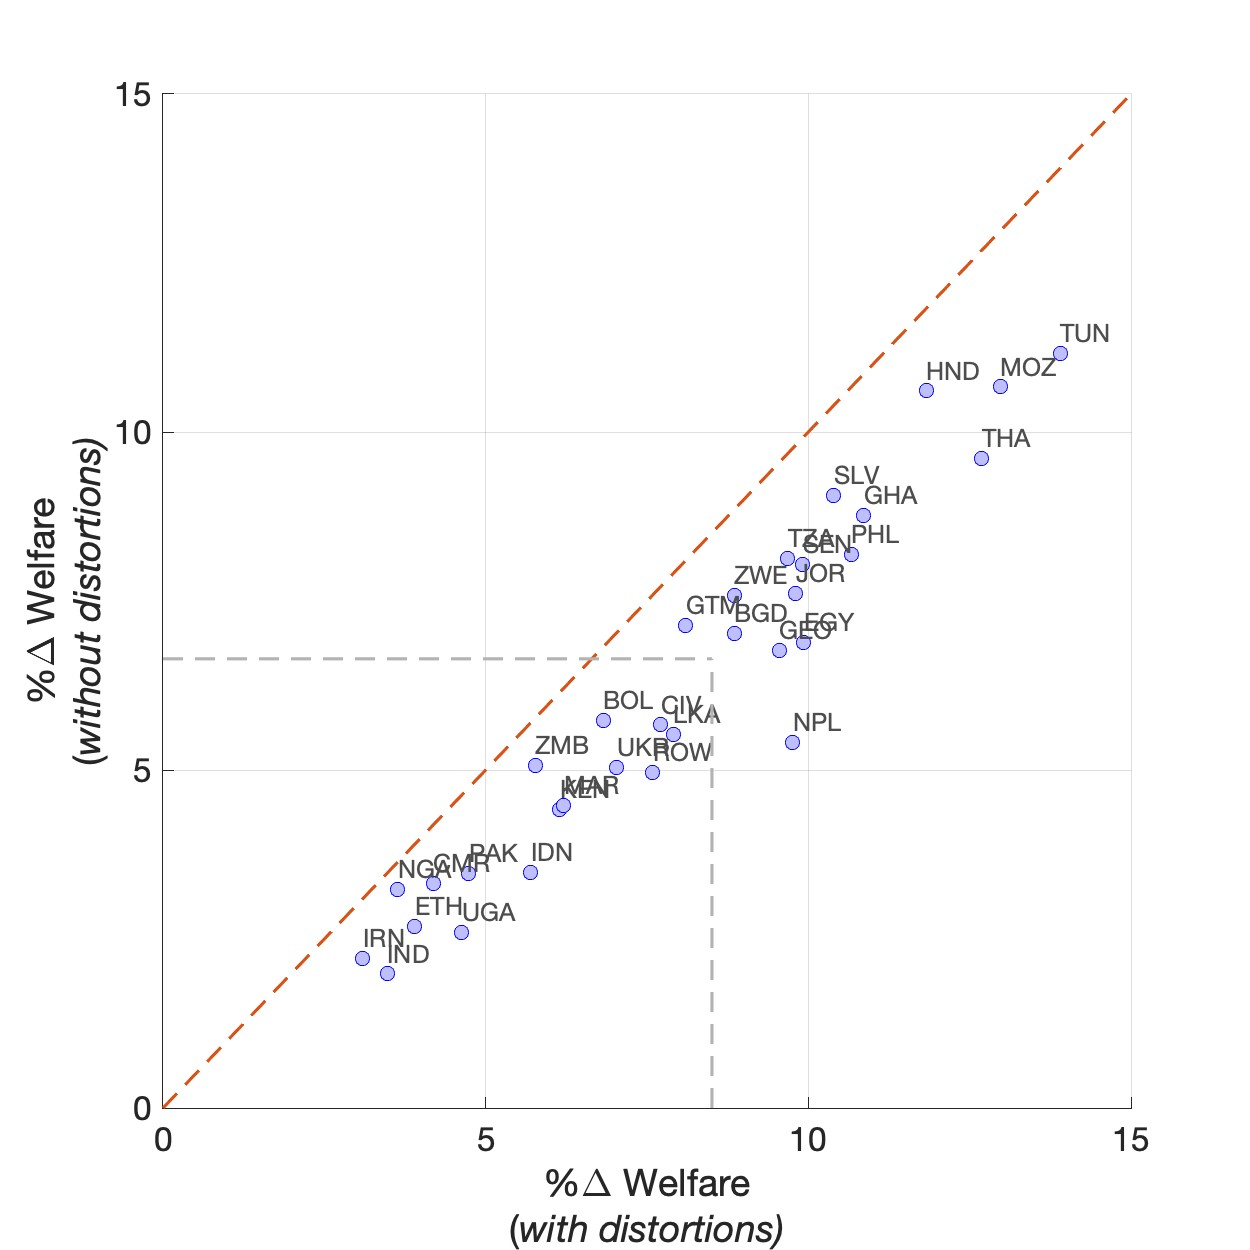
\includegraphics[scale=0.2]{fig/GFT_all}
\par\end{centering}
\textbf{\footnotesize{}Notes}{\footnotesize{}: This figure shows the
percentage change to aggregate welfare among low-income countries
in response to a 20\% reduction in trade costs. The x-axis reports
changes under the status quo labor wedges, the y-axis reports changes
under no labor wedges.}{\footnotesize\par}
\end{figure}

\begin{figure}[H]
\caption{\label{fig: trade vs APL (appendix)}Impact of Trade liberalization
on Aggregate labor Productivity across Low, Middle, and High-income
Countries}

\begin{centering}
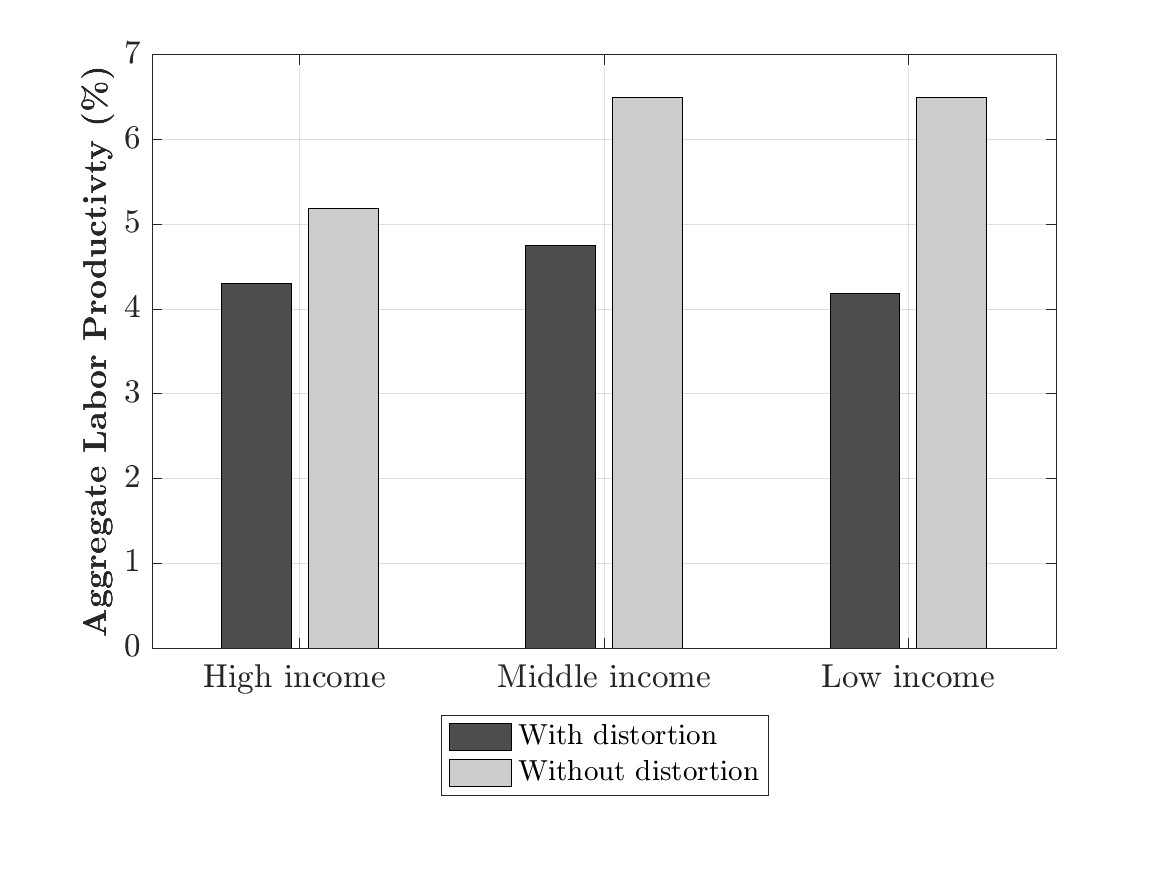
\includegraphics[scale=0.25]{fig/ALP_lomdhi}
\par\end{centering}
\textbf{\footnotesize{}Notes}{\footnotesize{}: This figure shows the
percentage change to aggregate labor productivity in response to a
20\% reduction in trade costs, averaging the results for low, middle,
and high-income country groups.}{\footnotesize\par}
\end{figure}

\begin{sidewaysfigure}[H]
\caption{Production Technology and Labor Wedges - Alternative Estimation Procedures\label{fig:apx_alternative_procedures}}

\begin{centering}
{\footnotesize{}}%
\begin{tabular}{ccrr}
\multicolumn{2}{c}{{\footnotesize{}\uline{Baseline}}} & \multicolumn{2}{c}{{\footnotesize{}\uline{Formal vs. Informal}}}\tabularnewline
{\footnotesize{}}\subfloat[Labor Intensity]{{\footnotesize{}}{\footnotesize\par}
\centering{}{\footnotesize{}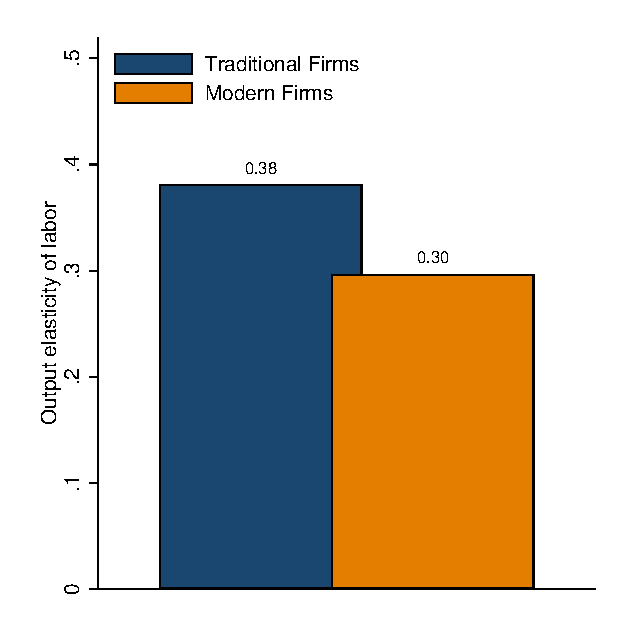
\includegraphics[scale=0.4]{fig/pattern_labor_intensity_modern}}{\footnotesize\par}} & {\footnotesize{}}\subfloat[Labor Wedges]{{\footnotesize{}}{\footnotesize\par}
\centering{}{\footnotesize{}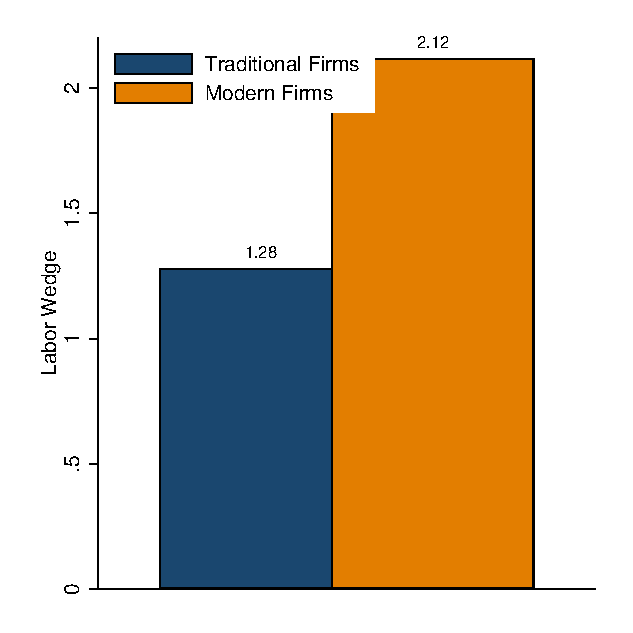
\includegraphics[scale=0.4]{fig/pattern_wedge_modern}}{\footnotesize\par}} & {\footnotesize{}}\subfloat[Labor Intensity]{{\footnotesize{}}{\footnotesize\par}
\centering{}{\footnotesize{}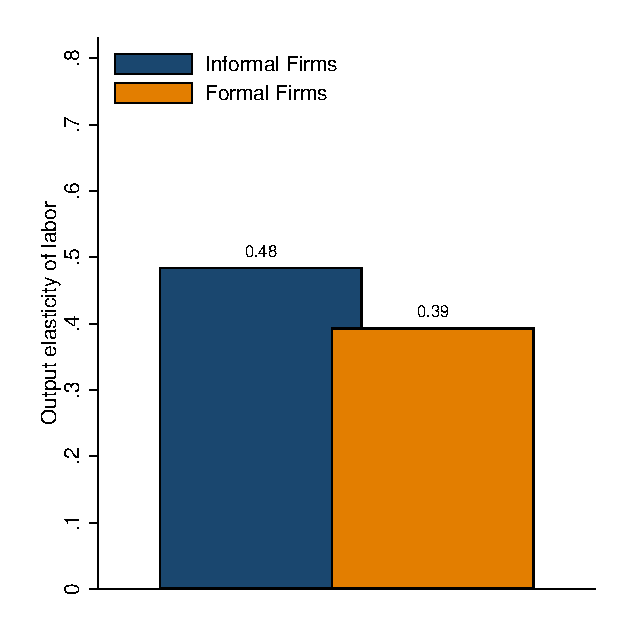
\includegraphics[scale=0.4]{fig/pattern_labor_intensity_formal}}{\footnotesize\par}} & {\footnotesize{}}\subfloat[Labor Wedges]{{\footnotesize{}}{\footnotesize\par}
\centering{}{\footnotesize{}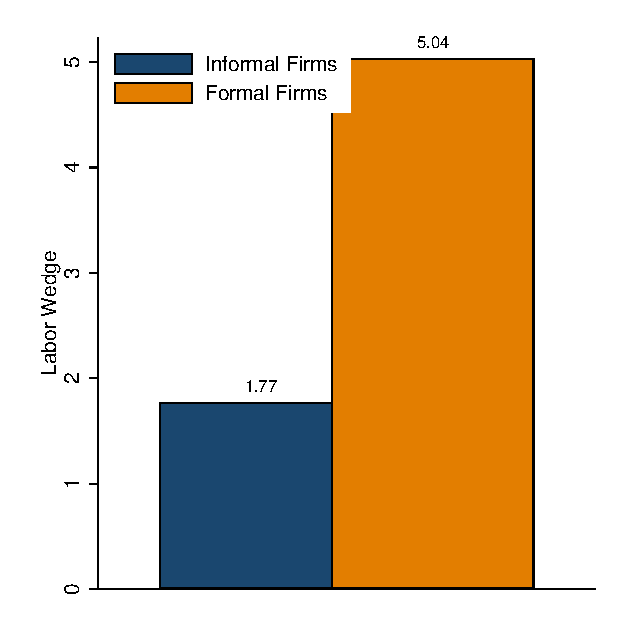
\includegraphics[scale=0.4]{fig/pattern_wedge_formal}}{\footnotesize\par}}\tabularnewline
\multicolumn{2}{c}{{\footnotesize{}\uline{Low Income}}} & \multicolumn{2}{c}{{\footnotesize{}\uline{High- and Middle-Income}}}\tabularnewline
{\footnotesize{}}\subfloat[Labor Intensity]{{\footnotesize{}}{\footnotesize\par}
\centering{}{\footnotesize{}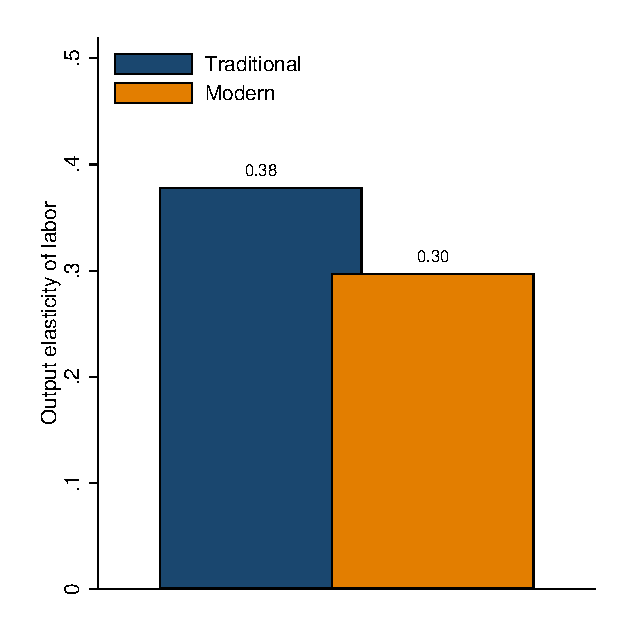
\includegraphics[scale=0.4]{fig/pattern_labor_intensity_multiple_low_income}}{\footnotesize\par}} & {\footnotesize{}}\subfloat[Labor Wedges]{{\footnotesize{}}{\footnotesize\par}
\centering{}{\footnotesize{}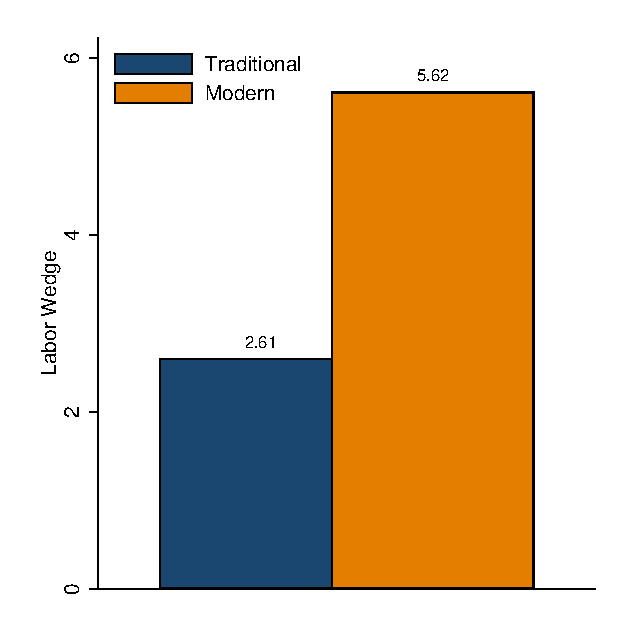
\includegraphics[scale=0.4]{fig/pattern_wedge_multiple_low_income}}{\footnotesize\par}} & {\footnotesize{}}\subfloat[Labor Intensity]{{\footnotesize{}}{\footnotesize\par}
\centering{}{\footnotesize{}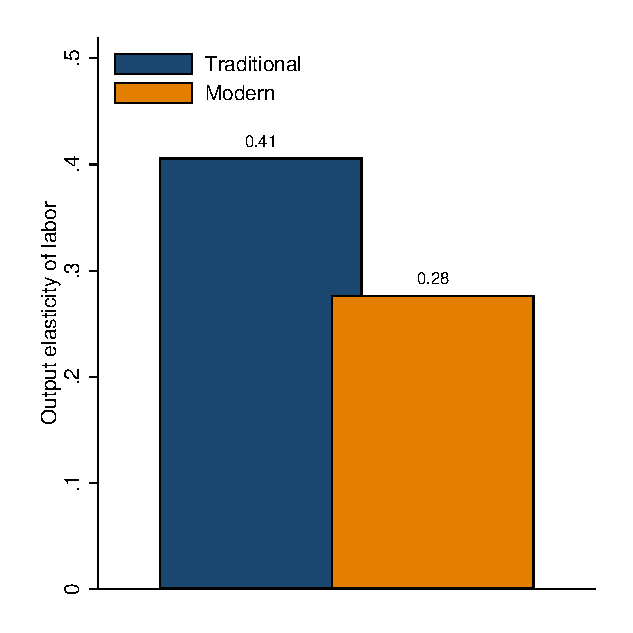
\includegraphics[scale=0.4]{fig/pattern_labor_intensity_multiple_high_income}}{\footnotesize\par}} & {\footnotesize{}}\subfloat[Labor Wedges]{{\footnotesize{}}{\footnotesize\par}
\centering{}{\footnotesize{}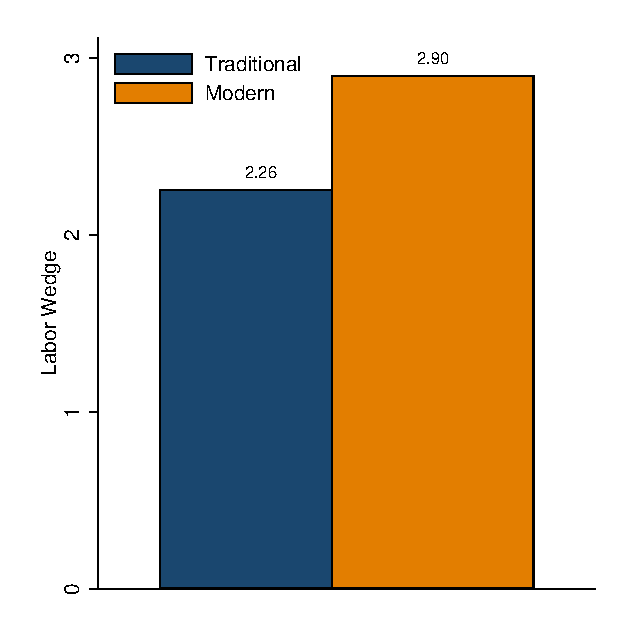
\includegraphics[scale=0.4]{fig/pattern_wedge_multiple_high_income}}{\footnotesize\par}}\tabularnewline
\end{tabular}{\footnotesize\par}
\par\end{centering}
\textbf{\footnotesize{}Notes}{\footnotesize{}: These figures show
estimates of the labor intensity and the labor wedges discussed in
Section \ref{subsec:Robustness}. Panels (a) and (b) report the labor
intensity and labor wedge for our baseline analysis. Panels (c) and
(d) the labor intensity and labor wedges when we classify firms into
modern and traditional based on whether they are formal or informal,
as discussed in Section \ref{subsec:formal_vs_informal}. Panels (e)
to (h) report our results when we separately estimate the labor intensities
and wedges based on whether the country is low-income or middle- and
high-income, as discussed in Section \ref{subsec:heterogeneous_labor_intensities}.}{\footnotesize\par}
\end{sidewaysfigure}

\begin{sidewaysfigure}[H]
\caption{Robustness Check on Trade Liberalization \label{fig:robustness_trade_liberalization_apdx}}

\begin{centering}
{\footnotesize{}}%
\begin{tabular}{ccrr}
\multicolumn{2}{c}{{\footnotesize{}\uline{Multiple Technologies}}} & \multicolumn{2}{c}{{\footnotesize{}\uline{Formal vs. Informal}}}\tabularnewline
\subfloat[ALP]{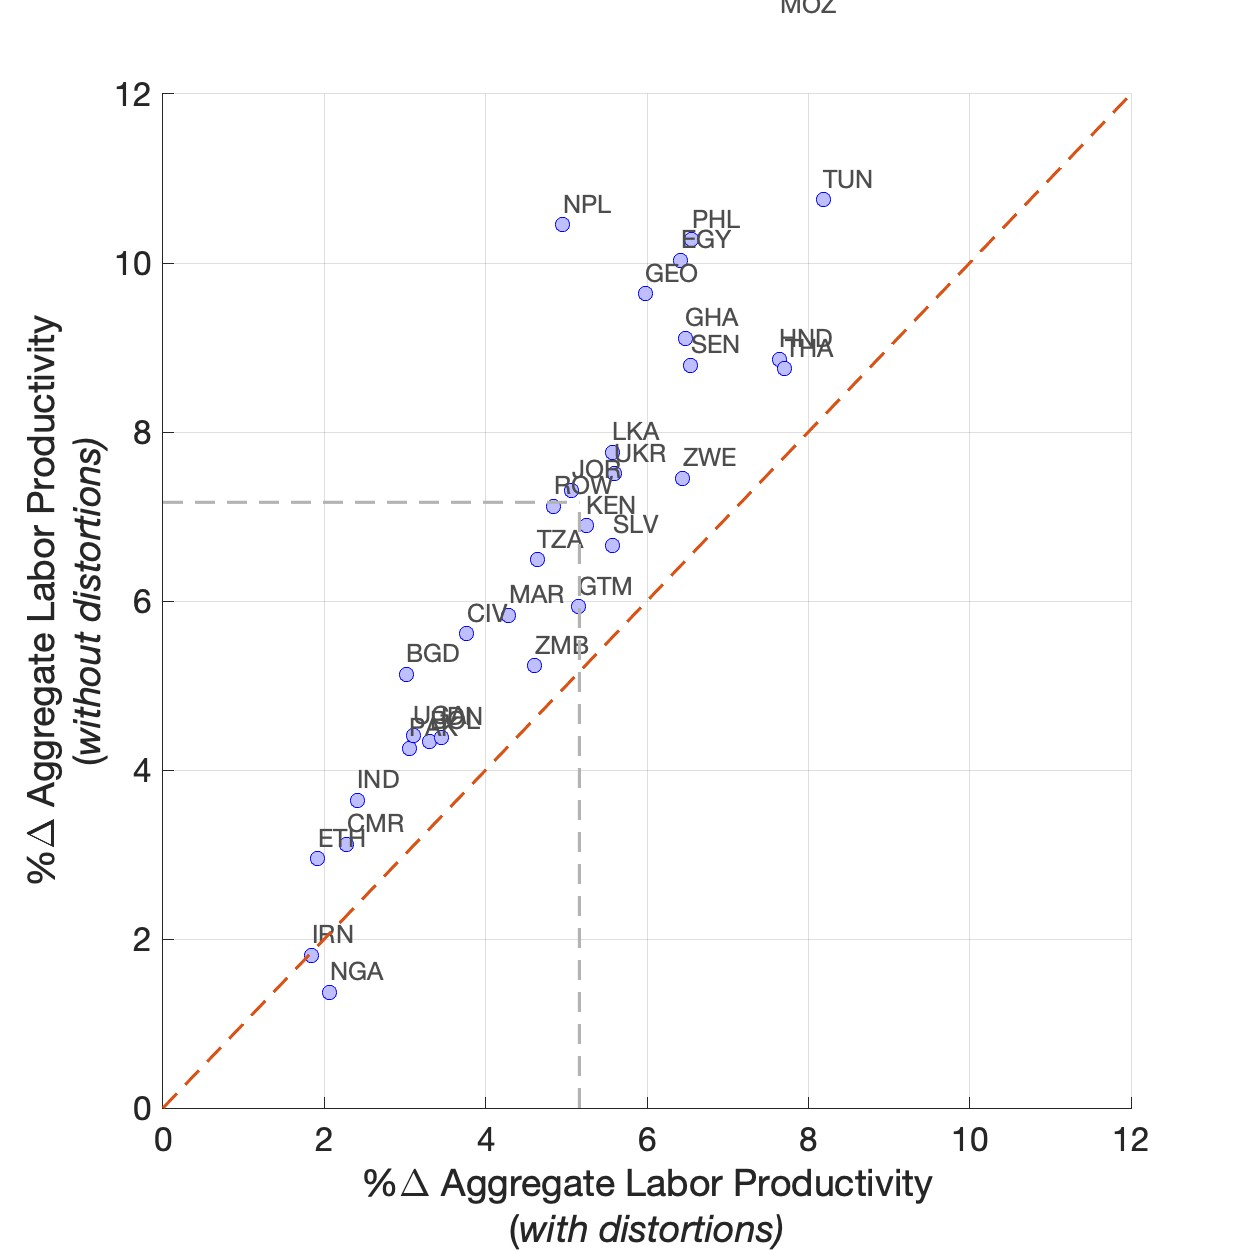
\includegraphics[scale=0.13]{fig/ALP_multiple}} & \subfloat[Real Wage]{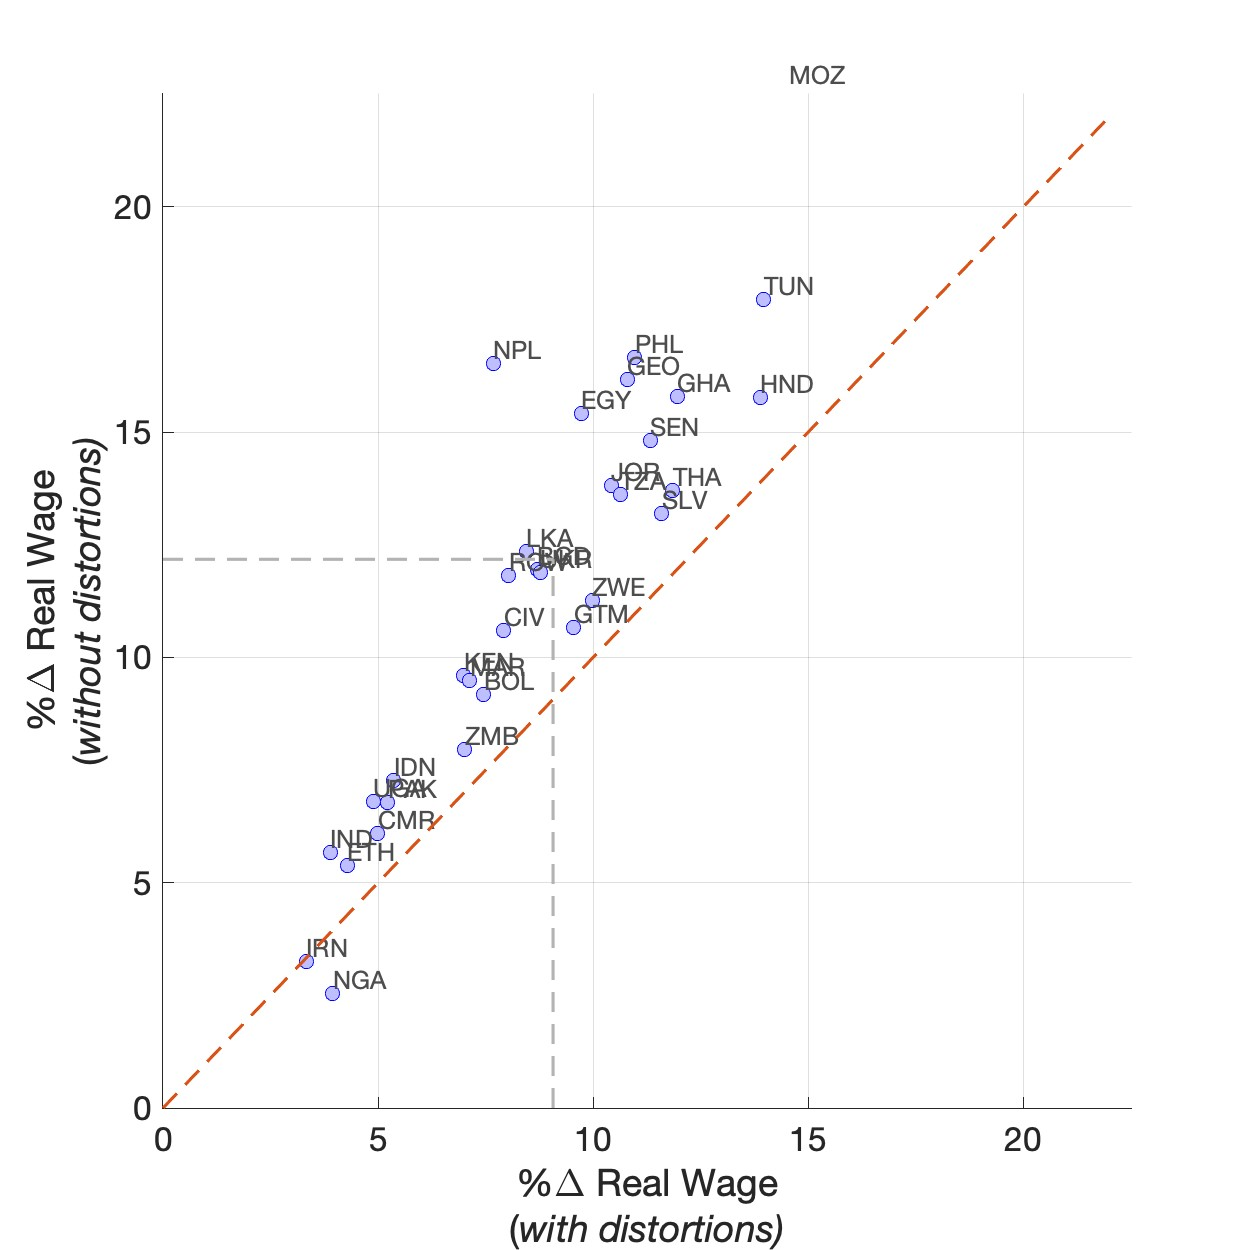
\includegraphics[scale=0.13]{fig/GFT_L_multiple}} & \subfloat[ALP]{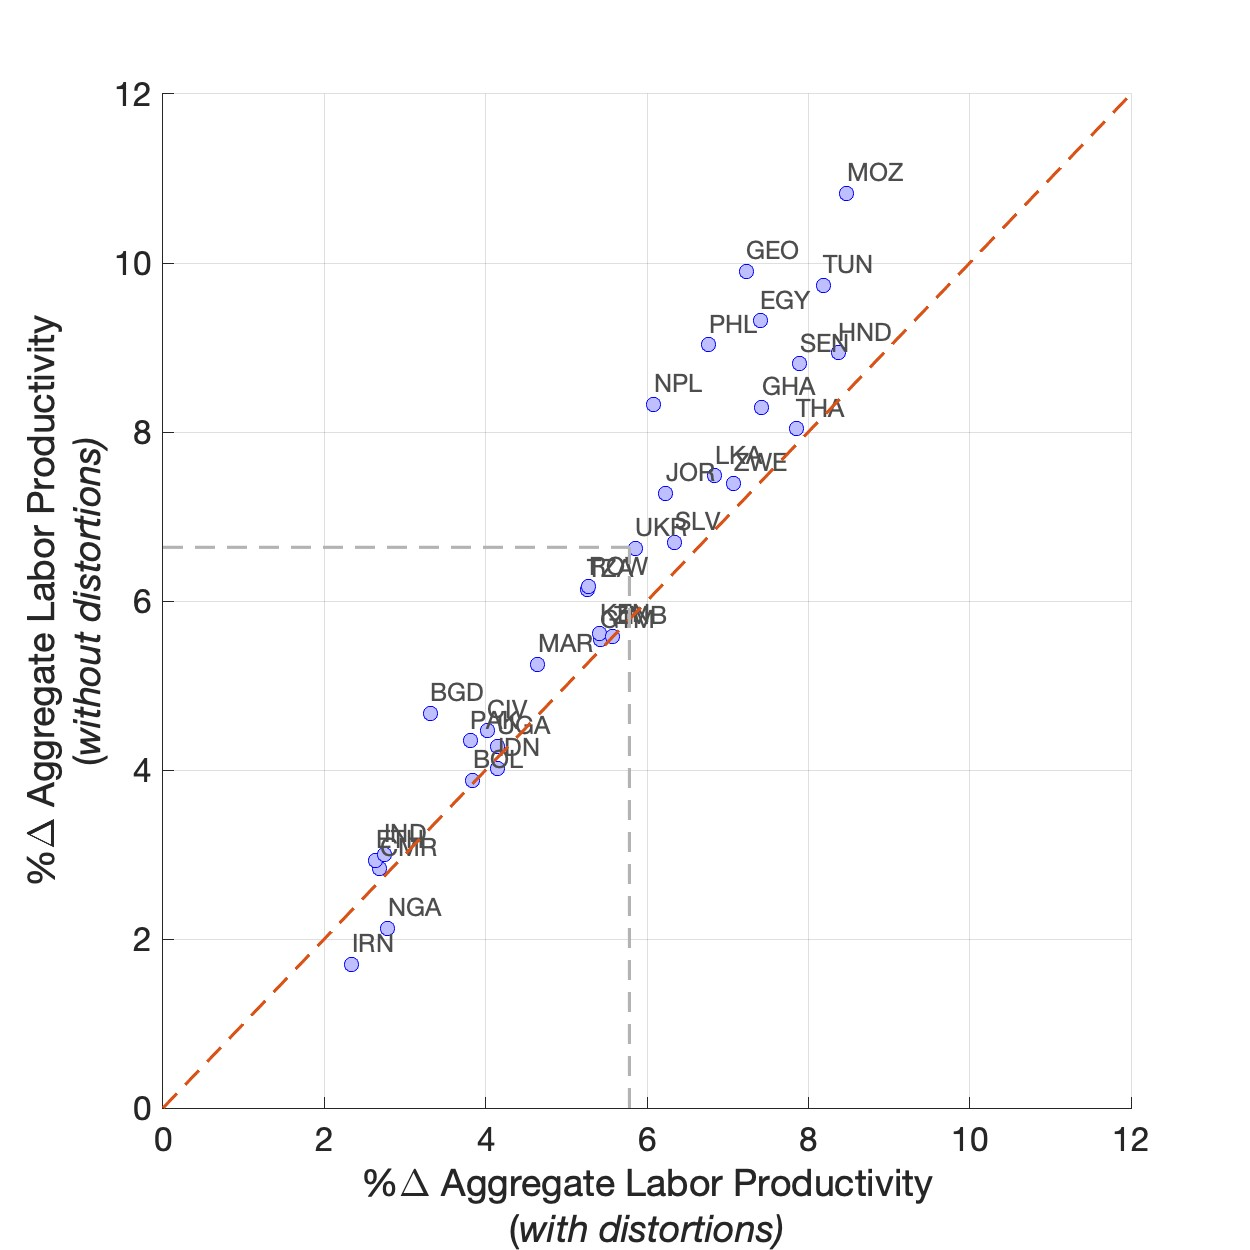
\includegraphics[scale=0.13]{fig/ALP_formal}} & \subfloat[Real Wage]{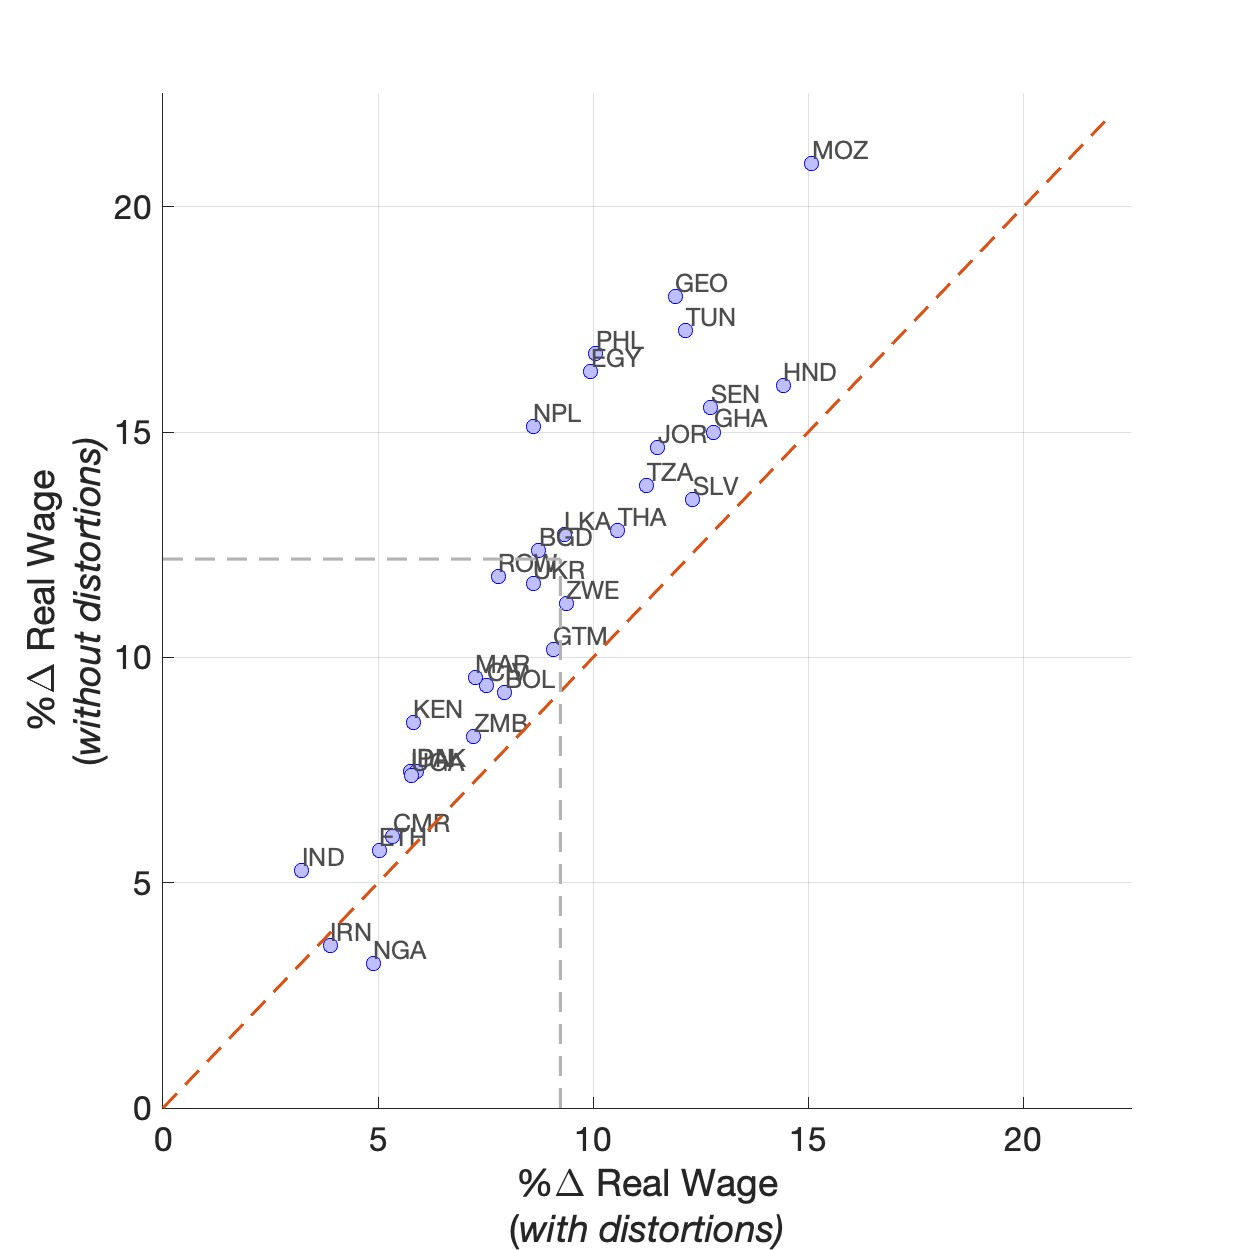
\includegraphics[scale=0.13]{fig/GFT_L_formal}}\tabularnewline
\multicolumn{2}{c}{{\footnotesize{}\uline{Low Theta}}} & \multicolumn{2}{c}{{\footnotesize{}\uline{High-Theta}}}\tabularnewline
\subfloat[ALP]{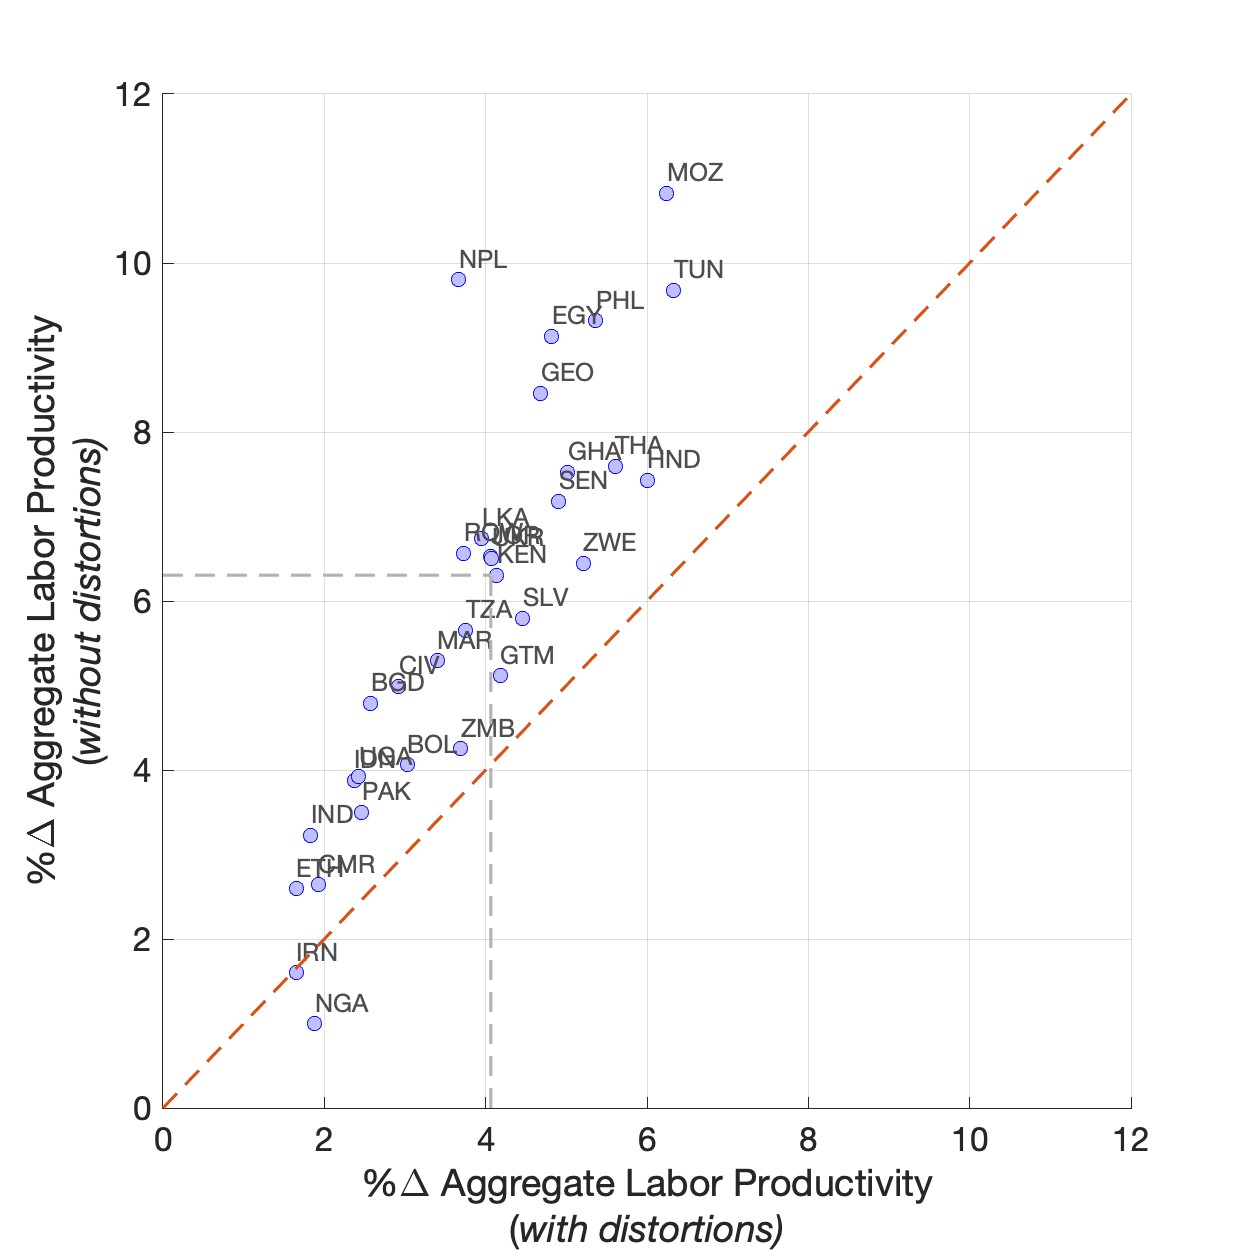
\includegraphics[scale=0.13]{fig/ALP_LowTheta}} & \subfloat[Real Wage]{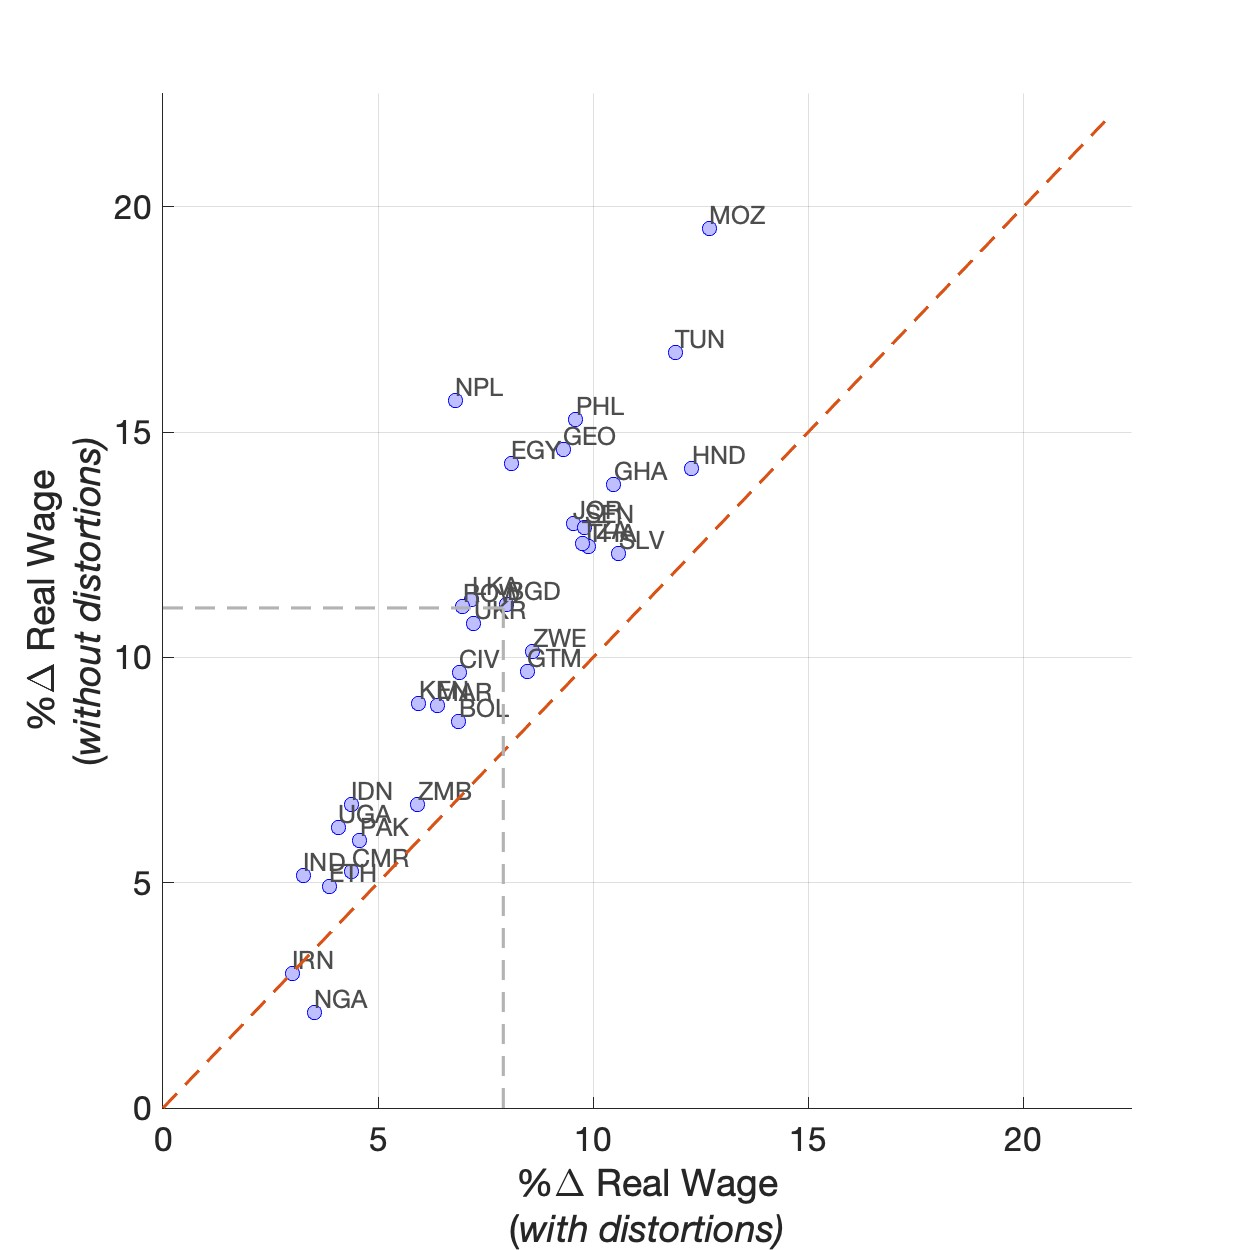
\includegraphics[scale=0.13]{fig/GFT_L_LowTheta}} & \subfloat[ALP]{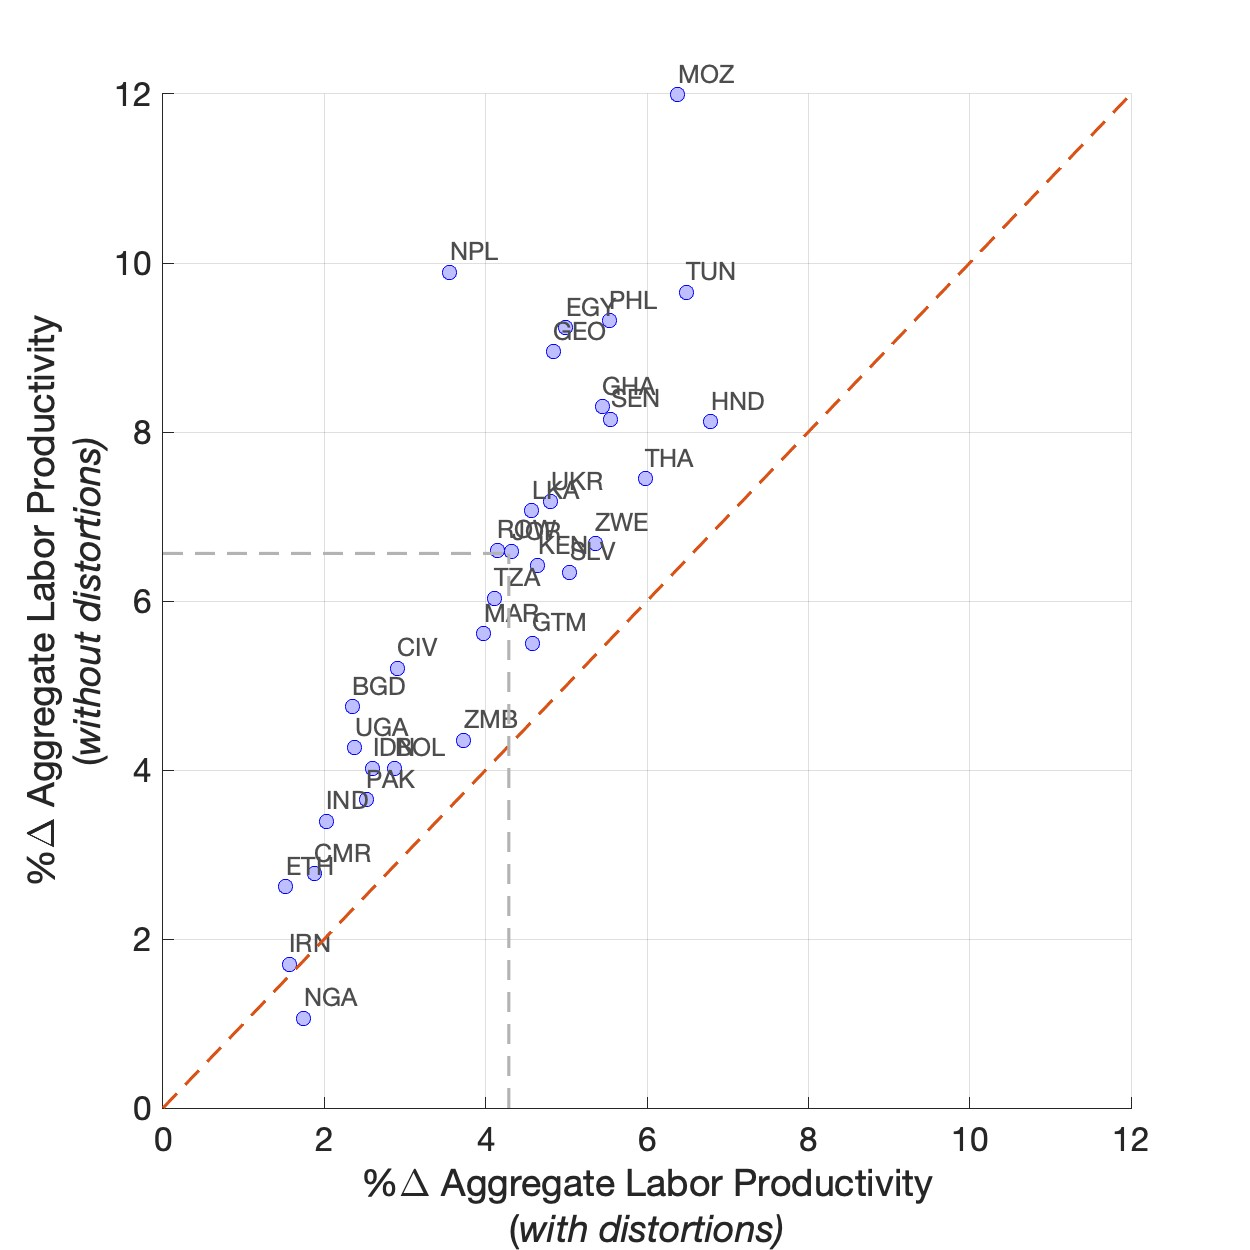
\includegraphics[scale=0.13]{fig/ALP_HighTheta}} & \subfloat[Real Wage]{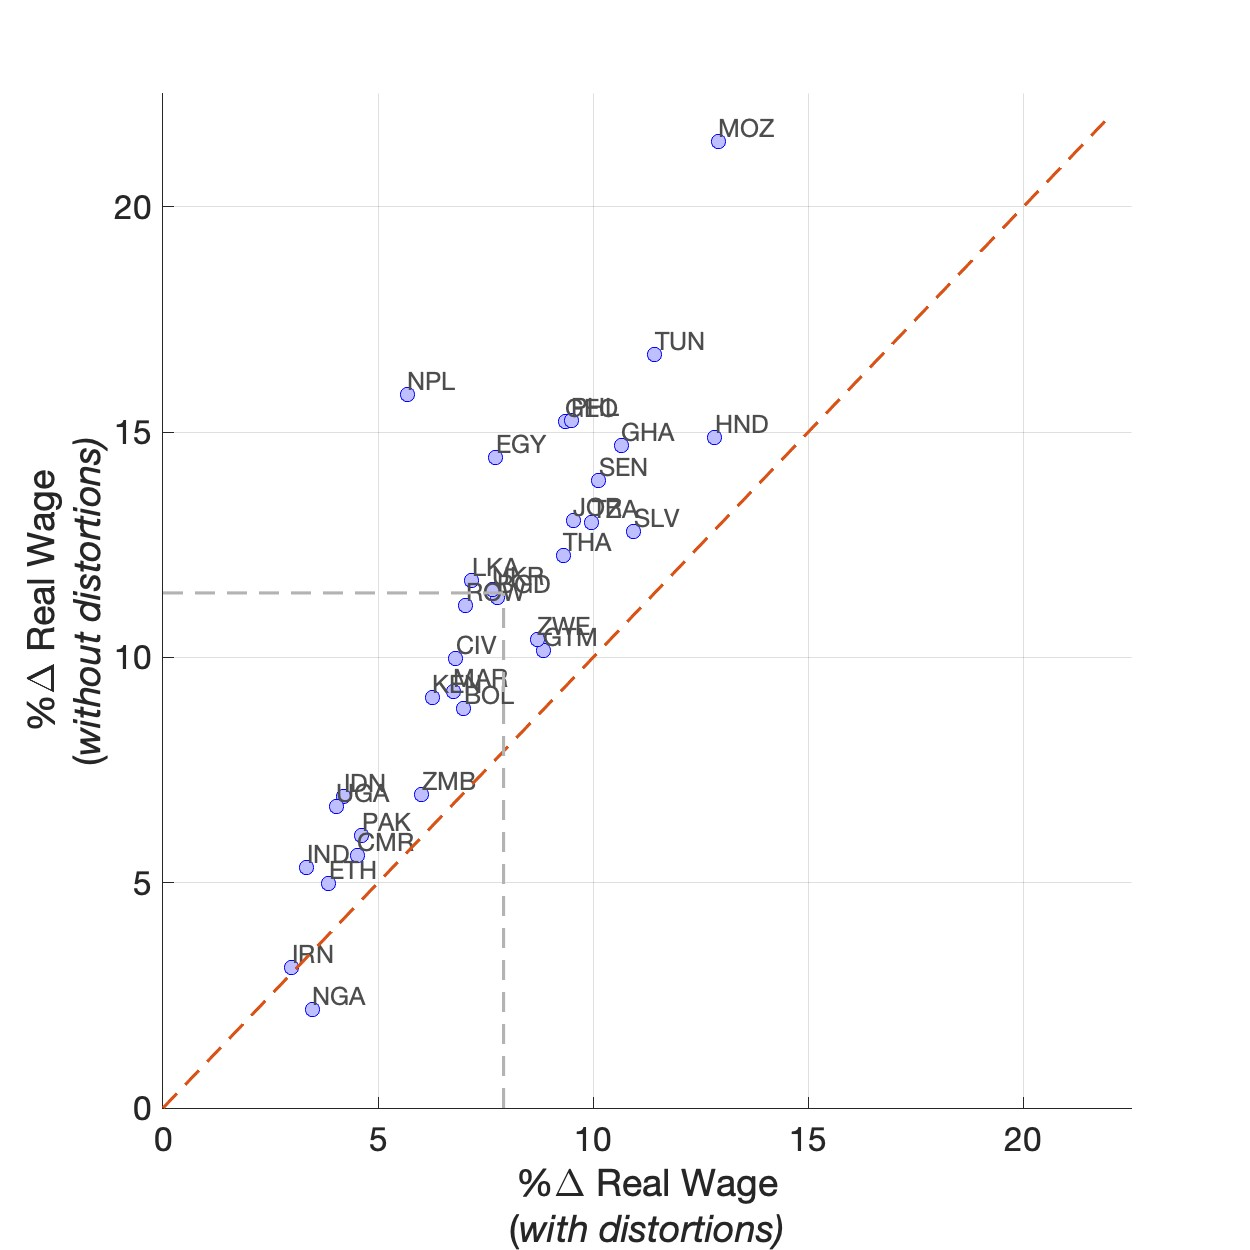
\includegraphics[scale=0.13]{fig/GFT_L_HighTheta}}\tabularnewline
\end{tabular}{\footnotesize\par}
\par\end{centering}
\textbf{\footnotesize{}Notes}{\footnotesize{}: These figures show,
for each calibration procedure, the percentage change to aggregate
labor productivity and real wage in response to a 20\% reduction in
trade costs. Results are discussed in Section \ref{subsec:Robustness}.}{\footnotesize\par}
\end{sidewaysfigure}

\begin{figure}[H]
\caption{\label{fig: robustness - theta (appendix)}Impact of Trade liberalization
on Aggregate Labor Productivity and Technology Adoption along Different
Values of the Technology Elasticity}

\begin{centering}
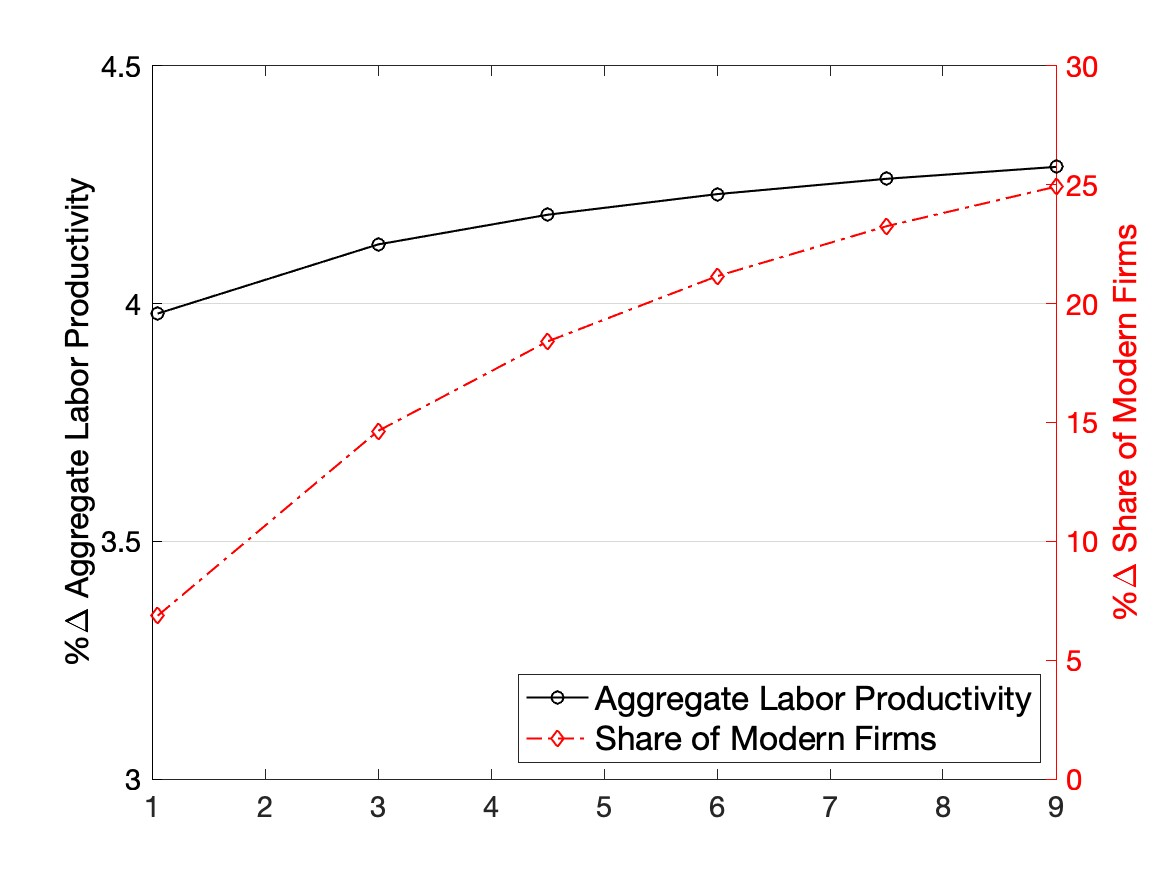
\includegraphics[scale=0.25]{fig/Results_Theta_ALP_x}
\par\end{centering}
\textbf{\footnotesize{}Notes}{\footnotesize{}: This figure shows,
for each value of the technology elasticity ($\theta$) on the x-axis,
the percentage change (averaged across low income countries) to the
share of modern firms (right-hand side y-axis) and aggregate labor
productivity (left-hand side y-axis) in response to a 20\% reduction
in trade costs.}{\footnotesize\par}
\end{figure}

%\newpage{}

%\section*{Appendix References}

%\bibliographystyle{apalike}
%\bibliography{biblio}

%\begin{btSect}[econometrica]{bibliography}
%\btPrintCited
%\end{btSect}
%\end{btUnit}

\end{document}
